\documentclass[11pt,a4paper,titlepage,spanish]{article}
\usepackage[left=1.5cm,top=2.5cm,right=1.5cm,bottom=2.5cm]{geometry} 
\usepackage[utf8]{inputenc}
\usepackage[spanish, es-tabla]{babel} %esto es para que aparezca "tabla" en lugar de "cuadro" al poner título a una tabla
\usepackage[T1]{fontenc}


%\usepackage{bbm}
\usepackage{amsthm,amsmath,mathrsfs}
\usepackage{hyperref}
\usepackage{color}
\usepackage{subfig}
\usepackage{float}

\usepackage[pdftex]{graphicx}
\DeclareGraphicsExtensions{.pdf,.png,.jpg,.bmp}

\newcommand{\HRule}{\rule{\linewidth}{0.5mm}}

% --- Para el encabezado
%\usepackage{fancyhdr}
%\fancyhead[L]{Preguntas teoricas} \fancyfoot[C]{\thepage}
%\pagestyle{fancy}
% -------------------------------------------------------- %
%opening
\title{Proyecto de grado\\ ``Análisis de video en Biomecánica''}
\author{Gonzalo Pereira. Mauricio Ramos, Guillermo Ottado, Andréi Guchin.}
\date {}

\begin{document}

\maketitle

\newpage
\tableofcontents
%\printindex
\newpage

%\begin{abstract}
%\begin{center}
%Documentación
%\end{center}
%\end{abstract}

%\clearpage


%%%%%%%%%%%%%%%%%%%%%%%%%%%%%%%%%%%%%%%%%%%%%%%%%%%%%%%%%%%%%%%%%%%%%%%%%%%%%%
%%%%%%%%%%%%%%%%%%%%%%%%%%%%%%%%%%%%%%%%%%%%%%%%%%%%%%%%%%%%%%%%%%%%%%%%%%%%%%
\chapter{Introducción}
%%%%%%%%%%%%%%%%%%%%%%%%%%%%%%%%55%%%%%%%%%%%%%%%%%%%%%%%%%%%%%%%%%%%%%%%%%%%%%%%%%%%%%%%%%%%%%%%%%%%%%%%%%%%%%%%%%%%%%%%%%%%%%%%%%
% requerimientos,Hacer como una sinopsis.
%%%%%%%%%%%%%%%%%%%%%%%%%%%%%%%%%%%%%%%%%%%%%%%%%%%%%%%%%%%%%%%%%%%%%%%%%%%%%%%%%%%%%%%%%%%%%%%%%%%%%%%%%%%%%%%%%%%%%%%%%%%%%%%%%%%

Este documento presenta las tareas realizadas en el marco del proyecto de fin de carrera ``Análisis de Video en Biomecánica'' realizado en la Facultad de Ingeniería, Universidad de la República (UdelaR). A continuación, se hace una introducción a la problemática encontrada, en función de la cual se plantea el objetivo del proyecto y una breve descripción de las soluciones actualmente disponibles.
\vspace{5 mm}

Especialistas de distintos ámbitos académicos o profesionales se encuentran habitualmente en la necesidad de realizar estudios del movimiento del cuerpo humano. Esta tarea implica registrar la posición de miembros o articulaciones en el espacio y su correspondiente evolución en el tiempo.
\\ 

Algunos ejemplos correspondientes a distintas áreas que ilustran estas necesidades son:

\begin{itemize}
\item A \emph{nivel asistencial}, en el área de \emph{fisioterapia}. Para realizar un seguimiento de la evolución de un paciente resulta importante en muchos casos conocer en detalle el movimiento, posición, etc. de la articulación o miembro afectado para llevar un control del mismo durante la rehabilitación y así poder determinar con mayor exactitud el estado y la evolución del paciente.
\item \emph{Investigación académica en biomecánica}. Diversos proyectos se llevan a cabo en las universidades sobre esta temática, por ejemplo, en la Facultad de Ingeniería de la Udelar  se realizó el estudio comparativo de la patada delfín y la patada “crawl” respecto al nado de los peces por ondulación, tratando de explicar cómo la misma puede ser propulsiva. Para ello se analizaron videos de nadadores olímpicos mediante los cuales se obtuvo una secuencia temporal de las posiciones de diferentes partes del cuerpo durante varios ciclos de patada\footnote{\textcolor{blue}{\scriptsize{\underline{\url{ http://www.fing.edu.uy/ingenieriademuestra2011/proyectos/proyectos-del-instituto-de-f\%C3\%ADsica}}}}. Accedido 20-12-14}.
\item \emph{Medidas de performance en el deporte de alto nivel}. Cuando se habla de entrenamiento deportivo se hace referencia tanto a la mejora del rendimiento del atleta como a la optimización de las capacidades en función del deporte en el que se desempeña. La técnica deportiva está relacionada directamente con la optimización de estas capacidades por lo que una buena técnica permite el mejor aprovechamiento de las posibilidades físicas del atleta garantizando mejores resultados. Las mejores soluciones para la optimización de la técnica de un deportista consisten en el análisis de videos donde se puede estudiar en detalle cada uno de los movimientos del  mismo.
\item \emph{Animación 3D}. Probablemente el más conocido de estos ejemplos, tanto en el diseño de videojuegos como en películas, programas de televisión o comerciales, muchas veces se requiere capturar el movimiento de un actor para interpretar un personaje ficticio y que sus movimientos parezcan lo más natural posible. En el medio local existen empresas que se dedican a esto, tales como Mopix \footnote{\textcolor{blue}{\underline{\url{http://mopix.com.uy/}}}. Accedido 20-12-14}.
\end{itemize}

En este contexto, el análisis de video  es  una  herramienta  fundamental para la recolección y estudio de datos. El seguimiento de puntos de referencia se utiliza para el cálculo de posición y otras variables asociadas como son la velocidad, la aceleración y por ende desplazamientos. Trabajar con video permite además estudiar secuencialmente situaciones estáticas en el tiempo. El seguimiento de dichos puntos resultaría tedioso si se hiciera manualmente por lo que resulta necesario contar con una herramienta que realice esta tarea automáticamente.
\\ 

A raíz de esto, se crean los \emph{sistemas de captura de movimiento}, que se definen como un conjunto de dispositivos y software que a partir de la grabación del movimiento de una persona (o cualquier otra cosa), es capaz de trasladar dicho movimiento a un modelo digital para diferentes fines.
\\ 

Los ejemplos mencionados anteriormente definen distintos casos de uso con características disímiles, de manera que la búsqueda de una solución única que abarque las necesidades particulares de todos ellos resulta compleja. Por ejemplo, en el ámbito deportivo la velocidad del movimiento es una variable importante a tener en cuenta para desarrollar una solución, de esta variable depende la elección tanto del sistema de adquisición como de los algoritmos más eficaces para el registro del movimiento.  De igual manera definir la portabilidad del sistema depende de si la actividad a relevar es en condiciones de laboratorio controladas o al aire libre, debido a la protección y transporte de equipos o las variaciones en las condiciones de iluminación, ruido, etc..
\\ 

Al  día  de  hoy, las  soluciones  de  software  disponibles que  podrían  asistir al especialista en su tarea, son mayormente comerciales. Las pocas alternativas de código abierto, carecen de las características necesarias para el especialista o están enfocadas hacia otras áreas de aplicación. Contar con este tipo de herramientas es fundamental para las necesidades de los equipos de profesionales, cuya alternativa son productos comerciales de alto costo.
\\ 

En virtud de estas necesidades, este proyecto busca \emph{relevar y caracterizar los distintos casos de uso para un sistema de captura de movimiento, seleccionar uno que sea representativo y suficientemente general para poder realizar una aplicación básica y funcional de código abierto de análisis de video, que proporcione solución a las necesidades que se describieron ya sea utilizando como base algún  proyecto  de  software  libre  existente, o en su defecto, desarrollando un prototipo de software básico completo que abarque el problema en forma general, para luego estudiar extender la aplicación hacia otros casos de uso}.
\\ 

Es importante resaltar la importancia de tener una primer versión del sistema de principio a fin, con todas las etapas implementadas, de forma tal de abarcar todos los procesos que la captura de movimiento implica.  Esto tiene como ventaja que se tendrá un panorama general del estado del arte de cada etapa del sistema, y 
sentará las bases para que proyectos futuros puedan optimizar individualmente dichas etapas acorde a las necesidades del cliente.
\\ 

Los requerimientos para la implementación de este sistema provienen de investigadores del Departamento de Biofísica de la facultad de medicina de la Udelar, el foco del proyecto es la investigación no asistencial pero también puede utilizarse para fines asistenciales, particularmente el estudio del movimiento de las personas.
\\ 

De acuerdo a lo planteado por el cliente y a las hipótesis que se establecieron en conjunto, se plantean los siguientes supuestos relativos a la apariencia del laboratorio:
\begin{itemize}
\item Las capturas de movimiento del paciente se realizan en un ambiente controlado:\vspace{-0.2cm}
	\begin{itemize}
		 \item La iluminación es la adecuada para realizar las  capturas correctamente.
		 \item El fondo sobre el que se hacen las capturas es estático, de color oscuro y opaco.		 
		 \item Se utiliza cámaras convencionales y la ubicación de las cámaras así como sus parámetros de interés son conocidos.
	\end{itemize}
	\vspace{-0.2cm}
\item La vestimenta que utiliza el paciente es oscura, opaca y lo más ajustada al cuerpo como sea posible.\vspace{-0.1cm}
\item Los marcadores a detectar son esferas blancas colocadas convenientemente sobre el cuerpo del paciente.
\end{itemize}

En cuanto al movimiento se asume que:
\begin{itemize}
\item El paciente permanece dentro del área de captura.\vspace{-0.1cm}
\item Existe oclusión de marcadores en vistas dadas.\vspace{-0.1cm}
\item Las cámaras se mantienen fijas.
\end{itemize}

Por otro lado, como se muestra en la Figura \ref{abuela2} se requiere que la salida del sistema sea la posición en el espacio 3D de los marcadores, ubicados en el cuerpo del paciente, en cada instante de la captura, con la correcta identificación de dichos marcadores en cada cuadro. A estos requerimientos, se le suman otros de carácter académico, como la importancia de tener una base de datos con un cierto número de secuencias y una método de evaluación de performance establecido. Estos dos aspectos toman gran relevancia en etapas futuras, de ampliación de este proyecto, ya que al realizar pruebas  de nuevas implementaciones sobre los mismos datos y evaluar los resultados con iguales métricas se tiene un punto de referencia sobre el cual evaluar posibles mejoras del sistema.
\\ 

En resumen, el sistema creado pretende bajo ciertas condiciones controladas, obtener las coordenadas espaciales de un número de puntos de interés sobre una paciente. Una de las formas de obtener esto, y la estudiada en este trabajo, es colocar al sujeto con traje negro con marcadores en un ambiente con iluminación adecuada, filmar con varias cámaras a lo largo del tiempo, adquirir esta información en la computadora y mediante un posterior procesamiento obtener la posición 3D de cada uno de los puntos de interés (los marcadores) a lo largo de toda la secuencia.

\begin{figure}[H]
\begin{center}
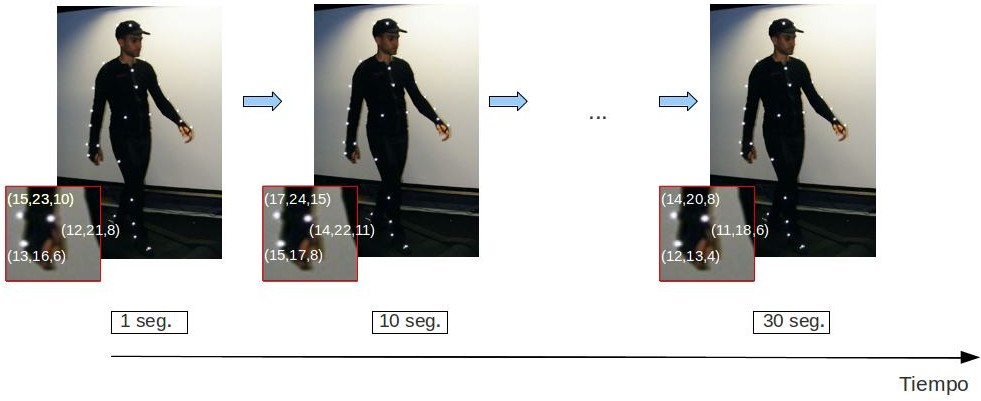
\includegraphics[scale=0.4]{img/Sistema_completo/diagrama_abuelas_2.jpg}
\end{center}
\caption{Posición de los marcadores a lo largo del tiempo.}
\label{abuela2}
\end{figure}

La aplicación recibe como entrada imágenes de video provenientes de varias cámaras, las cuales capturan el movimiento de una persona desde distintos ángulos. Se implementan métodos que permiten obtener información sobre las cámaras y su disposición en el espacio mediante la calibración. Con esta información y a partir de las imágenes obtenidas se detectan distintos puntos de referencia del cuerpo según el estudio particular que se desee realizar. Posteriormente, a partir de la información de las múltiples cámaras se reconstruye la posición 3D de los puntos en cada cuadro, para luego efectuar la identificación de trayectorias de los puntos de interés a lo largo de la secuencia, ver Figura \ref{abuela1}. A partir del procesamiento de la posición 3D de los puntos se obtendrán otros datos estadísticos de interés para el usuario.\\

\begin{figure}[ht!]
\begin{center}
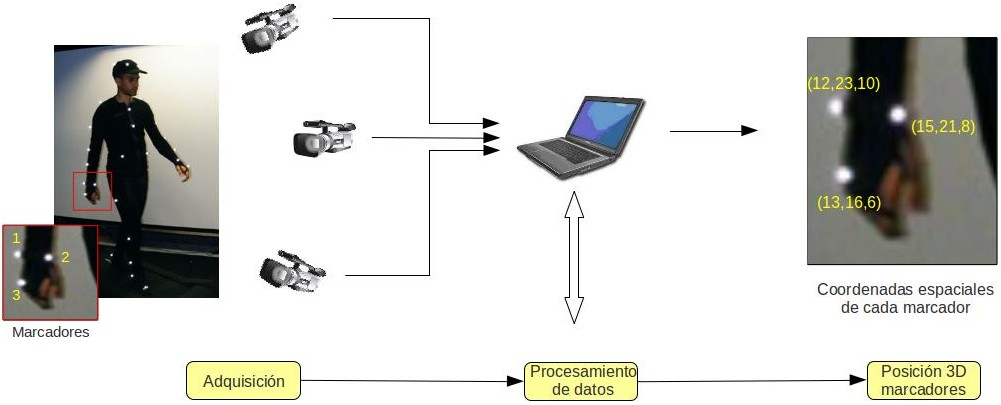
\includegraphics[scale=0.4]{img/Sistema_completo/diagrama_abuelas_1.jpg}
\end{center}
\caption{Funcionamiento de un sistema de captura de movimiento.}
\label{abuela1}
\end{figure}


%SINOPSIS
El proyecto se inicia con investigación y revisión bibliográfica sobre la temática, buscando diseños provenientes de sistemas de captura de movimiento ya implementados, así como  detalles sobre la implementación parcial o total de cada funcionalidad de interés. 
\\ 

Rápidamente se procuró obtener una base de datos con secuencias, ya sean reales o sintéticas, sobre los cuales implementar la aplicación y sus distintos bloques. Si bien esta búsqueda no aportó los resultados esperados,
%no obtuvo buenos resultados %ME QUERES MATAR ANDREI!!!!
 debido a que no se encontraron bases de datos acorde a las necesidades del proyecto, se implementa un prototipo de base de datos sintética con un número reducido de secuencias como alternativa tomando algunos conceptos encontrados en dicho relevamiento, generando una base flexible, de fácil expansión y con potencial para futuros estudios.\\ 

 Luego de analizar la bibliografía y definir la metodología, se opta por implementar el sistema con los 4 bloques principales mostrados en la Figura \ref{bloquesSistintro}. 

 \begin{figure}[H]
\begin{center}
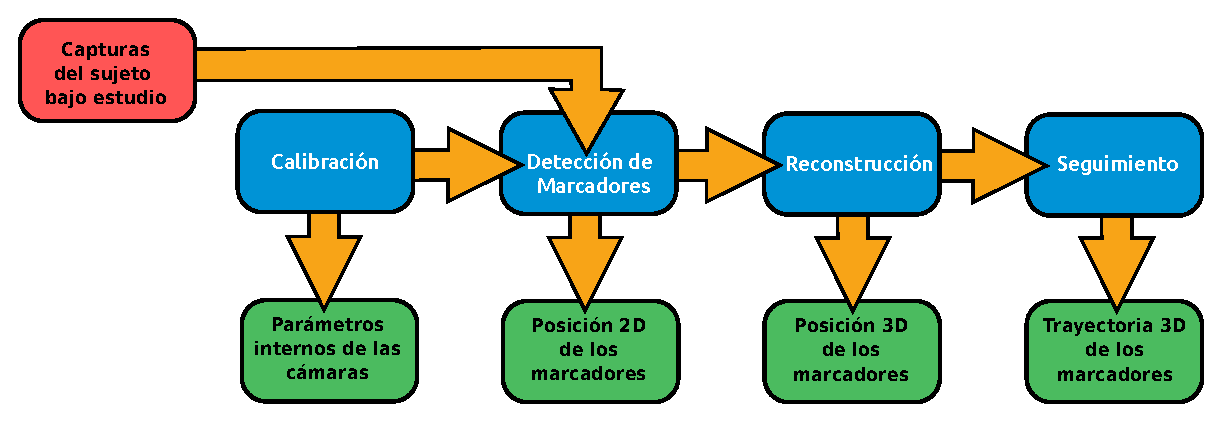
\includegraphics[scale=0.7]{img/Sistema_completo/Diagrama_de_bloques.eps}
\end{center}
\caption{Diagrama de bloques del sistema a implementar.}
\label{bloquesSistintro}
\end{figure}

Cada uno de estos bloques cumple un objetivo definido:
\begin{itemize}
\item El bloque de \emph{calibración}, es el encargado de obtener los parámetros internos y externos de las múltiples cámaras utilizadas en la captura, permitiendo establecer la relación entre el espacio ambiente y la imagen sobre cada cámara. Una vez que se disponen el número y posición de las cámaras para efectuar la captura de movimiento, este bloque releva por única vez la información previa necesaria para realizar una correcta reconstrucción de los puntos.
\item El bloque \emph{detección de marcadores}, identifica los marcadores en las imágenes obteniendo la posición 2D de cada uno de ellos a lo largo de la secuencia de captura en cada cámara (ver Figura \ref{peladocirculosintrointro}).
\item Con información de posición 2D proveniente de la detección de marcadores en múltiples vistas, y los parámetros relevados en calibración, el bloque de \emph{reconstrucción} (ver Figura \ref{peladoewconstruidointro}) se encarga de obtener la posición 3D de cada marcador.
\item Por último, el bloque de \emph{seguimiento} (ver Figura \ref{peladoetrackingintro})
(o ``tracking'') relaciona cada marcador en determinado cuadro de la secuencia con los que le siguen en el resto de los cuadros, obteniendo así la trayectoria de cada marcador a lo largo del tiempo.
\end{itemize}

Cabe destacar que estos bloques se implementaron de manera independiente, con una interfaz claramente definida, de manera  de poder realizar modificaciones sobre uno de ellos sin afectar el funcionamiento de los otros. Este aspecto cobra relevancia en etapas futuras, donde bajo la necesidad de optimizar algún bloque en particular o agregar alguna nueva característica que permita procesar datos provenientes de nuevos casos de uso, se deba modificar el sistema. De no presentar esta particularidad, la modificación de un bloque podría afectar negativamente el funcionamiento del sistema completo, requiriendo una posible re-ingeniería de la estructura.

\begin{figure}[ht!]
        \centering
        \hspace{1.3 cm}
        \subfloat[Captura original]{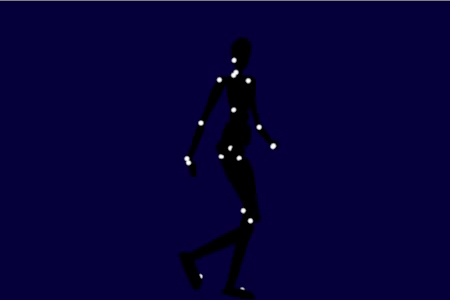
\includegraphics[scale=0.4]{img/peladoFondoAzul.png} %\label{peladoOriginalintrointro}
        }\hspace{2.2 cm}
        \subfloat[Detección de marcadores]{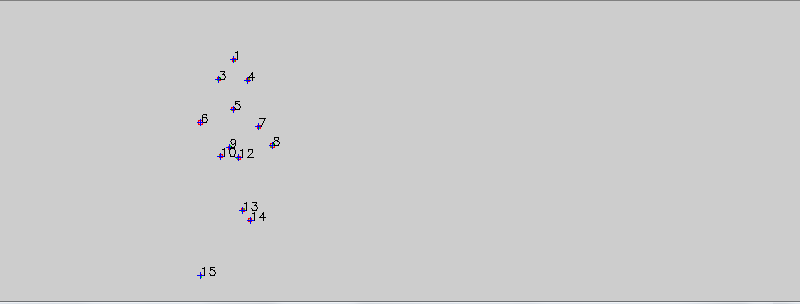
\includegraphics[scale=0.4]{img/peladoFondoAzul_circulos.png}\label{peladocirculosintrointro}}

        \subfloat[Recontrucción 3D]{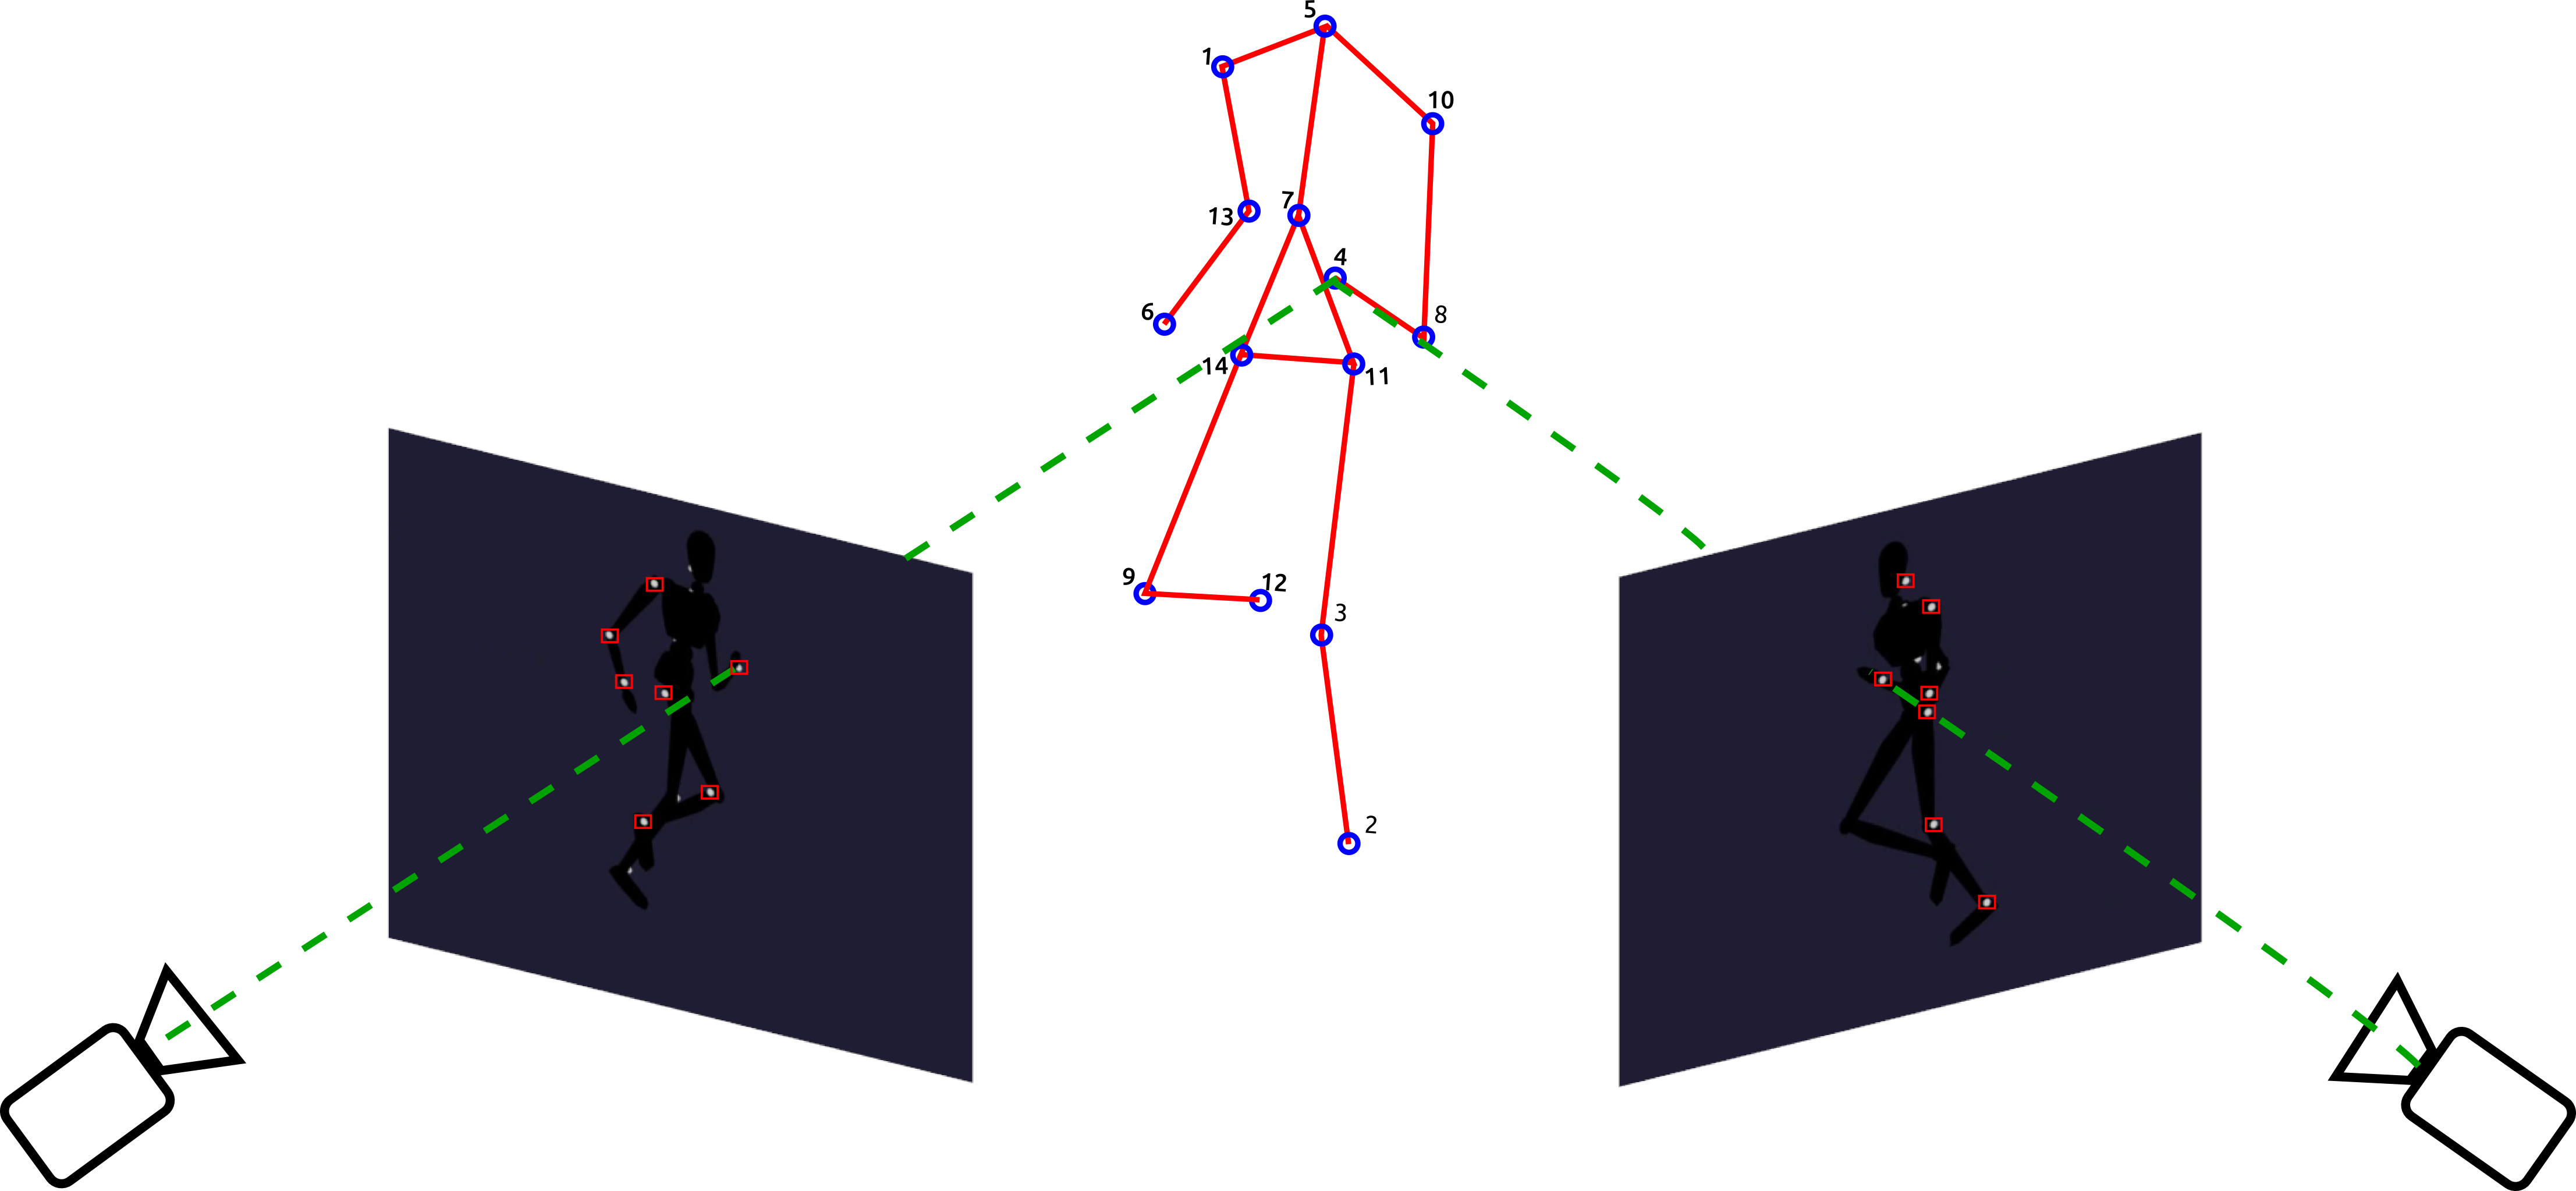
\includegraphics[scale=0.15]{img/Reconstruccion/reconstruccion1.png}\label{peladoewconstruidointro}}
    	\subfloat[Seguimiento]{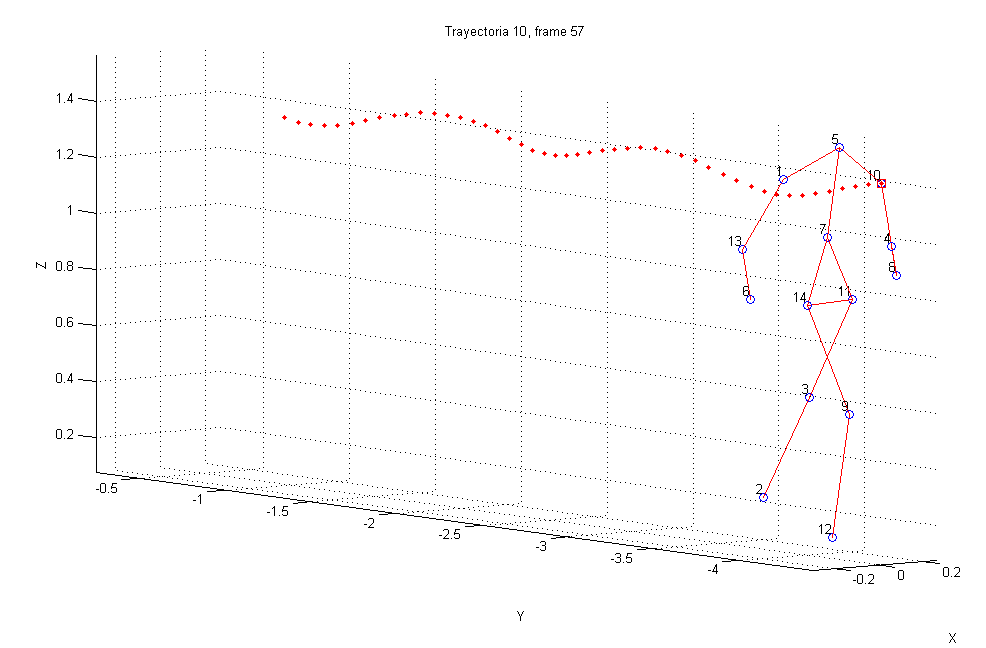
\includegraphics[scale=0.24]{img/Tracking/track1.png}\label{peladoetrackingintro}}  
  \caption{Salidas de los bloques principales del sistema.}
      \label{ejemplotutiintro}
\end{figure}

Por otro lado, fue elaborada una interfaz gráfica básica de forma tal de facilitar la ejecución del software para los usuarios sin tener que trabajar directamente con el código.
\\ 

A continuación se presenta una breve revisión del estado del arte de los sistemas de captura de movimiento disponibles. Una descripción más detallada y más técnica se realizará en la Sección \ref{invBiblio}, luego se define el objetivo del proyecto y se comenta la estructura de la documentación.

\section{Estado del arte}
%%%%%%%%%%%%%%%%%%%%%%%%%%%%%%%%%%%%%%%%%%%%%%%%%%%%%%%%%%%%%%%%%%%%%%%%%%%%%%%%%%%%%%%%%%%%%%%%%%%%%%%%%%%%%%%%%%%%%%%%%%%%%%%%%%%5
%qué opciones tengo para hacerlo? por qué hay estas opciones? para qué se usan?
%%%%%%%%%%%%%%%%%%%%%%%%%%%%%%%%%%%%%%%%%%%%%%%%%%%%%%%%%%%%%%%%%%%%%%%%%%%%%%%%%%%%%%%%%%%%%%%%%%%%%%%%%%%%%%%%%%%%%%%%%%%%%%%%%%%

Al día de hoy existen varios sistemas de captura de movimiento, sin embargo los mas usados debido a su buena performance y soporte presentan altos costos de licenciamiento. 
\\ 

Como se mencionó anteriormente, los más populares en la actualidad son los que se utilizan en la industria del cine o del diseño de videojuegos. En este contexto, se almacenan las acciones de actores humanos y se usa esta información para animar modelos digitales de personajes en animación 3D.
\\ 

Algunos ejemplos de sistemas de captura de movimiento bajo licencia son:

\begin{itemize}
\item \emph{Vicon} \cite{vicon}. Es una empresa que vende sistemas de captura de movimiento, tanto software como hardware. Sus sistemas son muy conocidos y fuertemente utilizados en estudios clínicos y biomecánicos alrededor del mundo, así como para otras investigaciones científicas. En particular, este sistema está siendo utilizado en el Departamento de Fisiatría y Rehabilitación del Hospital de Clínicas. Presenta como ventajas frente a otros sistemas la velocidad con que realiza el procesamiento de los datos y la calidad de las cámaras para realizar las capturas. La gran desventaja que posee es el alto costo de sus equipamientos, bastante privativo en algunos ámbitos.
\item \emph{Qualisys} \cite{qualisys}. Junto con Vicon son los dos sistemas de captura de movimiento más utilizados en el ámbito de la investigación científica. Presenta como ventajas frente al anterior la utilización del modelo AIM\footnote{Automatic Identification of Markers}, un identificador de marcadores que ``aprende'' de cada secuencia procesada ahorrando mucho tiempo y trabajo en identificar marcadores. Además presenta una interfaz de usuario más amigable y requiere menos tiempo de capacitación para su uso.
\item \emph{OptiTrack} \cite{optitrack}. Es de los sistemas comerciales de menor costo, cerca de la cuarta parte de lo que cuesta un sistema Vicon. Otra de sus ventajas es que brinda acceso de bajo nivel a través de un conjunto de  SDK's y API's tanto para el hardware como para los datos obtenidos, permitiendo manipular los mismos y procesarlos de la manera deseada por fuera de las aplicaciones que originalmente provee. 
\item \emph{Massive} \cite{massive}. Es un software destinado a producir efectos especiales para cinematografía, programas televisivos y videojuegos entre otras cosas. El software implementa la captura de movimiento y cuenta con varios productos para generar distintos tipos de efectos y animaciones. Fue originalmente diseñado par utilizar en la trilogía de El Señor De Los Anillos de Peter Jackson y desde entonces se ha convertido en uno de los mejores software para realizar efectos visuales de muchedumbres y animación de personajes autónomos.
\item \emph{Motion Analysis} \cite{motion_analysis}. es el mayor fabricante mundial de sistemas de instrumentación óptica de alto rendimiento que permite testear y medir el movimiento de los objetos. Mantiene y comercializa el software con sus sistemas de hardware. Sus sistemas evalúan el movimiento en distintas aplicaciones: producción de animación, análisis de movimiento, y en el ámbito industrial. Posee un gran número de aplicaciones de pos-producción.

\item \emph{PhaseSpace} \cite{phasespace}. Posee un sistema de captura patentado basado en marcadores leds, de alta resolución temporal y espacial. Todo el sistema se compone de sólo unos pocos elementos robustos y portátiles. Sus aplicaciones funcionan tanto en entornos Linux como Windows. Ha desarrollado soluciones de captura de movimiento para la investigación, la industria y las comunidades de las artes gráficas, también para estar al alcance de las pequeñas empresas, universidades y particulares.
\end{itemize}

Los sistemas anteriores, y la mayoría de los sistemas modernos que efectúan capturas de movimiento, utilizan sensores infrarrojos o LEDs para efectuar el seguimiento de puntos. Los segundos facilitan la etapa de detección de marcadores en cada cámara, mientras que los primeros no tienen una etapa de detección en cada vista ni reconstrucción ya que los mismos ofrecen la información de posición directamente.
\\ 

La gran desventaja de los sistemas anteriores es su alto costo. A modo de ejemplo, un sistema Vicon de 10 cámaras tiene un valor que ronda los U\$S\;70.000 \footnote{Este precio depende fuertemente del tipo de cámara que se utilice, los precios de las mismas se encuentran a partir de los U\$S\;3.000 por unidad.}.
\\ 


Por otro lado, también existen programas de captura de movimiento de código libre, un ejemplo de ello es el programa Kinovea \cite{kinovea}. Enfocado principalmente en el ámbito deportivo, permite analizar y mejorar la técnica de los atletas a través del procesamiento de secuencias de video. Posee algunas características interesantes como la posibilidad de efectuar medición de distancias, ángulos y tiempos manualmente, así como la utilización de seguimiento semi-automático de puntos en tiempo real para obtener su trayectoria. La gran desventaja que presenta frente a otros sistemas es que efectúa únicamente análisis sobre dos dimensiones y con una sola cámara.\\

Otra alternativa sobre la que se investigó es DVIDEOW \cite{figueroa2003flexible}. Este software presenta varios conceptos teóricos como primer acercamiento al problema, pero la implementación presenta pérdidas de marcadores que requieren correcciones constantes. Además, no se tiene una actualización del mismo desde el 2009, desde esa fecha a la actualidad solamente se encontraron trabajos que lo presentan como fundamento teórico.

\section{Estructura de la documentación}

Este proyecto estudia el problema de captura de movimiento y sus distintas componentes, para desarrollar un conjunto de datos y presentar un análisis sobre los mismos. 
\\

En este capitulo se presentó el objetivo general del proyecto y un breve estado del arte de la temática que será desarrollado profundamente en el Capítulo~\ref{invBiblio}, junto a un planteo en la Figura~\ref{bloquesSistintro} de los bloques que se estudiarán a lo largo del proyecto. 
\\

El Capítulo~\ref{section_base_de_datos} presentará un estudio de bases de datos disponibles y como fueron generadas capturas experimentales propias sobre las cuales trabajar. Luego el Capítulo~\ref{sec:implementacion_bloques_sistema} presentará detalles sobre el procedimiento de la Figura~\ref{bloquesSistintro} a partir de los datos experimentales generados. 
\\

En los capítulos siguientes se presentará como fue estudiado e implementado cada bloque: Segmentación y Filtrado en el Capítulo~\ref{deteccionMarcadoresSec} para la detección de la posición de los marcadores en cada video, Calibración en el Capítulo~\ref{calibracion} donde se mostrará como se genera la información del espacio de captura necesaria para luego en el Capítulo~\ref{reconstruccion} sobre Reconstrucción, mostrar como se combina la información de los bloques anteriores para calcular la posición en el espacio de los marcadores. 
\\

Posteriormente, el Capítulo~\ref{seguimiento} sobre Seguimiento propone un método de identificación de marcadores reconstruidos. 
\\

Finalmente se presenta como fue evaluado cada bloque y múltiples pruebas sobre el sistema completo en el Capítulo~\ref{evaluacion} para luego presentar las conclusiones en el Capítulo~\ref{conclusiones}.


 
  


%Dada las características de este proyecto otro antecedente relevante a tener en cuenta en el área, es el de un grupo de investigadores del Hospital de Clínicas que junto al grupo de Tratamiento de Imágenes de la Facultad de Ingeniería han estudiado previamente la marcha de las personas a los efectos de reconocer en ellas patrones de movimiento. Dicho proyecto recibe el nombre “Cíclope”.

\chapter{Implementación de bloques del sistema}
\label{sec:implementacion_bloques_sistema}

%COMENTARIO: ACÁ SE ME OCURRE DE HACER UNA INTRODUCCIÓN A CADA BLOQUE DEL SISTEMA, JUSTIFICAR Y EXPLICAR MEDIO POR ARRIBA Y EN LAS SIGUIENTES SECCIONES EXPLICAR LOS DETALLES MÁS TÉCNICOS DE CADA BLOQUE.

En base a lo estudiado en la etapa de investigación, se pudo concluir que un sistema de captura de movimiento con las características necesarias para cumplir el objetivo del proyecto debe estar formado por 4 bloques generales: \emph{calibración}, \emph{detección de marcadores}, \emph{reconstrucción} y \emph{seguimiento}. En la figura \ref{bloquesSist} se muestra un esquema del sistema a implementar.

\begin{figure}[H]
\hspace{-0.5cm}
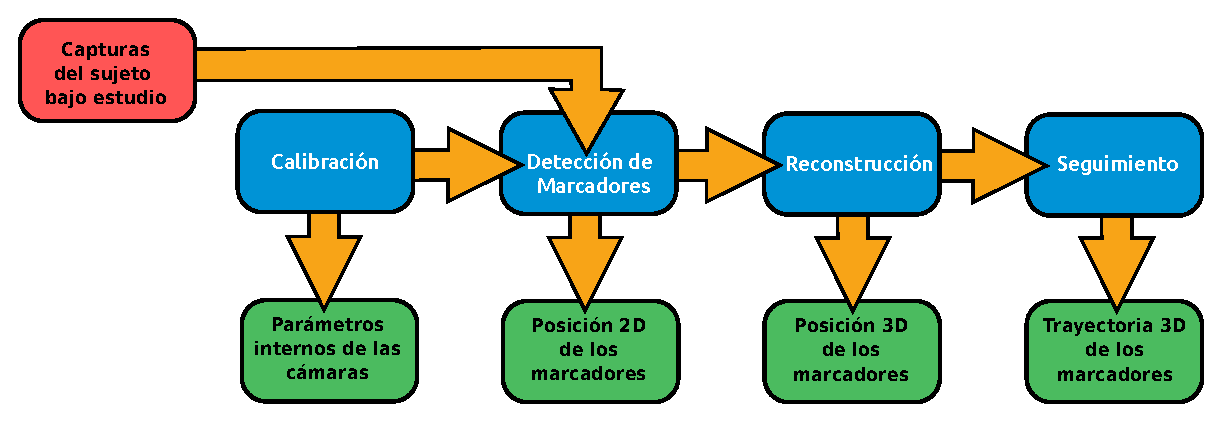
\includegraphics[scale=0.7]{img/Sistema_completo/Diagrama_de_bloques.eps}
\caption{Diagrama de bloques del sistema completo.}
\label{bloquesSist}
\end{figure}

A grandes rasgos, el sistema funciona de la siguiente manera:

\begin{enumerate}
	\item Se \emph{calibran} las cámaras. Esto es, determinar los parámetros de las mismas de forma tal de tener un mapeo del espacio 3D a las coordenadas 2D de las imágenes capturadas.
	\item Se realiza la captura del paciente en movimiento desde todas las cámaras calibradas.
	\item A partir de las secuencias, se realiza la \emph{detección de marcadores} para cada cámara. Esto equivale a determinar la posición 2D de dichos marcadores en cada cámara donde están visibles, a lo largo de toda la secuencia.
	\item Luego, con la posición 2D de determinado marcador en al menos 2 cámaras se realiza la \emph{reconstrucción} del mismo, es decir, obtener las coordenadas 3D de dicho marcador. Se realiza para todos los marcadores, y para todos los cuadros de la secuencia.
	\item Finalmente, se realiza el \emph{seguimiento} (o \emph{tracking}) de cada marcador en el espacio. Con esto se obtienen las trayectorias 3D de todos los marcadores en el cuerpo del paciente.
\end{enumerate}

Debido a los tiempos disponibles para realizar el proyecto en su totalidad, y junto a la planificación realizada al comienzo del mismo, se tiene como idea principal el conseguir la implementación de un sistema con características similares, adaptando el mismo para cumplir los objetivos establecidos. 

Sin embargo en la investigación bibliográfica se encuentra otra realidad, puesto que no hay muchos sistemas a disposición. Por un lado, la mayor parte de los sistemas encontrados poseen altos costos de licenciamiento (por ejemplo Vicon\footnote{http://www.vicon.com/, Noviembre 2014}, OptiTrack\footnote{http://www.naturalpoint.com/optitrack/, Noviembre 2014}, PhaseSpace\footnote{http://www.phasespace.com/index.html, Noviembre 2014}, Qualisys\footnote{http://www.qualisys.com/, Noviembre 2014} o MotionAnalysis\footnote{http://www.motionanalysis.com/index.html, Noviembre 2014}) y por otro lado, los sistemas de código abierto no se adaptaban a las necesidades presentes o el trabajo a realizar sobre los mismos era más Costoso que hacer una implementación propia. En este último caso se encuentra el software Kinovea\footnote{http://www.kinovea.org/, Noviembre 2014}, que realiza únicamente el seguimiento en coordenadas 2D.

Debido a los inconvenientes planteados, se decide realizar una implementación propia de los bloques del sistema. Nuevamente, de acuerdo a la filosofía explicada en los párrafos anteriores, se prioriza la búsqueda de sistemas ya implementados cuyo diseño se corresponda a cada bloque de la Figura \ref{bloquesSist},  antes de recurrir a la creación de uno.

Se tuvo presente en esta búsqueda el hecho de poder separar el sistema en bloques independientes. Esto asegura que la construcción de uno de ellos no dependa del correcto funcionamiento de otro. Por otro lado, da la posibilidad que en etapas futuras se pueda realizar el estudio de uno de los bloques de la Figura \ref{bloquesSist} individualmente y así poder modificarlo u optimizarlo sin afectar al resto. Esta forma de trabajo funciona adecuadamente siempre y cuando la salida de un bloque sea exactamente la entrada del siguiente, para los casos en que no se logra esto, se realizan algoritmos capaces de importar la salida de un bloque y convertirla al formato de entrada de otro (por ejemplo, \textit{Xml2Struct} que convierte el xml que tiene como salida el bloque de detección de marcadores en estructuras de Matlab para realizar la reconstrucción).

Como se menciona anteriormente, en la búsqueda realizada se encuentra la tesis de doctorado de Lorna Herda\cite{herda}, la misma plantea un sistema de captura de movimiento con las características buscadas para este proyecto. Al estudiar dicho sistema se encuentra que posee las mismas hipótesis de uso que el estudio preliminar realizado (utilización en fisioterapia, biomecánica, animación, deporte, etc.). Además, es un trabajo mencionado repetidas veces en otros artículos de la misma rama científica, encontrándose una documentación amplia respecto a la metodología implementada.

Debido a las ventajas que presenta esta metodología respecto a las otras encontradas, se decide implementar el sistema de Herda y elaborar los bloques de calibración y detección de marcadores aparte.

Estudiado el diseño propuesto por Herda para su sistema, se construye un diagrama de bloques completo, más detallado que el mostrado en la Figura \ref{bloquesSist}, el cual se puede observar en la Figura \ref{diagBloq}. Es importante destacar que, si bien la mayor parte de los bloques de reconstrucción y seguimiento se realizaron con la metodología del sistema de Lorna Herda\cite{herda}, en la documentación se presentan ciertas ambigüedades respecto a la descripción de algunos métodos y en la forma de resolver determinados casos de uso, que tuvieron que ser analizados y definidos por el grupo del proyecto en base a los conocimientos adquiridos.

A continuación se muestra el diagrama de bloques y se explica su funcionamiento.

\section{Diagrama de bloques}

\vspace{-0.5cm}
\begin{figure}[ht!]
\hspace{-1cm}
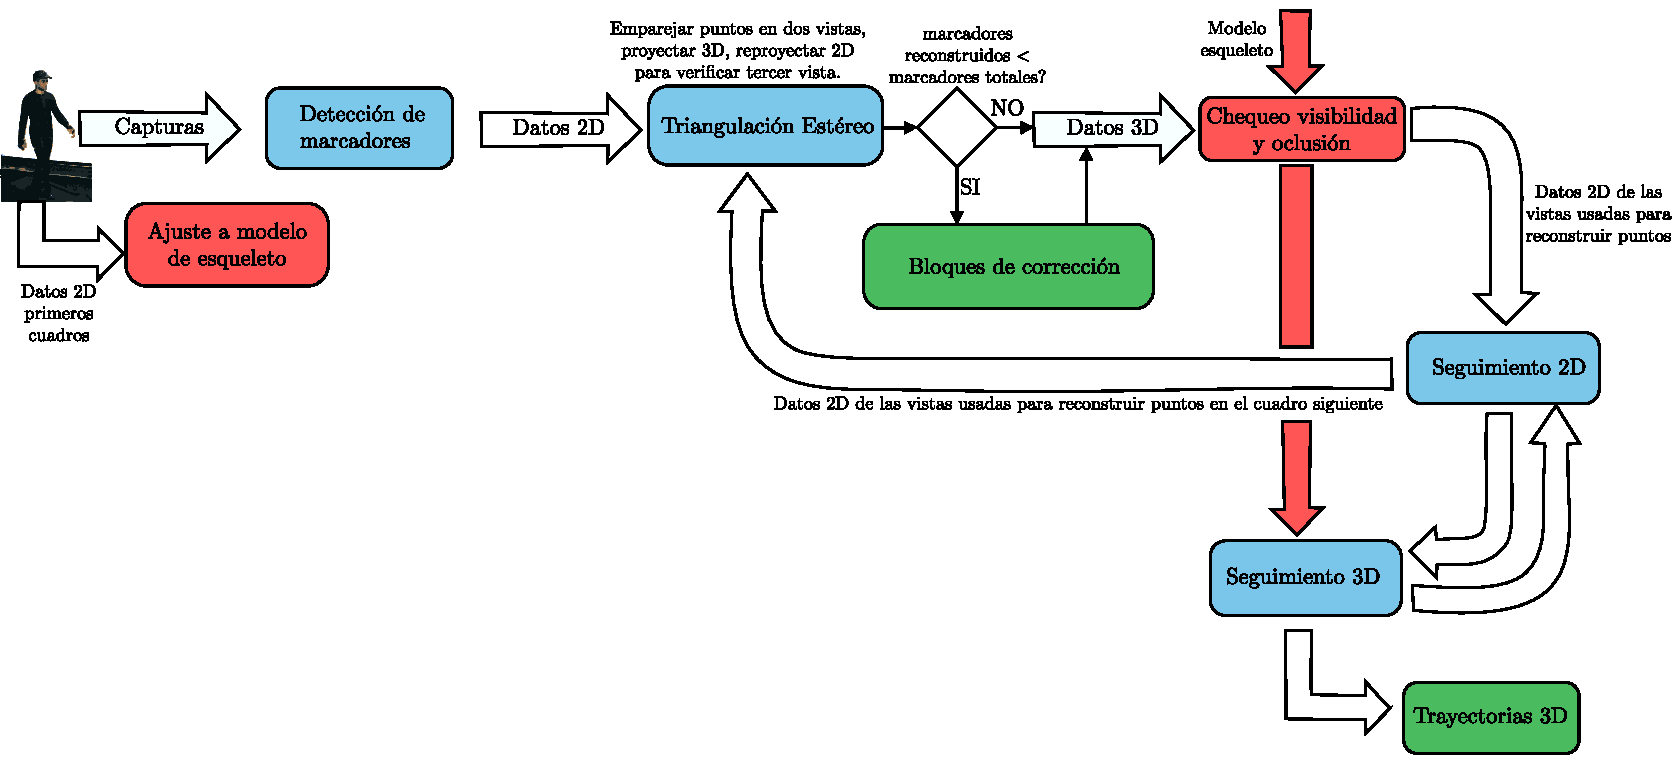
\includegraphics[scale=0.55]{img/Sistema_completo/Diagramadebloques_Herda.pdf}
\vspace{-1cm}
\caption{Diagrama de bloques detallado del sistema.}
\label{diagBloq}
\end{figure}

El sistema representado en este diagrama, funciona de la siguiente manera:

\begin{enumerate}
\item Se realiza la captura de movimiento del paciente desde múltiples vistas, en un entorno controlado. Estas capturas son la entrada principal al sistema.
\item A partir de las capturas, por un lado se ajusta el \textbf{modelo teórico de esqueleto} a utilizar, de acuerdo a las características del cuerpo del paciente, y por otro lado se realiza la \textbf{detección de marcadores} de cada cuadro para cada cámara. Este bloque es el mismo que el del diagrama de la figura \ref{bloquesSist} y se explicará en detalle en el Capítulo \ref{deteccionMarcadoresSec}.
\item Luego que se tiene la posición 2D de los marcadores en cada cuadro y en cada cámara, se realiza la \textbf{triangulación estéreo} para obtener la posición 3D de los mismos. A grandes rasgos, la \emph{triangulación 3D} empareja dos puntos en correspondencia de dos vistas distintas y con ellos calcula la proyección 3D de ese punto en el espacio, luego se re-proyecta ese punto en las otras vistas para verificar. Si verifica su posición en al menos una vista más, entonces la posición 3D se considera válida.
\item Si el número de marcadores reconstruidos en 3D es menor al número total de marcadores en el modelo de captura, se ingresa en el \textbf{bloque de corrección}, donde se utilizan varios métodos para recuperar la posición 3D de los marcadores restantes (ver Figura \ref{fig:bloqCorr}). 
\item Cuando se tiene la posición 3D de todos los marcadores, se ingresa en el bloque de \textbf{chequeo de visibilidad y oclusión} donde se verifica que la posición reconstruida de cada marcador sea correcta y no se haya reconstruido alguno con datos erróneos.
\item Finalmente, se realiza el \textbf{tracking 3D y 2D} en simultáneo para reconstruir las trayectorias de cada marcador.
\end{enumerate}

La explicación detallada de cada bloque y cómo fueron implementados se muestra en los capítulos siguientes.

A continuación, se explica como funciona el bloque de corrección:

\begin{figure}[H]
\hspace{-1cm}
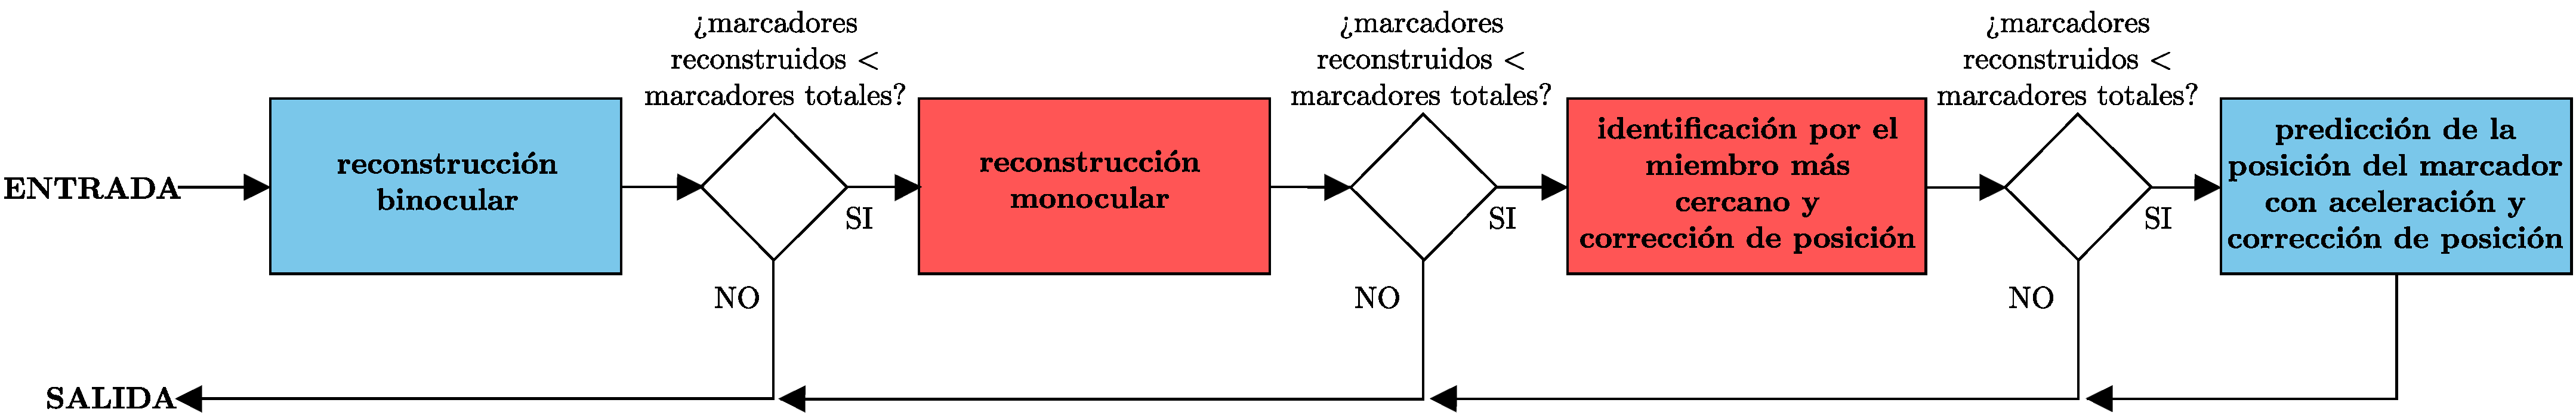
\includegraphics[scale=0.22]{img/Sistema_completo/BloquesDeCorreccion}
\caption{Detalle del bloque de corrección.}
\label{fig:bloqCorr}
\end{figure}

Una vez realizada la triangulación estéreo, se verifica que el número de marcadores reconstruidos sea igual a la cantidad de marcadores que efectivamente se estén usando en la adquisición de datos. Si esta condición no se verifica, se ejecuta un “bloque de corrección” para solucionarlo. Dicho bloque a su vez, contiene  varios sub-bloques, los cuales pueden verse en la figura \ref{fig:bloqCorr}.

Primeramente se efectúa la \emph{reconstrucción binocular} y si aún no se obtienen todos los marcadores se efectúa la \emph{reconstrucción monocular}, se disminuye la exigencia sobre la reconstrucción al utilizar sucesivamente métodos menos precisos, con el fin de completar el número de \emph{marcadores reconstruidos}.

 Si en la salida de cada uno de los bloques anteriores la condición de \emph{todos los marcadores reconstruidos} aún no se cumple, se pasa al siguiente bloque, donde se asocian los marcadores 3D reconstruidos que aún no fueron identificados con aquellas articulaciones del modelo de esqueleto (ajustado en la inicialización) que no tienen ningún marcador asociado. Para esto, se evalúan las distancias de los marcadores no identificados con la posición de las articulaciones del modelo en cuadros anteriores y se asocian aquellos marcadores que se encuentren a menor distancia a cada una de dichas articulaciones. Al tiempo que se realiza esto, se verifica que la distancia entre marcadores asociados a un mismo hueso del esqueleto se mantenga aproximadamente constante (dado que los marcadores están fijos en los huesos y los mismos no varían su tamaño).
 
Si aún faltan marcadores sin reconstruirse, se utiliza como último recurso la estimación de la posición del marcador evaluando la aceleración del mismo en cuadros anteriores y verificando que dicha estimación sea coherente con el modelo de esqueleto.



Si bien se intentó reproducir el sistema propuesto por Herda\cite{herda} tal cual se especificaba en su documentación, se presentaron diversos obstáculos que impidieron poder implementar los bloques de reconstrucción y seguimiento como se detalló anteriormente. El principal obstáculo fue el calendario, ya que la cantidad de módulos a implementar es demasiado grande para el tiempo con que cuenta este proyecto. Otro factor importante que influyó son las ambigüedades presentadas en las especificaciones de los bloques en la documentación de Herda, dado que retrasaron la etapa de estudio del sistema al tener que investigar e implementar métodos para poder superar los vacíos presentes en la teoría.

 A raíz de esto, se decide darle prioridad a los bloques principales del diagrama frente a los secundarios o a los que se implementan para casos de uso particulares. Con esto se intenta tener implementado un sistema de principio a fin, capaz de capturar la posición 3D de un sujeto realizando el movimiento de marcha a lo largo del tiempo. Estos bloques son:
 \begin{itemize}
 	\item Detección de marcadores
 	\item Triangulación estéreo (Reconstrucción)
 	\item Seguimiento 3D
 	\item Calibración
 \end{itemize}

En los capítulos que siguen, se explicará el funcionamiento de estos bloques de forma detallada, así como su implementación y el análisis de resultados de cada uno de ellos.

\subsection{Markers Detection}
Markers detection block, can be divided in two parts: \textit{segmentation} and \textit{objects filter}.
%
Algorithm makes the detection through the following process:
%
\begin{enumerate}
  \item Get each frame from video input.
  \item Take a frame and segment it using Otsu's threshold.
  \item Detect markers from segmented image.
  \item Write detected markers position in an XML file.
  %\item Se escribe la posición de los marcadores detectados para este cuadro en un archivo con formato XML.
  \item Take the following frame and repeat process from step two.
\end{enumerate}
%
\subsubsection{Detection stages description}
\textit{Segmentation} block uses thresholds with three class Otsu's method\cite{otsu}.\\
%
\textit{Filtering} stage is just a classification of segmented objects. Since objects to be detected have relatively simple shapes (white circles on dark background) and laboratory conditions are controlled during the capture, this stage not required to implement a complex algorithm. Particularly, it was implemented a circular object detector based on geometric moments\cite{imageMoments} and an area based filter.
%
\subsubsection{Results}
It was observed that results on segmentation stage strongly depends from capture conditions and calculated threshold. Special care must be taken in capture conditions since if not meet the established, results are not entirely satisfactory.
On the other hand, if captures are made in the established conditions, obtained results are acceptable (Figure \ref{ejemploabelumbr2}).
\vspace{-0.5cm}
\begin{figure}[ht!]
      \centering
        {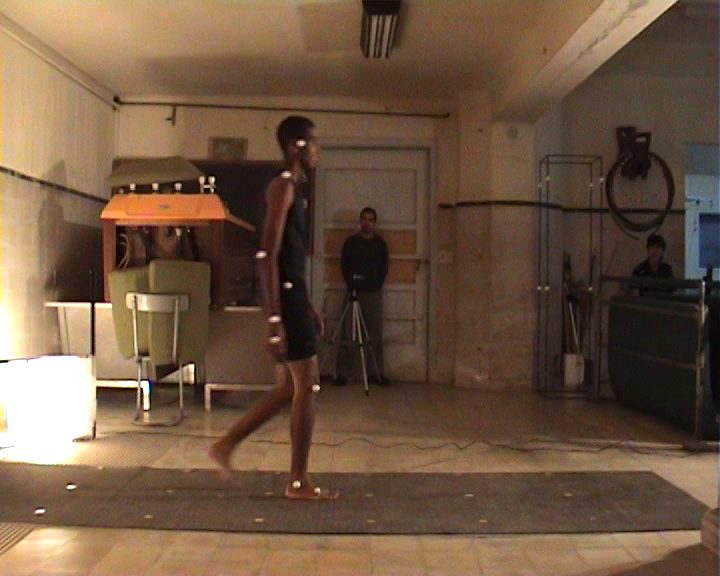
\includegraphics[scale=0.10]{imagenes/abel_original_video.png}\label{abelvideo}}\hspace{1 mm}
        {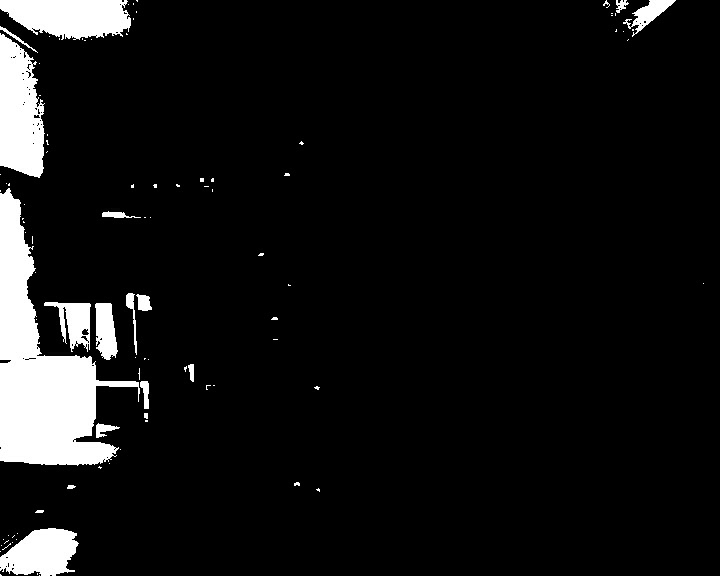
\includegraphics[scale=0.10]{imagenes/abel_original_filtro.png}\label{abelfiltro}}
        {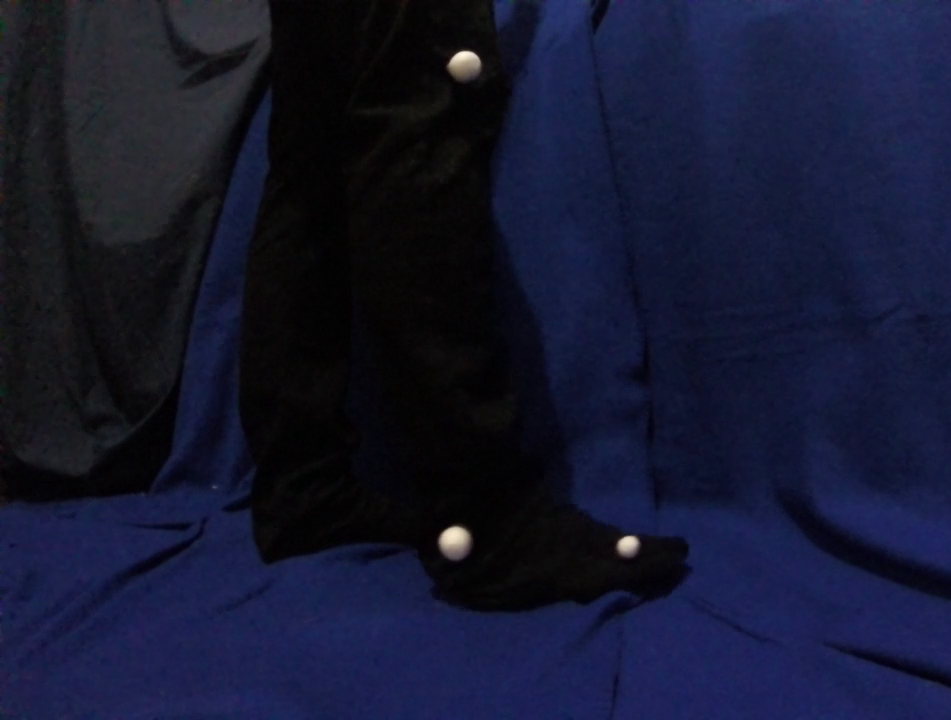
\includegraphics[scale=0.07]{imagenes/orig.png}\label{abelvideo2}}\hspace{1 mm}
       % {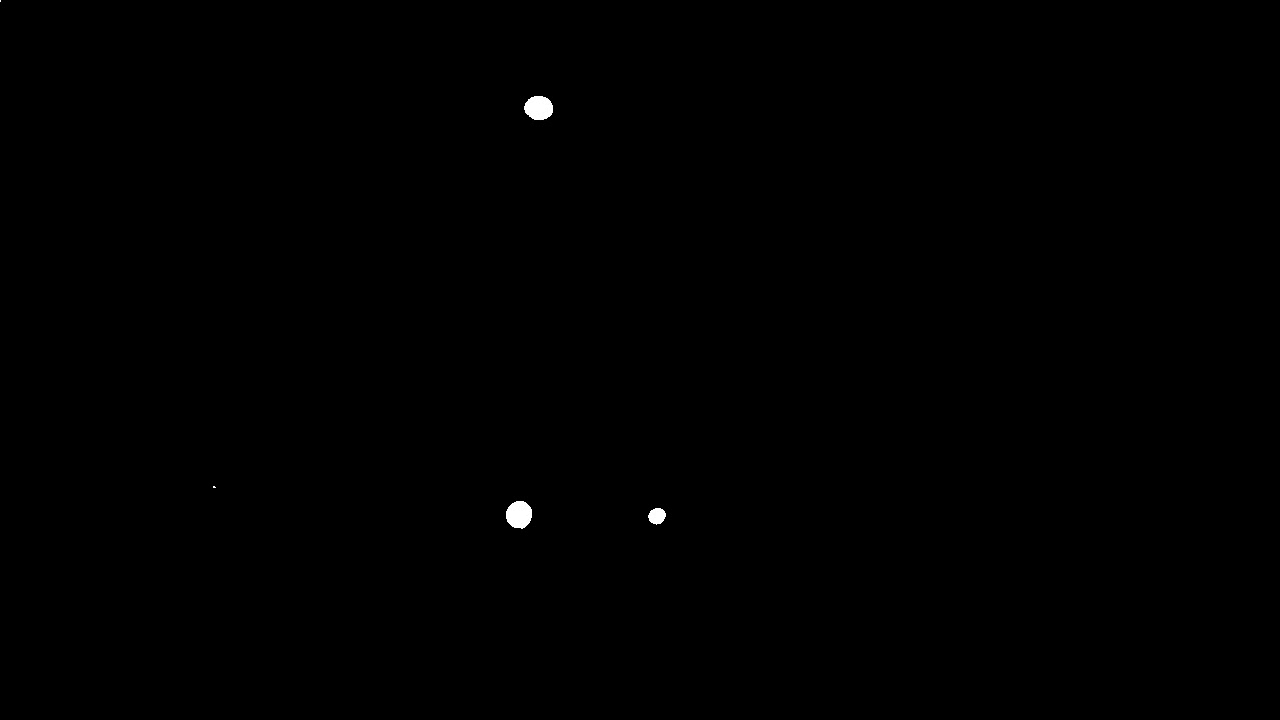
\includegraphics[scale=0.07]{imagenes/filtr.png}\label{abelfiltro2}}\hspace{1 mm}
        {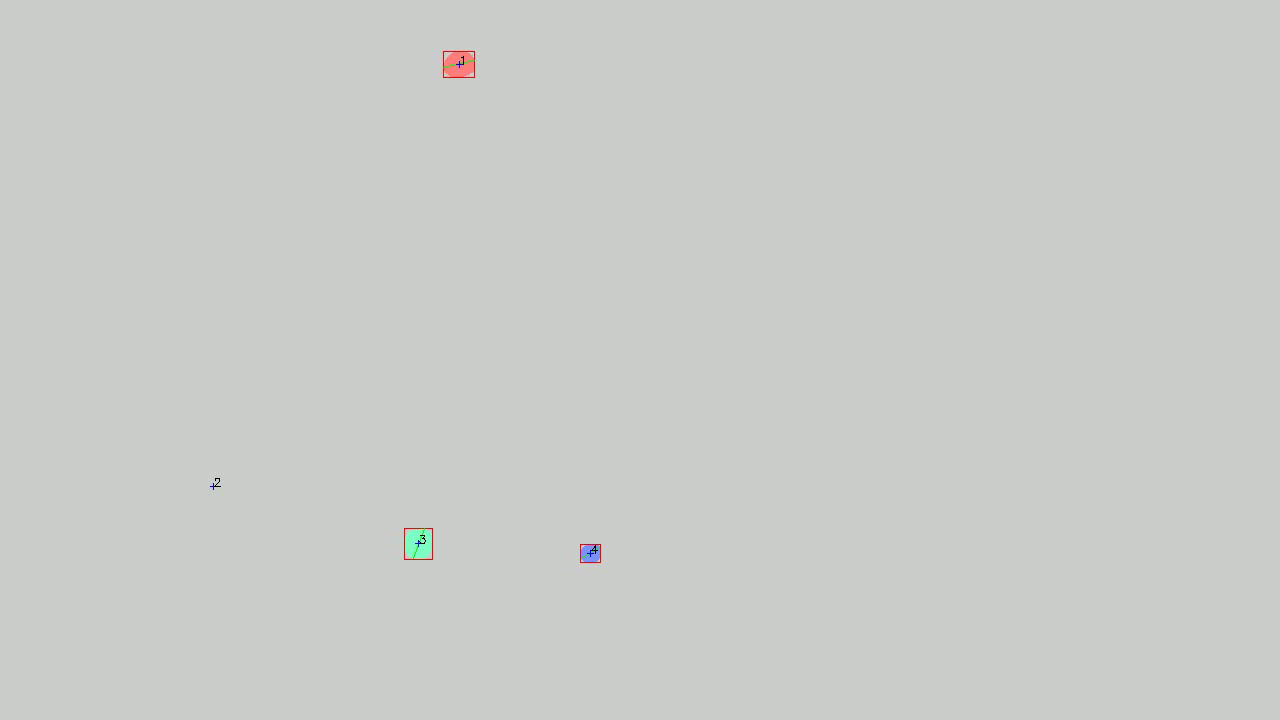
\includegraphics[scale=0.07]{imagenes/detect.png}
        \label{abeldetect}}
      \caption{%Entradas y salidas de cada etapa del bloque de deteción.
       %\textbf{(\ref{abelvideo})} 
       \textit{Left}: original image from a sequencue without capture hypothesis. 
       \textit{Left center}: segmentation results without capture hypothesis.
       % \textbf{(\ref{abelvideo2})} 
       \textit{Right center}: Original capture from a real sequence under capture hypothesis.
       % \textbf{(\ref{abelfiltro2})} Imagen filtrada con el umbral de Otsu. \textbf{(\ref{abeldetect})}
       \textit{Right}: Detected markers.}  
      \label{ejemploabelumbr2}
\end{figure}
%\vspace{-0.6cm}

\chapter{Reconstrucción}\label{reconstruccion}

\section{Introducción}
A la salida del bloque de detección de marcadores se tiene, para cada cámara y para cada cuadro de una secuencia adquirida, un conjunto de coordenadas en dos dimensiones $(x,y)$ que ubican la posición en la imagen de aquellos marcadores que fueron detectados.
El proceso de reconstrucción consiste en obtener las coordenadas en tres dimensiones de la posición de los marcadores en el espacio a partir de las coordenadas en dos dimensiones obtenidas en el bloque anterior.
En la Figura \ref{fig: esquema_reconstruccion} se muestra un bosquejo de la reconstrucción de un marcador usando para esto la detección de marcadores en dos cámaras.\\

\begin{figure}[ht!]
\begin{center}
%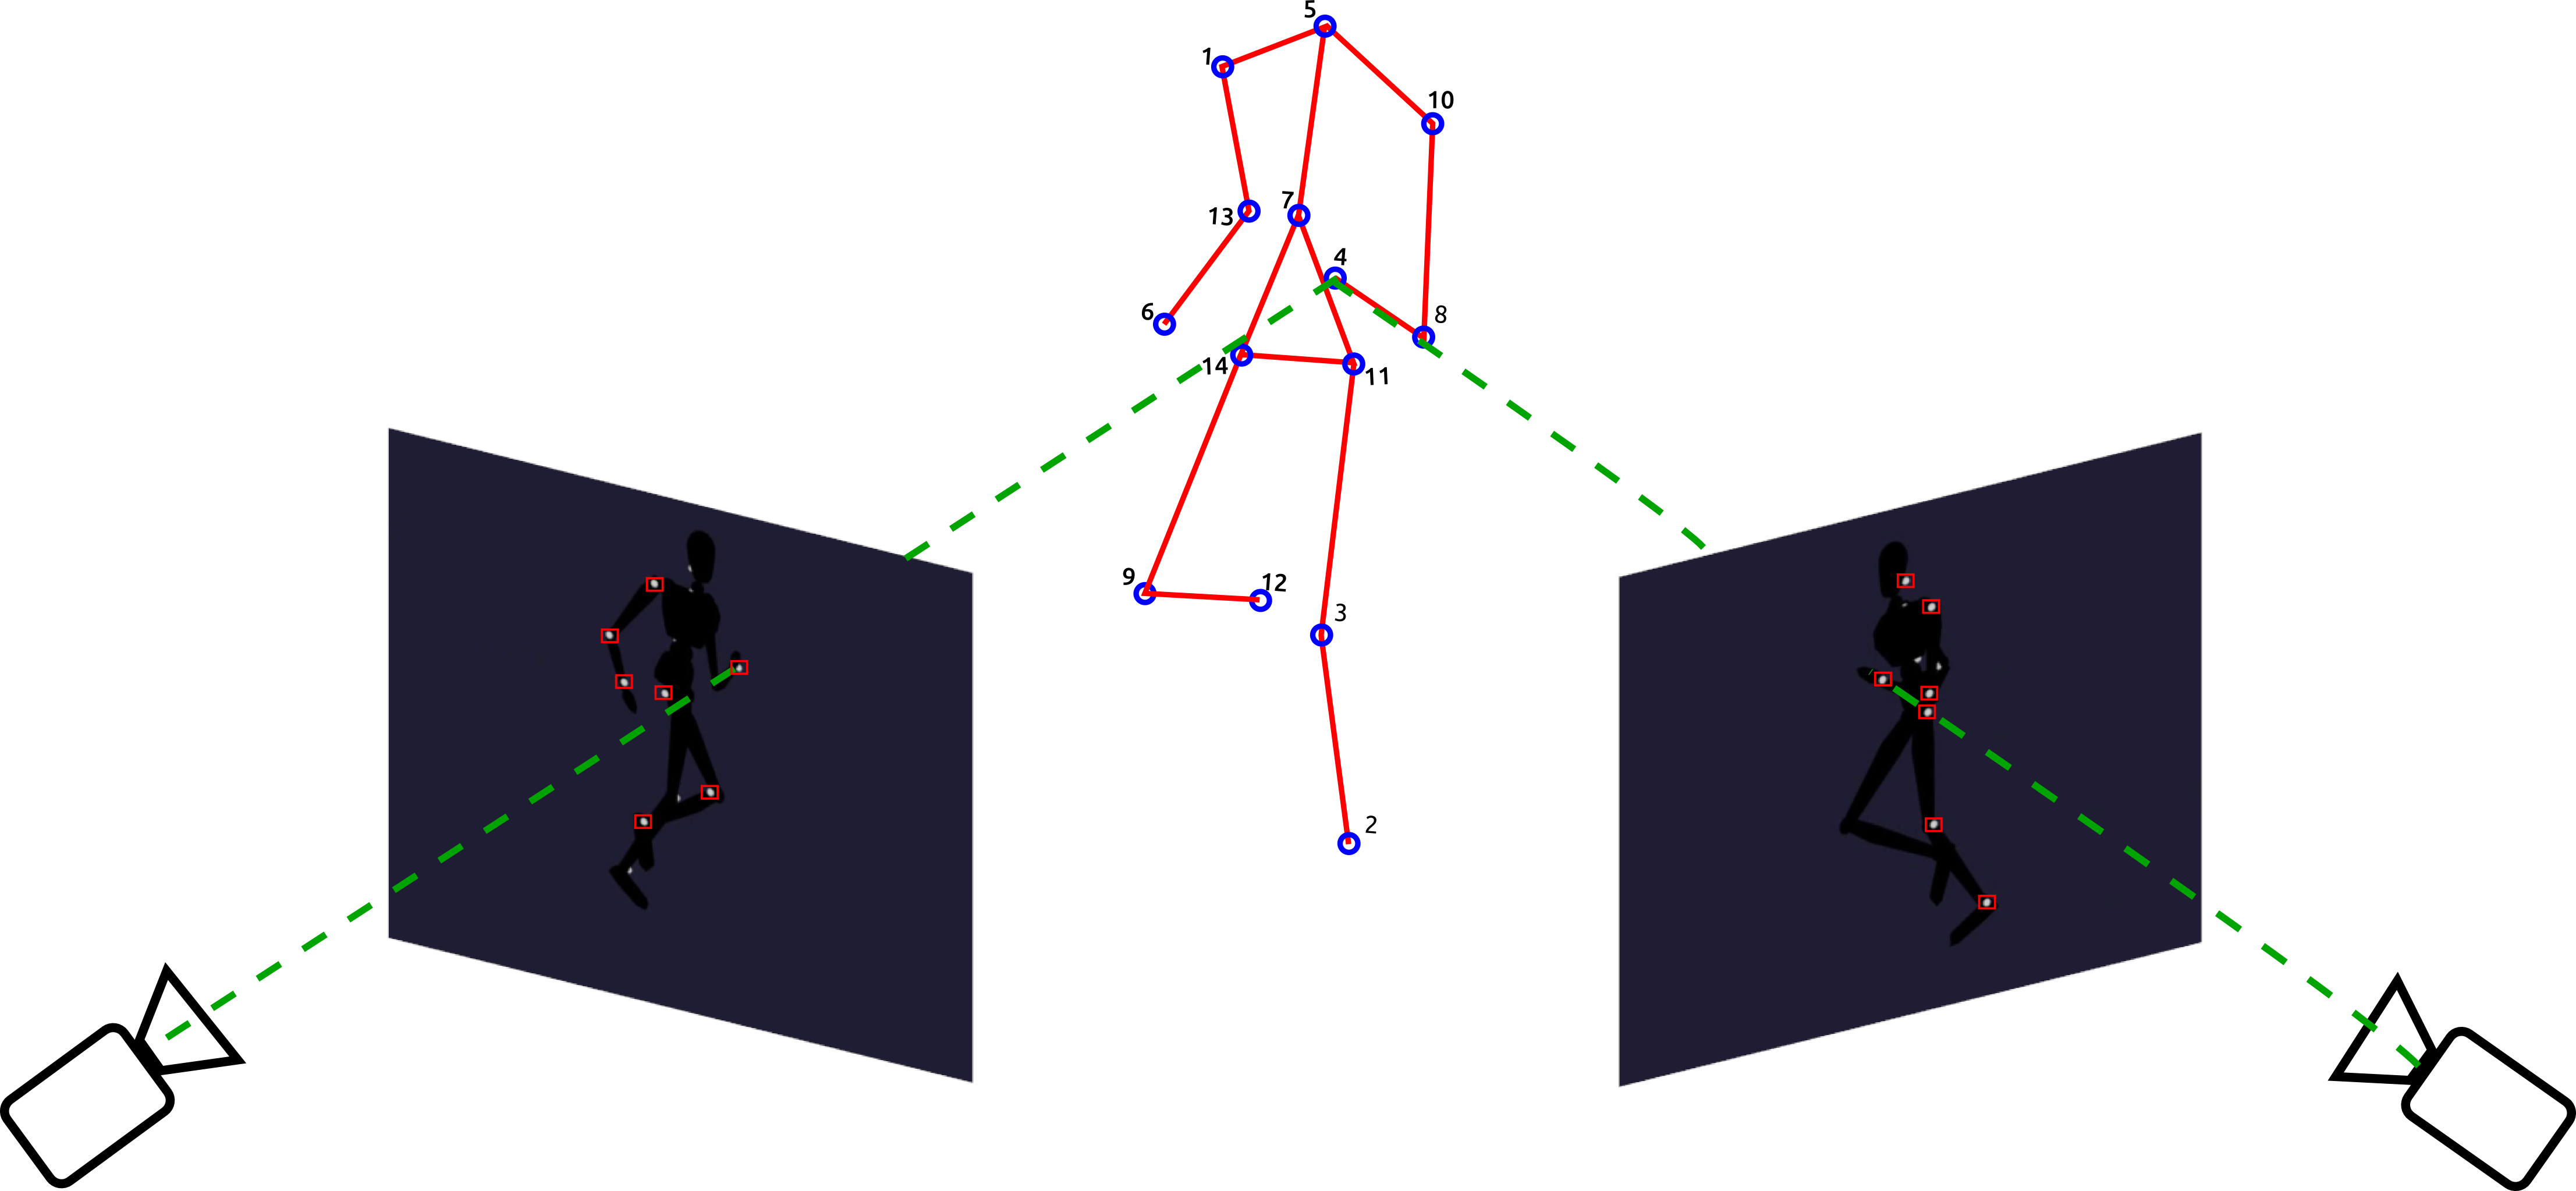
\includegraphics[scale=0.20]{img/Reconstruccion/ejemplo_reconstruccion.png}
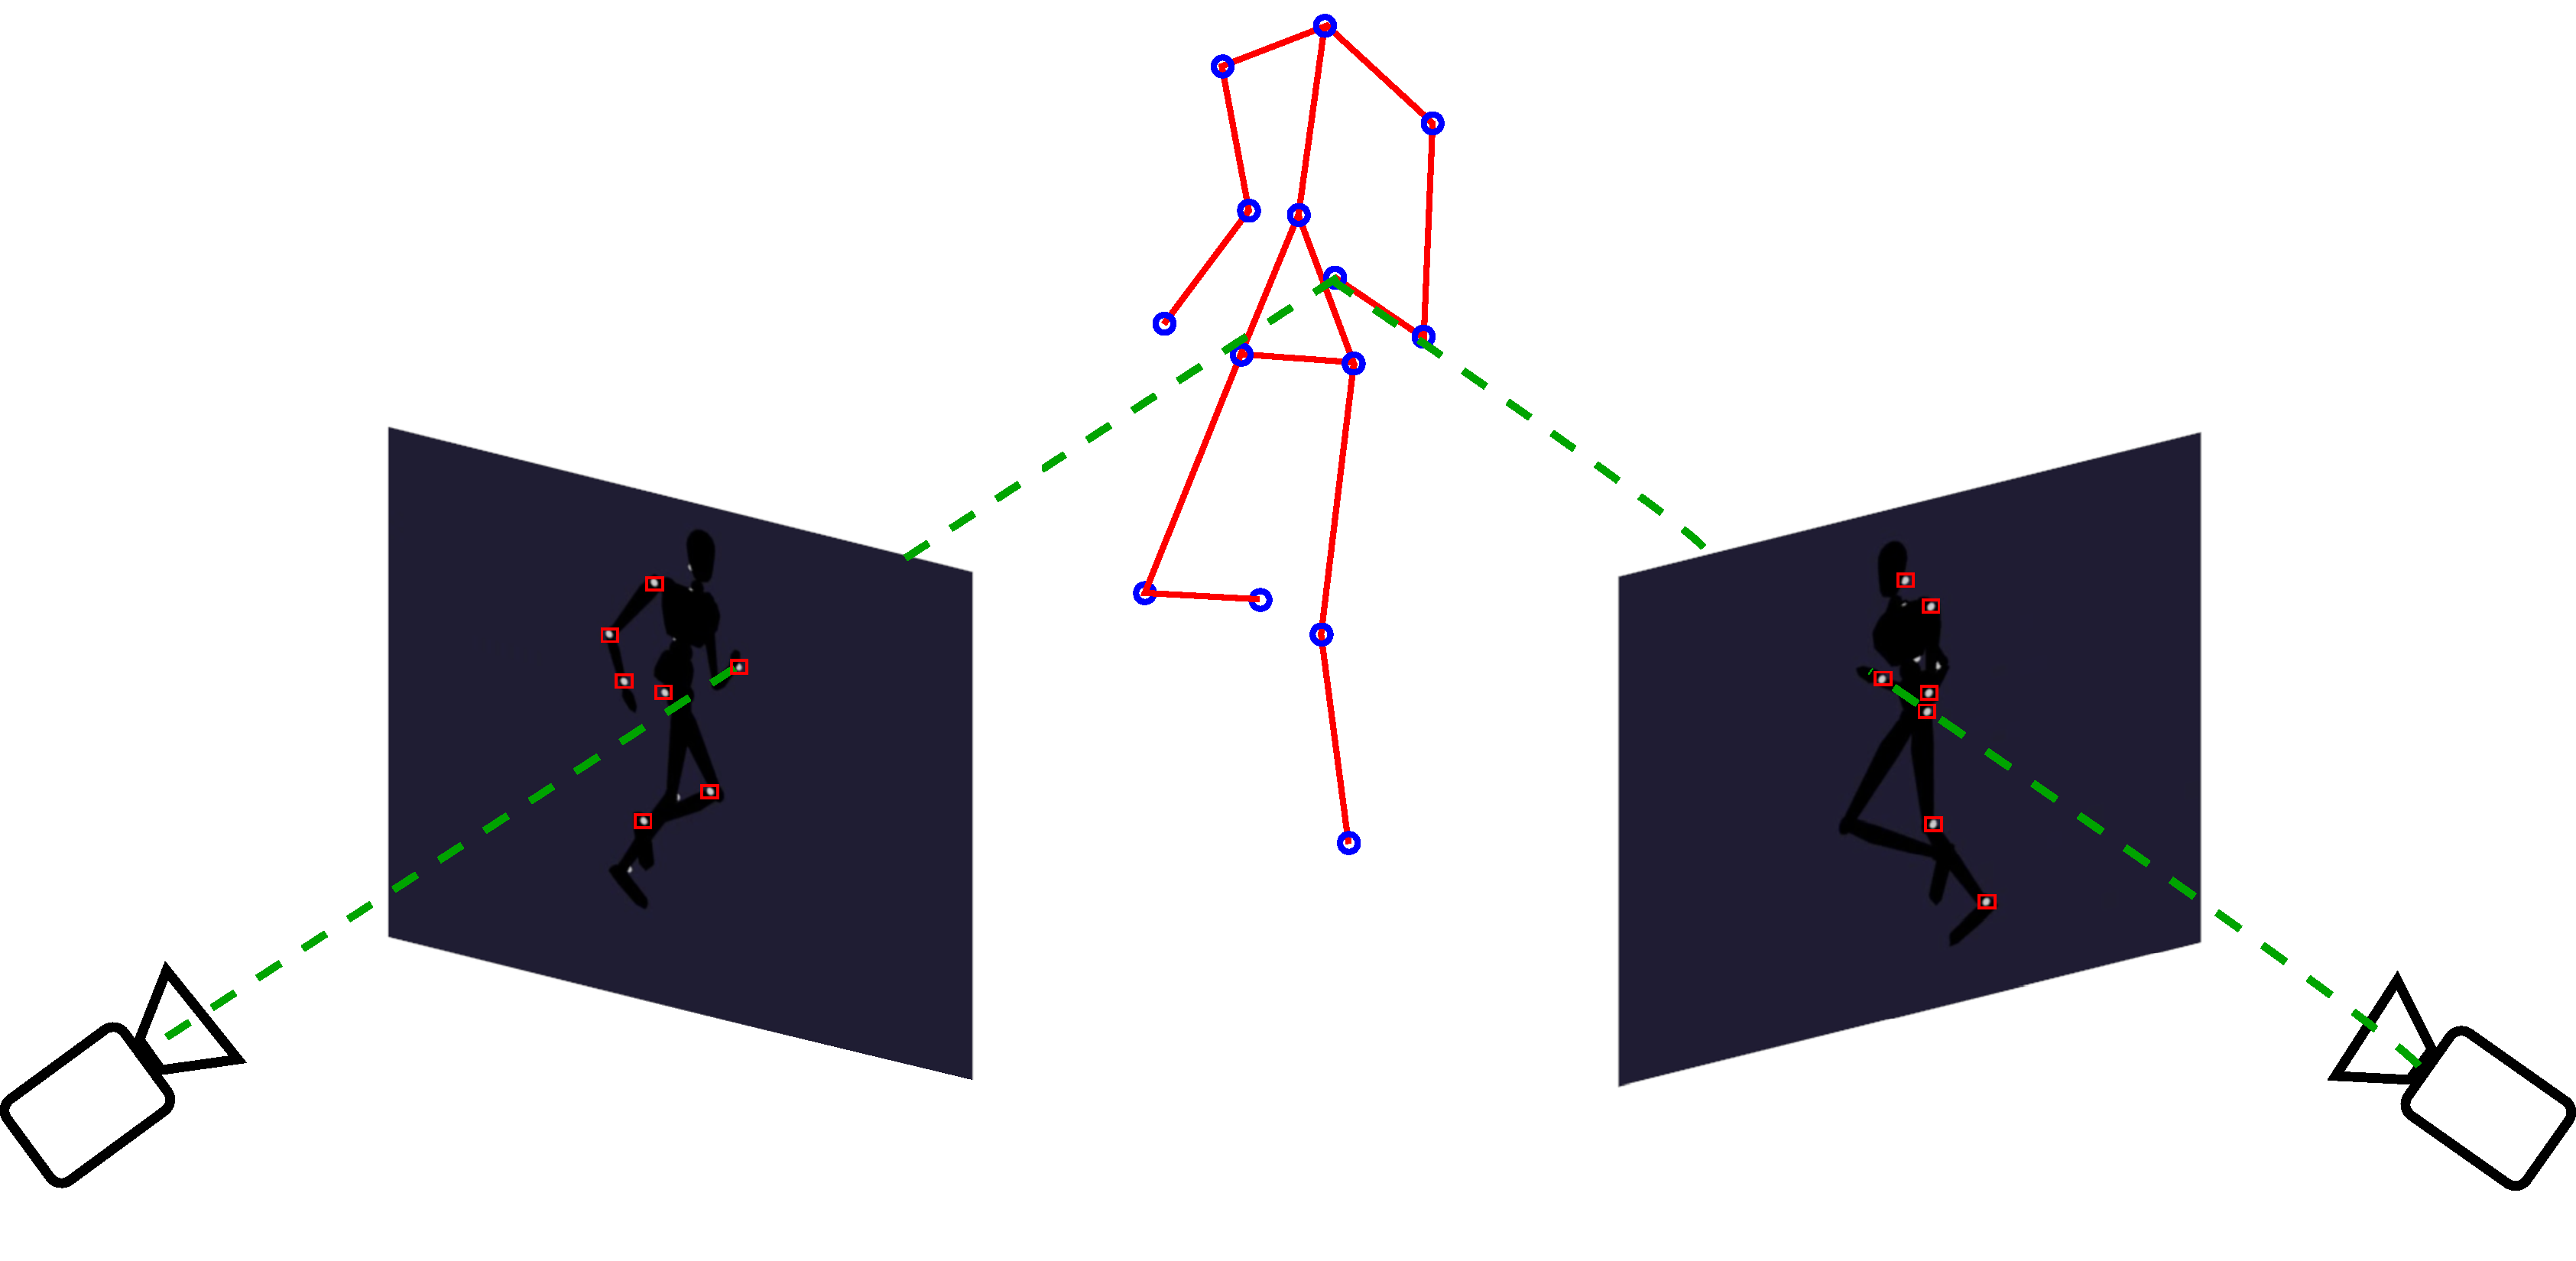
\includegraphics[scale=0.20]{img/Reconstruccion/reconstruccion}
\end{center}
\caption{Reconstrucción con dos cámaras.}
\label{fig: esquema_reconstruccion}
\end{figure}

%Se observa en la figura a uno de los marcadores detectados desde las dos vistas y su correspondiente punto 3D reconstruido.\\
El proceso de reconstrucción implementado fue inspirado en el trabajo de Herda \cite{herda} y consiste en tres pasos fundamentales:
\begin{enumerate}
\item Determinar aquellos marcadores detectados en las distintas cámaras que corresponden a un mismo marcador en el espacio. De esta manera se establece una correspondencia entre los marcadores detectados en las distintas vistas. Dichas asociaciones se establecen de a pares de cámaras.
\item Una vez establecidas estas correspondencias se selecciona aquella que bajo algún criterio, pueda considerarse con mayores posibilidades de ser una asociación correcta. Luego se determina la posición en el espacio del marcador a partir de la asociación seleccionada.
\item Una vez reconstruido uno de los marcadores debe verificarse si dicho marcador fue detectado en el resto de las cámaras.
\end{enumerate}


\section{Geometría epipolar}



Para explicar el algoritmo de reconstrucción es necesario describir brevemente algunos conceptos fundamentales de la geometría epipolar.  Dicha geometría es la que se presenta cuando dos cámaras en distintas posiciones se encuentran capturando el mismo espacio 3D. El análisis de esta situación permite obtener relaciones entre los puntos 3D con sus correspondientes proyecciones en las cámaras, así como las relaciones entre los propios puntos proyectados en las distintas cámaras\cite{cyganek}\cite{hartley}. \\


 Como se muestra en la Figura \ref{fig: geometria_epipolar}, se tiene el caso en que dos cámaras observan un mismo punto 3D en el espacio, el punto $X$. Para esto se considera el modelo \textit{pinhole} de la cámara  descrito en el Capítulo \ref{calibracion}. En ese caso los puntos $O_1$ y $O_2$ son los centros o focos de las cámaras.\\
 
 \begin{figure}[ht!]
 \begin{center}
 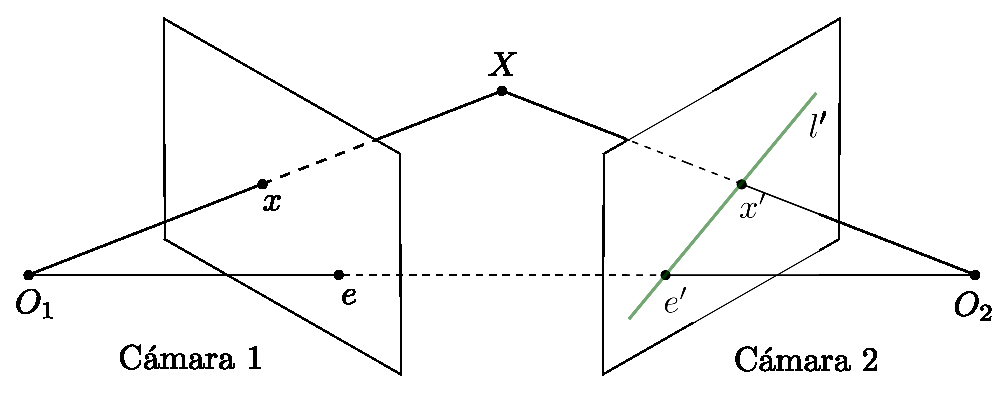
\includegraphics[scale=0.7]{img/Reconstruccion/geometria_epipolar}
 \end{center}
 \caption{Geometría epipolar.}
 \label{fig: geometria_epipolar}
 \end{figure}
 
  El punto $X$ se proyecta en dichas cámaras en los puntos $x$ y $x'$. Es decir, $x$ pertenece a la intersección de la retina de la cámara 1, con el rayo de proyección $\overline{O_1X}$. Análogamente el punto $x'$ pertenece a la intersección de la retina de la cámara 2 con el rayo de proyección $\overline{O_2X}$. A su vez, los focos de ambas cámaras $O_1$ y $O_2$ definen un rayo que corta a las retinas de las cámaras en los puntos $e$ y $e'$ llamados epipolos.\\
  
  Si el punto $X$ varía sobre el espacio 3D, se tienen múltiples rayos de proyección que pasan por dicho punto y el foco de la cámara 1, el punto $O_1$. Dado que $O_1$ se proyecta en la cámara 2 como el punto $e'$ en el plano imagen, todas los rayos  $\overline{O_1X}$ se proyectan en dicha cámara como rectas que se intersecan en el punto $e'$, a estas rectas se les denomina rectas epipolares. Análogamente los sucesivos rayos de proyección $\overline{O_2X}$ se proyectan sobre la cámara 1 como rectas epipolares que se intersecan en el punto $e$. De esta manera se tiene que los puntos $X$, $O_1$ y $O_2$ forman un plano, llamado plano epipolar,  que interseca a los planos imagen en las rectas epipolares.\\
  
De lo anterior se observa que teniendo la proyección $x$ de un punto $X$ sobre la cámara 1, también se conoce la recta epipolar $l'$ y se puede ver que el punto $X$ se proyecta en la cámara 2 en un punto $x'$ situado en dicha recta epipolar $l'=\overline{e'x'}$. Esto implica que por cada punto visto en una retina en la otra se observa una línea.\\
 
Si los puntos $x$ y $x'$ son conocidos, sus rayos de proyección son también conocidos y si estos puntos corresponden a un mismo punto 3D sus rayos de proyección deben interceptarse en $X$. Por lo tanto las coordenadas del punto X pueden derivarse a partir de las coordenadas de sus puntos imagen.\\
 
Para el caso de cámaras reales se tienen distorsiones de ruido, imperfecciones en las lentes de las cámaras, etc. que producen que las proyecciones sean tal que el punto 3D, su proyección en la cámara y el foco de la misma no sean colineales, por lo tanto la proyección real de un punto 3D va a ser aproximadamente el punto ideal de su proyección. \\

\subsection{Matriz Fundamental}

La matriz fundamental es la representación algebraica de la geometría epipolar. Si se tiene el punto $X$ y sus correspondientes proyecciones $x$ y $x'$ en las cámaras, se verifica la siguiente condición :

\begin{equation}
(x')^T F x = 0
\label{ec: matriz fundamental}
\end{equation}
siendo  $F$ la matriz fundamental y $x$, $x'$ las proyecciones en coordenadas homogéneas.\\

Supongamos que se tienen para la cámara 1, la matriz de proyección $P$ y el punto $x$ mencionado anteriormente. El rayo de proyección $\overline{O_1X}$  puede describirse en forma paramétrica como:

\begin{equation}
	X(\lambda) = P^+x+\lambda O_1
\end{equation}

\hspace{-0.6cm}donde $P^+$ es la pseudo-inversa de $P$, tal que $PP^+=I$.\
En particular se toman dos puntos de esa recta, el punto $P^+x$ ($\lambda = 0$) y el punto $O_1$ ($\lambda = \infty$).\
Si se proyectan estos puntos en la cámara 2 se obtienen los puntos $P'P^+x$ y $P'O_1$ respectivamente, siendo $P'$ la matriz de proyección de la cámara 2. Estos puntos pertenecen a la recta epipolar:

\begin{equation}
l' = (P'O_1) \times (P'P^+ x)
\end{equation}

El punto $P'O_1$ es el epipolo $e'$ de la cámara 2. Por lo tanto se tiene que\\$l' = e' \times (P'P^+) x$, donde se define la matriz fundamental como:

\begin{equation}
F=e' \times P'P^+
\end{equation}

Si los puntos imagen se corresponden $x \leftrightarrow x'$, entonces $x'$ se encuentra en la recta epipolar $l'=Fx$ correspondiente al punto $x$, lo cual implica que se cumple $0=(x')^Tl'$ y por lo tanto se verifica la condición de la Ecuación \ref{ec: matriz fundamental}. 

Como se explica anteriormente las igualdades de las ecuaciones mostradas se cumplen en condiciones ideales pero no para cámaras reales en las que aparecen los efectos del ruido, etc., por lo tanto cabe esperar que si se tiene un punto $x$ y su correspondiente $x'$, la Ecuación \ref{ec: matriz fundamental} no se verifique exactamente, aunque si debe devolver un valor próximo a cero.\\

Una propiedad básica de esta matriz es que si $F$ es la matriz fundamental del par de cámaras con matrices de proyección ($P,P'$), entonces $F^T$ es la matriz fundamental del par de cámaras en sentido opuesto: ($P',P$). Por otra parte si se tiene el punto $x$ en la imagen de una cámara, su recta epipolar correspondiente en otra cámara es $l'=Fx$. Análogamente $l=F^Tx'$ representa la línea epipolar asociada con $x'$ en la segunda cámara.

\section{Algoritmo propuesto por Herda }

Como se explica en el Capítulo \ref{sec:implementacion_bloques_sistema}, se inicia la implementación de este bloque a partir del algoritmo propuesto por Herda \cite{herda}. Este algoritmo en algunos aspectos no es descripto con el detalle suficiente tal que pueda ser replicado fielmente. Por esta razón su implementación se ha elaborado realizando algunos supuestos en los casos donde su interpretación presenta ambigüedades.\\

Por otra parte, el sistema diseñado por Lorna Herda pretende utilizar la información del esqueleto (ver Capítulo \ref{sec:implementacion_bloques_sistema}), como por ejemplo la posición de articulaciones, distancias entre marcadores, etc. Dado que esta etapa del algoritmo no fue implementada resultó necesario robustecer el proceso de reconstrucción en las partes del algoritmo donde no se utiliza esta información.\\


Además, este algoritmo utiliza la triangulación estéreo para reconstruir un punto 3D a partir de los puntos 2D detectados en las distintas vistas. La correspondencia entre distintas vistas se establece mediante la matriz fundamental, cuyos conceptos fueron explicados en la sección anterior. Esta matriz se puede obtener luego del proceso de calibración.\\

Las ideas que sigue el algoritmo se describen a continuación:\

\begin{itemize}
\item Se toman dos vistas y se realiza el test de la condición epipolar (Sección \ref{MejorAsociacion}). Si existe una asociación no ambigua se reconstruyen  las coordenadas 3D a partir de las coordenadas 2D.

\item Las coordenadas 3D reconstruidas se re-proyectan en las cámaras restantes. Los puntos 2D encontrados en esa re-proyección son asociados al punto 3D. De esta forma se tiene por cada punto 3D, sus correspondientes puntos 2D asociados en las distintas vistas.\

\item Se considera que un marcador 3D está correctamente reconstruido si se re-proyecta en al menos una cámara. A este tipo de reconstrucción se le llama \textit{reconstrucción trinocular}.

\item Si el número de marcadores reconstruidos es inferior al número de marcadores colocados sobre la persona, entonces se realiza una segunda asociación entre dos vistas. En este caso la reconstrucción se realiza solamente con dos vistas (\textit{reconstrucción binocular}).\\

\end{itemize}

Posteriormente el algoritmo plantea realizar ciertos chequeos sobre los puntos reconstruidos de manera de validarlos. Dichos chequeos utilizan información del esqueleto (Figura \ref{fig:oclusion_herda}).


Lo que se busca verificar en dichos chequeos, es que para un determinado cuadro los marcadores sean efectivamente visibles por aquellas cámaras que los reconstruyeron y no están ocultos por alguna parte del cuerpo, lo que evidenciaría que la reconstrucción es incorrecta. Si esto llegara a suceder, el algoritmo busca otras vistas de las cuales reconstruir el marcador.

\begin{figure}[ht!]
 \begin{center}
 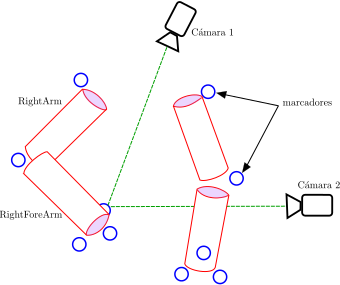
\includegraphics[scale=0.8]{img/Reconstruccion/oclusion_herda}
 \end{center}
 \caption{Chequeo de visibilidad y oclusión \cite{herda}.}
 \label{fig:oclusion_herda}
 \end{figure}


\section{Algoritmo implementado}

En la Sección anterior se describió el algoritmo de reconstrucción propuesto en el sistema de Herda, sin embargo, el algoritmo implementado no es exactamente el mismo. Como se aclara sobre el final de la Sección \ref{sec:implementacion_bloques_sistema} , la cantidad de módulos a implementar es grande, presentando ambigüedades importantes que dificultan en muchos casos su reproducibilidad, considerando los tiempos con los que cuenta el proyecto, se decide dar prioridad a los bloques principales, comenzando por lo básico e implementando módulos hasta lograr la performance necesaria. A continuación se describe la implementación realizada para este proyecto y las diferencias con el algoritmo de reconstrucción propuesto por Herda.\\

El algoritmo implementado recibe como entrada los puntos 2D de los marcadores detectados y devuelve como salida los puntos 3D reconstruidos. El primer paso consiste en establecer una asociación entre ciertos puntos 2D de distintas cámaras. Luego, se pasa a un conjunto de bloques que se ejecutan de manera iterativa hasta que no queden marcadores para reconstruir. En dicho bloque se busca la mejor asociación entre puntos, bajo determinado criterio, luego se reconstruye un punto 3D y se realiza un proceso de validación de dicha reconstrucción. En la iteración siguiente se actualizan las asociaciones que habían sido establecidas previamente. Cuando no hay más marcadores para reconstruir se detiene el proceso iterativo y se devuelven aquellos marcadores que fueron reconstruidos en cada iteración. En la Figura \ref{fig: diagrama algoritmo} se presenta un diagrama del algoritmo.\\

\begin{figure}[ht!]
\hspace{-1cm}
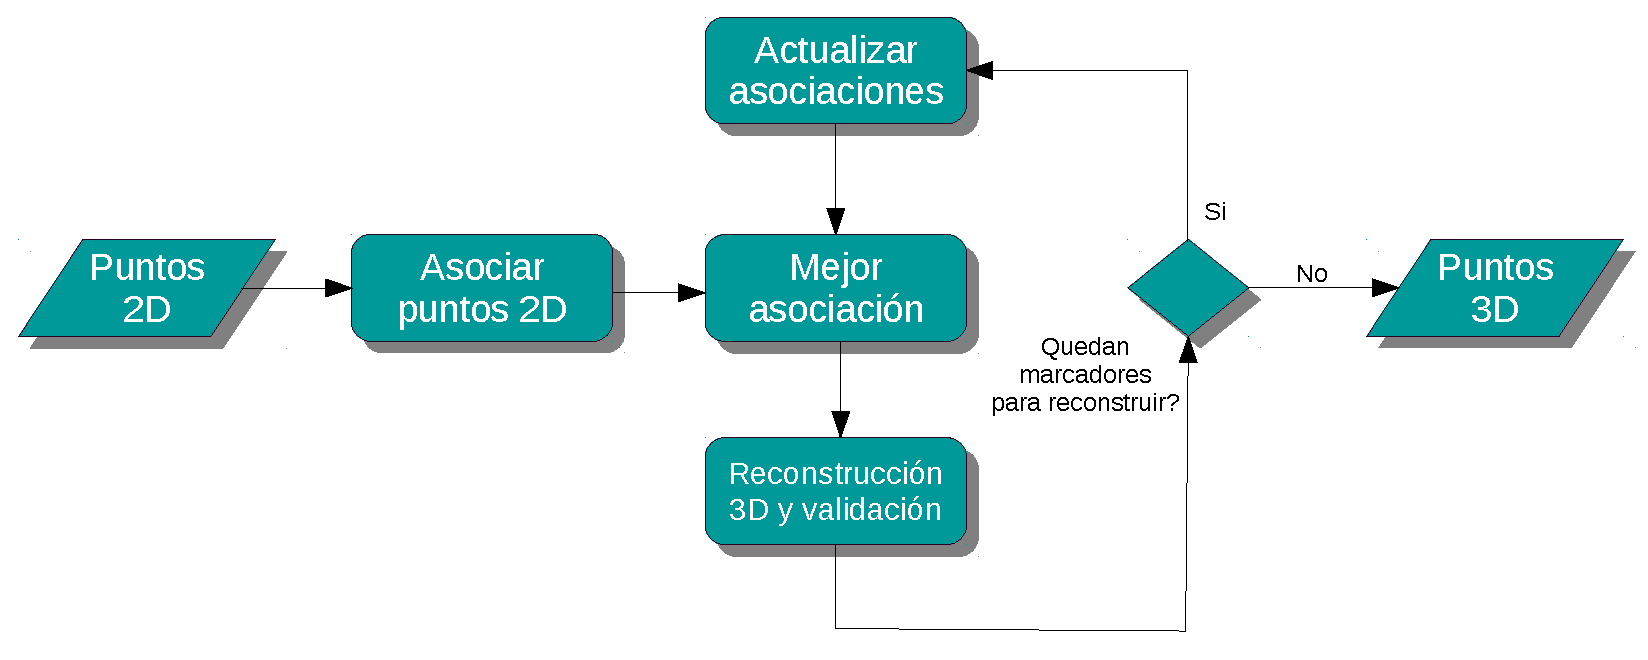
\includegraphics[scale=0.55]{img/Reconstruccion/diagrama_algoritmo.pdf}
\caption{Diagrama del algoritmo implementado.}
\label{fig: diagrama algoritmo}
\end{figure}

A continuación se describe el funcionamiento de cada uno de los bloques.

\subsection{Asociar puntos 2D}\label{seccion_asociar2D_uno}

Este bloque recibe como entrada las coordenadas de los puntos detectados en cada una de las cámaras, parámetros de las mismas tales como sus matrices de proyección y devuelve para cada punto una lista ordenada por relevancia, de las asociaciones existentes con puntos en otras cámaras.
Basándose en lo explicado anteriormente el proceso  se puede ejemplificar  en la Figura \ref{fig: cam2cam }.

\begin{figure}[ht!]
\hspace{0.3cm}
\includegraphics[scale=0.7]{img/Reconstruccion/cam2cam2}
\caption{Asociación de puntos 2D en dos cámaras.}
\label{fig: cam2cam }
\end{figure}

En primer lugar se seleccionan dos cámaras y se considera un punto en una de ellas, por ejemplo el punto $x_{11}$ de la cámara 1, y se evalúa la Ecuación \ref{ec: matriz fundamental} para cada punto en la cámara 2. Esto equivale a proyectar la recta epipolar $l'$ correspondiente al punto $x_{11}$ sobre la cámara 2  y tomar las distancias de los puntos detectados en la cámara 2 a la recta $l'$. Se demuestra que dicha distancia difiere a menos de un factor de escala respecto al valor obtenido al evaluar la Ecuación \ref{ec: matriz fundamental}. Se asume que los puntos de la cámara 2 que tengan mayor posibilidad de corresponder con el punto $x_{11}$, son aquellos que al ser evaluados por la ecuación obtienen valores próximos a cero.
De esta manera se obtiene para cada punto en la cámara 1 un conjunto de puntos en la cámara 2 ordenados según su distancia a la recta epipolar correspondiente.
Repitiendo el procedimiento de manera inversa, esto es, de la cámara 2 a la cámara 1, se obtiene igualmente para cada punto de la cámara 2  los puntos de la cámara 1 ordenados según su proximidad a la recta epipolar correspondiente. A continuación se toman otros pares de cámaras y se vuelve a repetir el proceso. 

Es importante resaltar que para la elección de los pares de cámaras se han considerado dos casos.
El primero de ellos evalúa cada cámara respecto a todas las restantes y el segundo considera la disposición de las cámaras en el espacio y empareja las cámaras adyacentes de manera consecutiva (ver Figura \ref{img_asociacion}). %Más adelante se demuestra que este segundo procedimiento da mejores resultados.ACÁ SE DEBE REFERENCIAR BIEN DONDE ESTA ESA DEMOSTRACIÓN \\

 \begin{figure}[ht!]
   \centering 
    \subfloat[Cada cámara con las restantes. Ejemplo de emparejamiento de la cámara 1.]{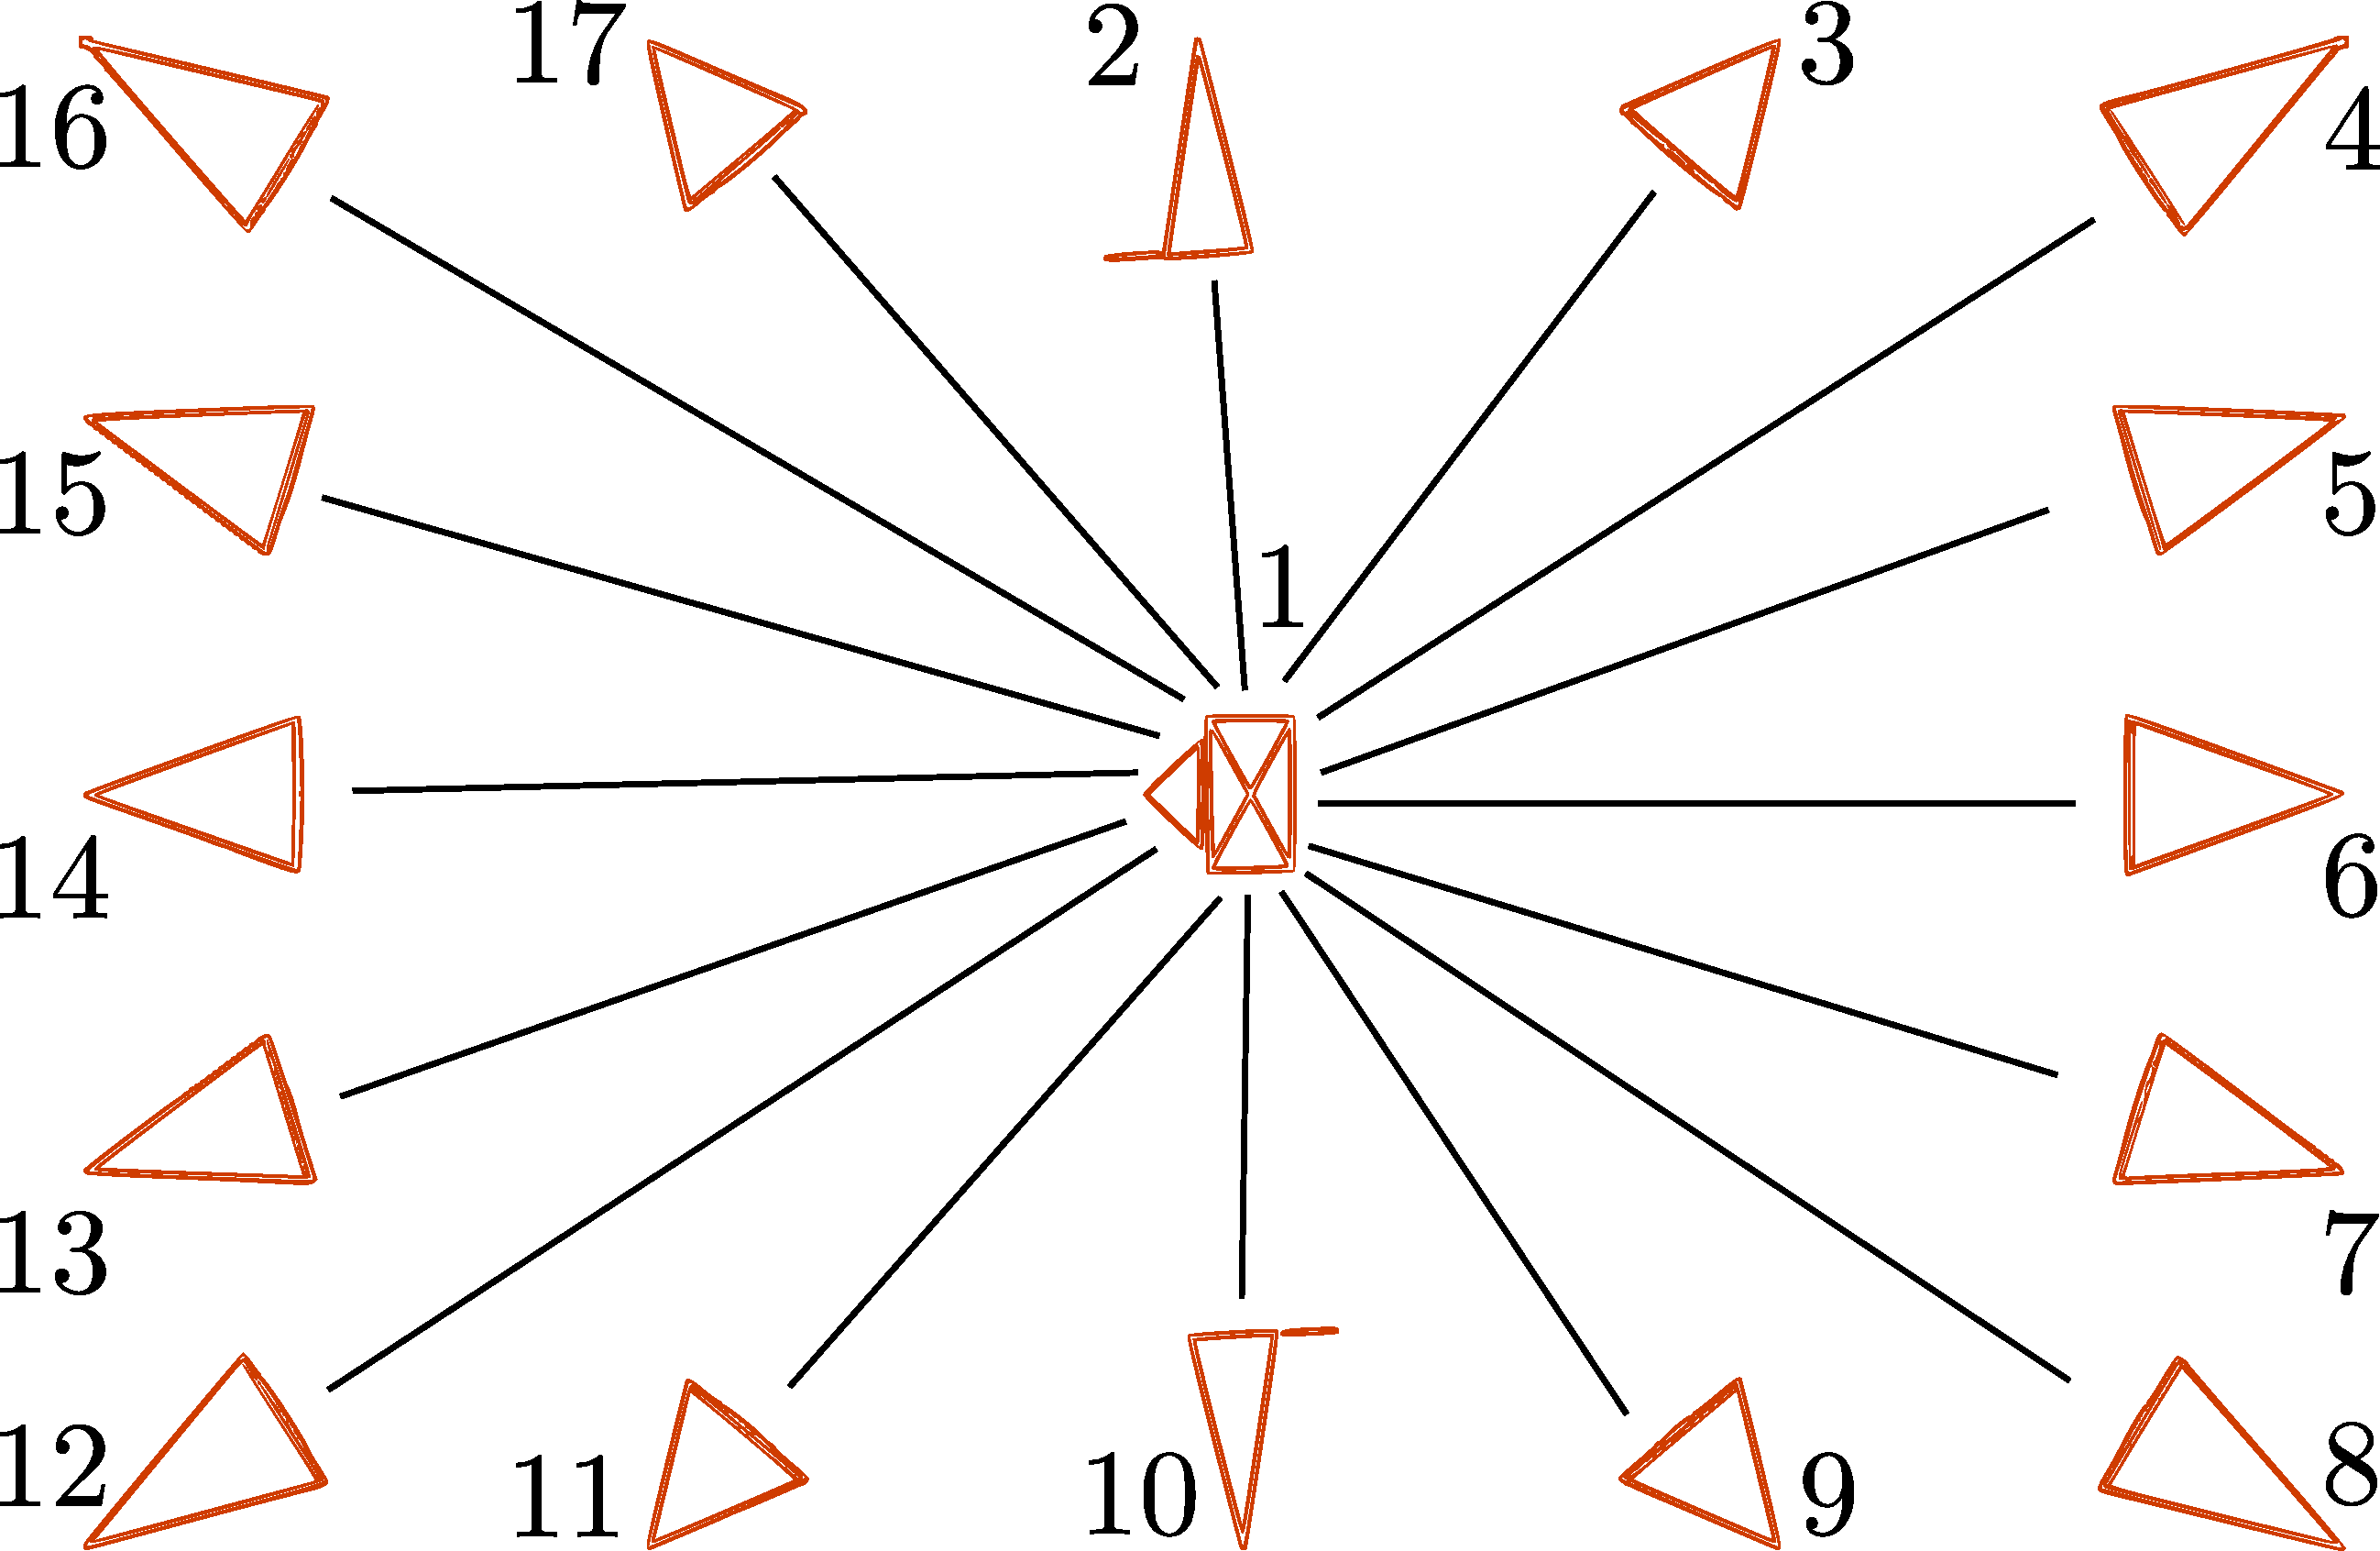
\includegraphics[scale=0.13]{img/Reconstruccion/enlazado_general}}\hspace{2cm}
    \subfloat[Cada cámara con su adyacente]{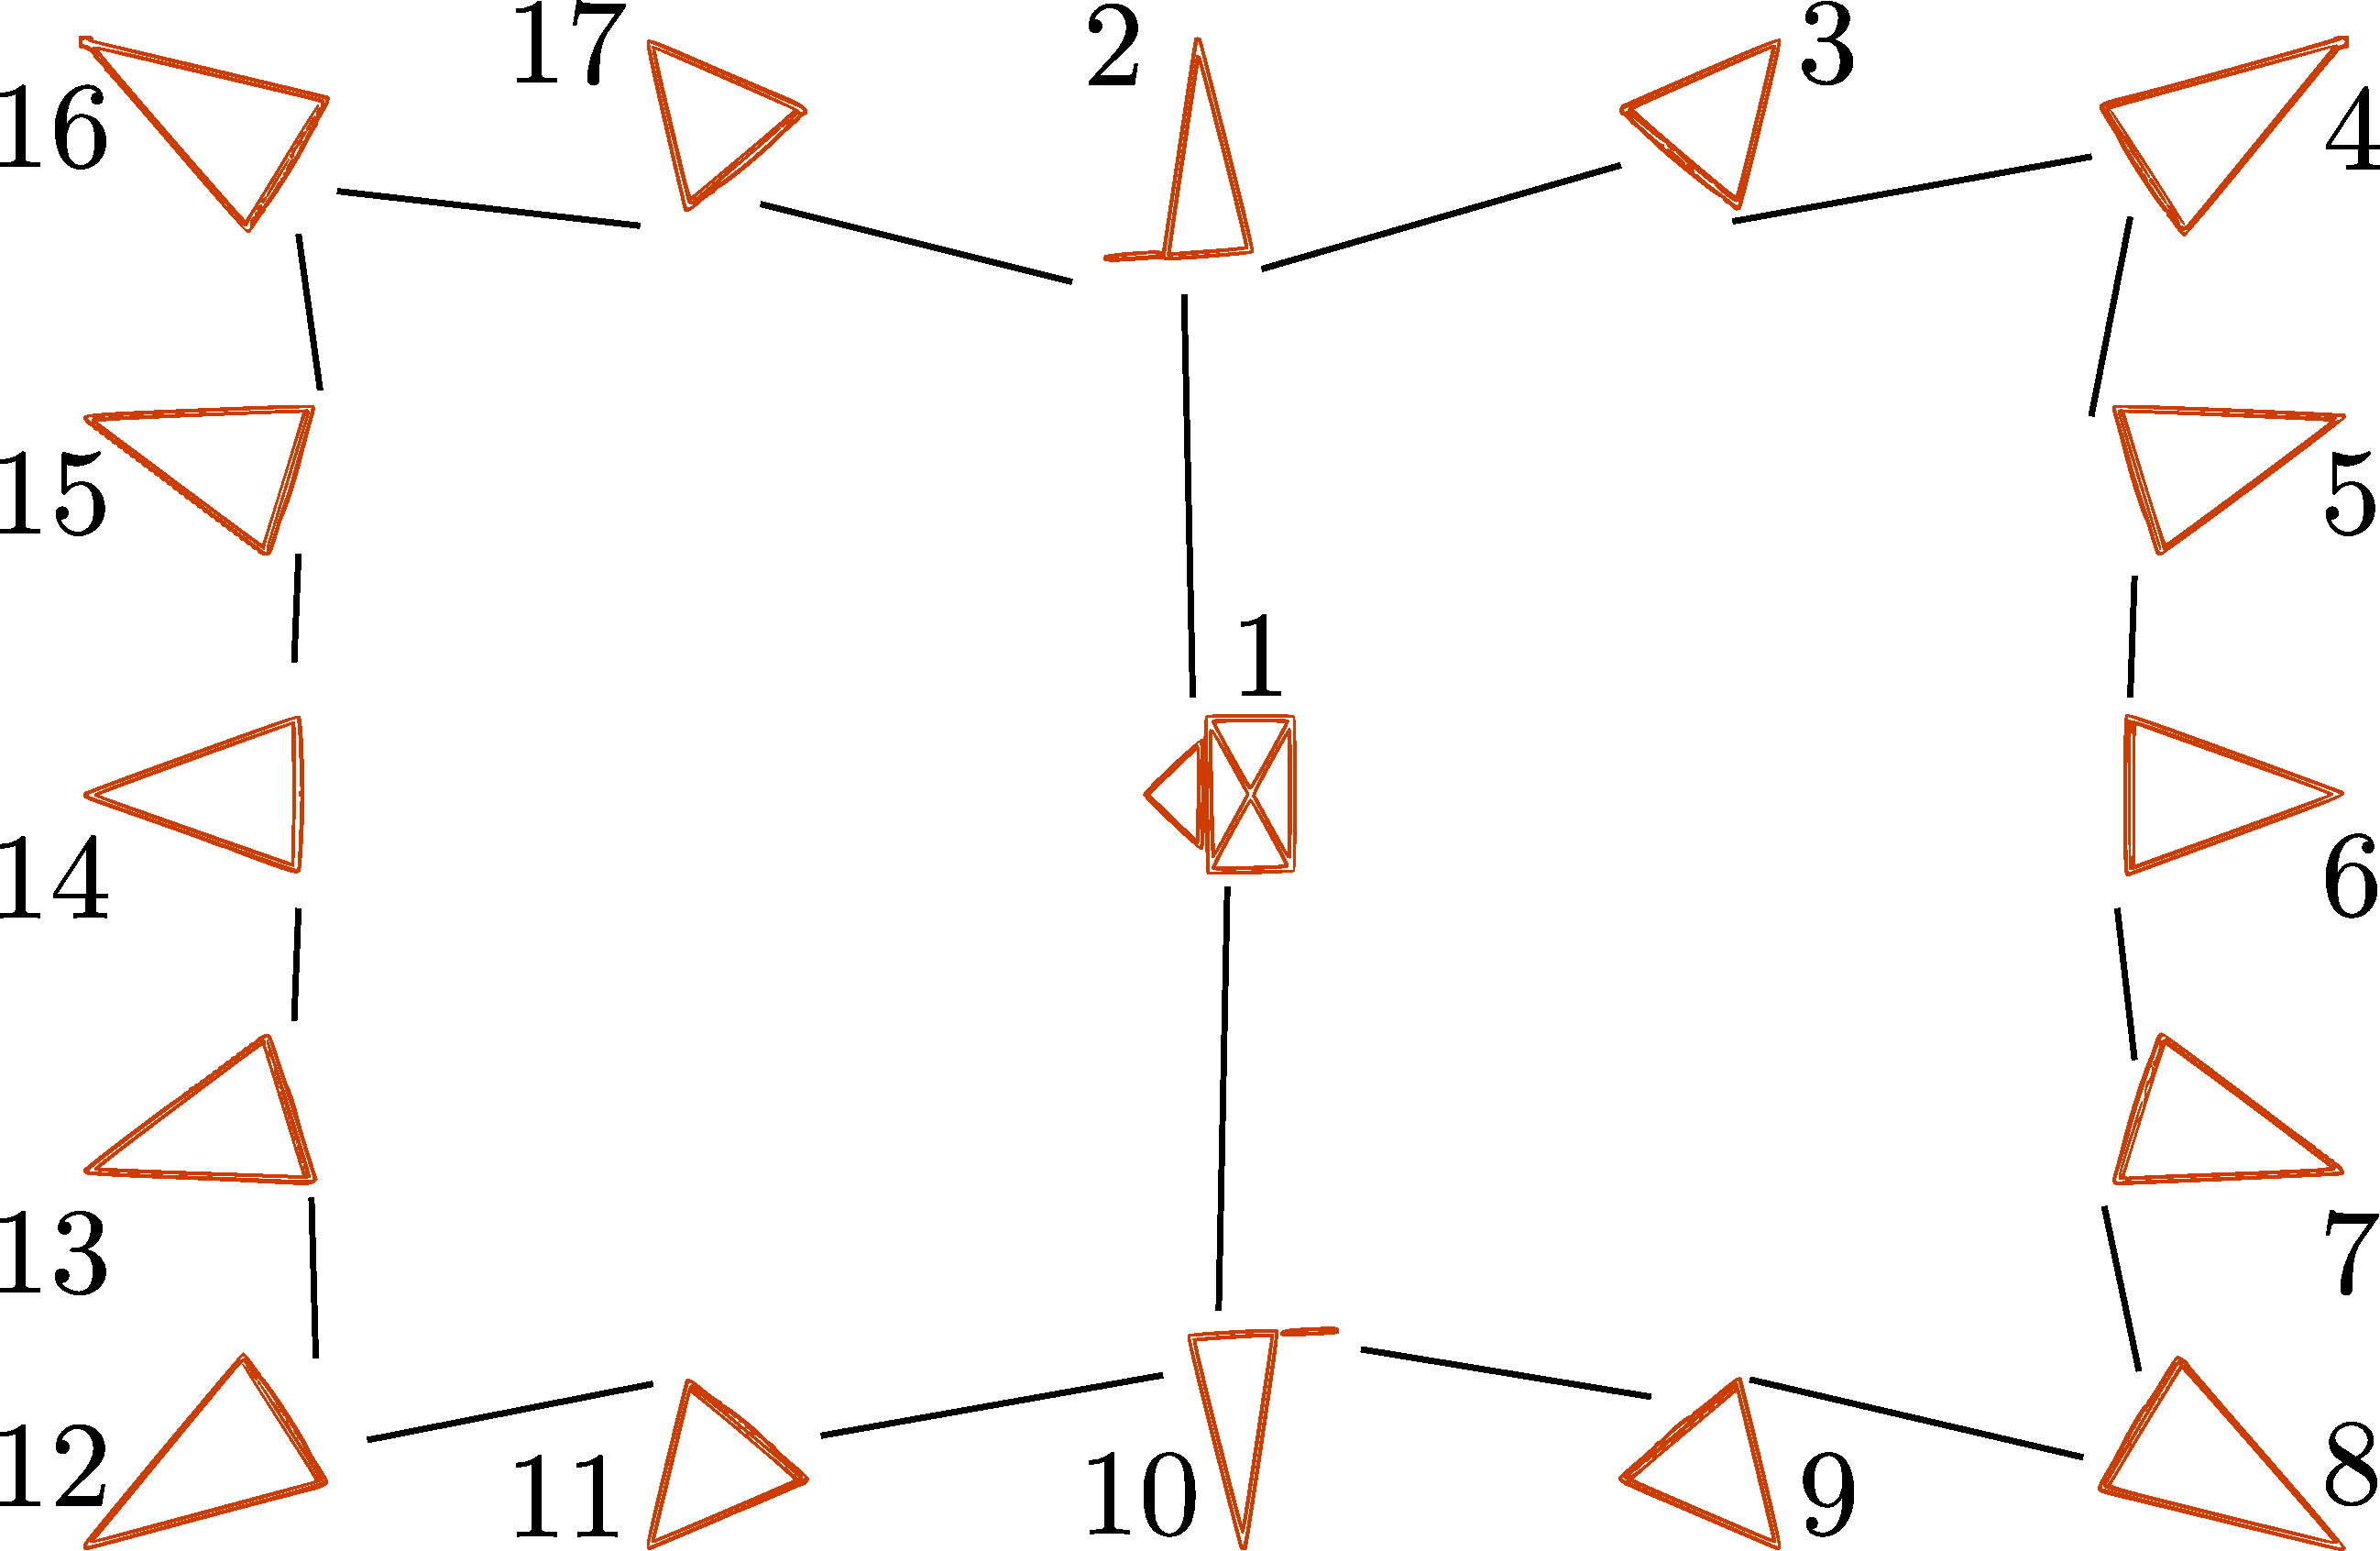
\includegraphics[scale=0.13]{img/Reconstruccion/enlazado_adyacente}\label{img_asociacion_consecutivas}}
   \caption{Métodos utilizados para generar pares de cámaras.}  
   \label{img_asociacion} 
 \end{figure} 





\subsection{Mejor asociación}\label{MejorAsociacion}

A partir de la lista con asociaciones entre puntos de dos vistas generada anteriormente, es necesario elegir aquella que posea mayor probabilidad de conformar la pareja de imágenes correspondiente a la proyección de un marcador 3D sobre dichas vistas.
%corresponder a la proyección en esas dos vistas de uno de los marcadores en el espacio.\\


Recordando que todas las asociaciones de puntos entre pares de cámaras se encuentran ordenadas por distancia, se toma aquella asociación que posea la menor distancia y contenga puntos válidos, descartando las restantes. Un punto se considera válido si en iteraciones anteriores no se a podido asociar a ningún punto 3D reconstruido (ver Sección \ref{actualizar_asociaciones}).
De esta forma cada punto de una cámara es asociado, si existen puntos válidos, con un punto en otra de las cámaras.


 Supongamos en la Figura \ref{fig: geometria_epipolar} que los puntos $x$ y $x'$ son la mejor asociación entre la cámara 1 y la cámara 2, y efectivamente son imágenes de un mismo punto 3D, idealmente los rayos de proyección se interceptarían en $X$, pero debido a incertidumbres en los procesos de calibración y segmentación la distancia entre dichos rayos no es nula, en el mejor de los casos solo es próxima a cero. 
Para evaluar cuál es entre los pares de puntos asociados disponibles el par que posee mayor posibilidad de corresponder a las proyecciones de un punto 3D, se proyectan todos los rayos de proyección y se toma aquella pareja de puntos que genere rayos de proyección con la menor distancia entre sí.


\subsection{Reconstrucción 3D y validación}\label{seccion_reconstruccion3D_validacion}


Luego de encontrar las mejores asociaciones entre dos cámaras se procede a reconstruirlas. Estas reconstrucciones deben ser validadas, para ello en principio se utiliza el  criterio propuesto por Herda \cite{herda}: se considera que una reconstrucción proveniente de dos cámaras es válida, si al proyectar sobre una tercera cámara existe al menos un punto de esta última que diste menos de un cierto valor umbral. Si efectivamente se encuentra al menos un punto, se asocia con los dos puntos que generaron la reconstrucción y se repite el proceso con el resto de las cámaras. Una vez finalizada la iteración, se retira a la pareja que genera la reconstrucción así como también a los puntos que lograron validarla, y se itera nuevamente repitiendo el proceso con la siguiente mejor pareja asociada entre dos cámaras. \\ 



\begin{figure}[ht!]
\centering
\hspace{-1cm}
\captionsetup{justification=centering,margin=1.0cm}
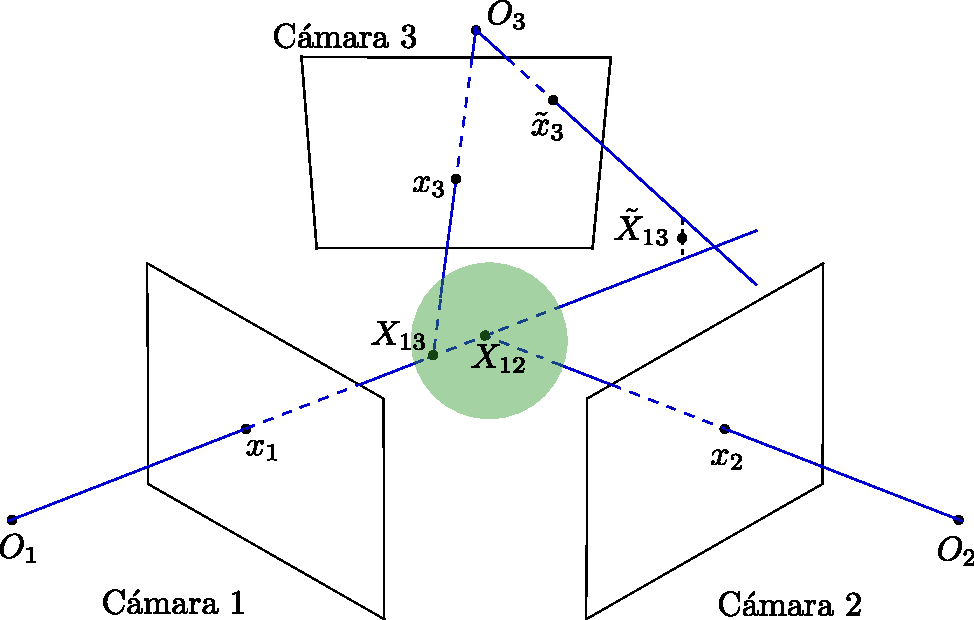
\includegraphics[scale=0.7]{img/Reconstruccion/validacion.pdf}
\caption{Reconstrucción entre cámaras 1, 2 y validación con cámara 3. El punto $x_3$ de la cámara 3 valida la reconstrucción, no así el punto $\tilde{x}_3$.}
\label{img_reconstruccion_validacion}
\end{figure}


El algoritmo desarrollado, si bien conceptualmente es similar, se implementa desde una óptica diferente computacionalmente más eficiente.
En lugar de llevar en cada iteración la información 3D a cada cámara, se procede a llevar la información de las cámaras una sola vez al espacio 3D y trabajar en cada iteración sobre el mismo. 


La información que contiene un punto en una retina se mapea en el espacio 3D sobre el rayo de proyección que contiene a dicho punto y al centro de la cámara correspondiente. Supongamos que se tienen los rayos de proyección en el espacio 3D de todos los puntos contenidos en las retinas y que $x_1$ es un punto en la cámara 1 de centro $O_1$ y $x_2$ es un punto en la cámara 2 de centro $O_2$ se encuentran asociados y reconstruyen al punto $X_{12}$ (ver Figura \ref{img_reconstruccion_validacion}). 


Idealmente $X_{12}$ se genera al interceptar los rayos de proyección de los puntos $x_1$ y $x_2$, pero debido a incertidumbres en la detección de marcadores o la calibración, comúnmente los rayos se van a cruzar. La reconstrucción, se estima como el punto del espacio de menor distancia a ambos rayos, por lo que
$X_{12}$ se encuentra en el punto medio del segmento perpendicular a ambos rayos.



El algoritmo implementado asume que un punto en una cámara, valida a $X_{12}$ si junto a $x_1$ reconstruye un punto 3D que se encuentra dentro de la esfera $B(X_{12}, \delta)$ de centro $X_{12}$ y radio $\delta$, donde $\delta$ es un cierto valor umbral. Notar que la elección anterior de $x_1$ sobre $x_2$ es indiferente para los propósitos de este proyecto. 


Si bien este criterio difiere del postulado original propuesto por Herda, en cierta manera se considera más robusto, pues en el postulado original basta con que dos puntos en una retina se encuentren lo suficientemente cerca para obtener una validación, pero esto no implica necesariamente que provengan de puntos 3D cercanos, sin embargo bajo el nuevo criterio si dos puntos 3D se encuentran cerca, entonces es válido afirmar que sus proyecciones sobre las distintas retinas también deben estarlo. Otra ventaja es que los umbrales bajo los cuales se considera que dos puntos están ``cerca'' difieren en cada una de las cámaras debido al distinto mapeo de distancias, sin embargo en el espacio 3D, manejar un único umbral resulta suficiente.       

\subsection{Actualizar asociaciones}\label{actualizar_asociaciones}

Del bloque anterior se tiene, un punto $X$ reconstruido y sus correspondientes proyecciones en cada una de las cámaras. Dichas proyecciones no deben ser consideradas nuevamente, por tanto estos puntos 2D que reconstruyen $X$, no se consideran como puntos válidos en las siguientes iteraciones.\\



Finalmente el proceso iterativo se detiene cuando no hay más marcadores para reconstruir, lo cual implica que se cumple alguna de las siguientes condiciones:\\
\begin{itemize}
\item el número de marcadores reconstruidos es igual al número de marcadores que tiene colocada la persona, o igual al número máximo de marcadores  reconstruidos que se haya indicado.

\item No existen puntos 2D válidos tal que pueda establecerse una asociación entre puntos de distintas vistas.
\end{itemize}




\section{Resultados de reconstrucción sobre secuencias sintéticas}

Se ha probado el algoritmo descrito anteriormente con secuencias capturadas en Blender. Para la configuración de 17 cámaras se han obtenido resultados aceptables,  con errores promedio en torno a los $0.5\,cm$. En la Sección \ref{seccion_performance}, se define la medida de error  y se evalúa el desempeño del algoritmo respecto a dicha medida. En dichas pruebas se observan resultados aceptables aún utilizando hasta 6 cámaras.

\begin{figure}[ht!]
\centering
\captionsetup{justification=centering,margin=0.2cm}
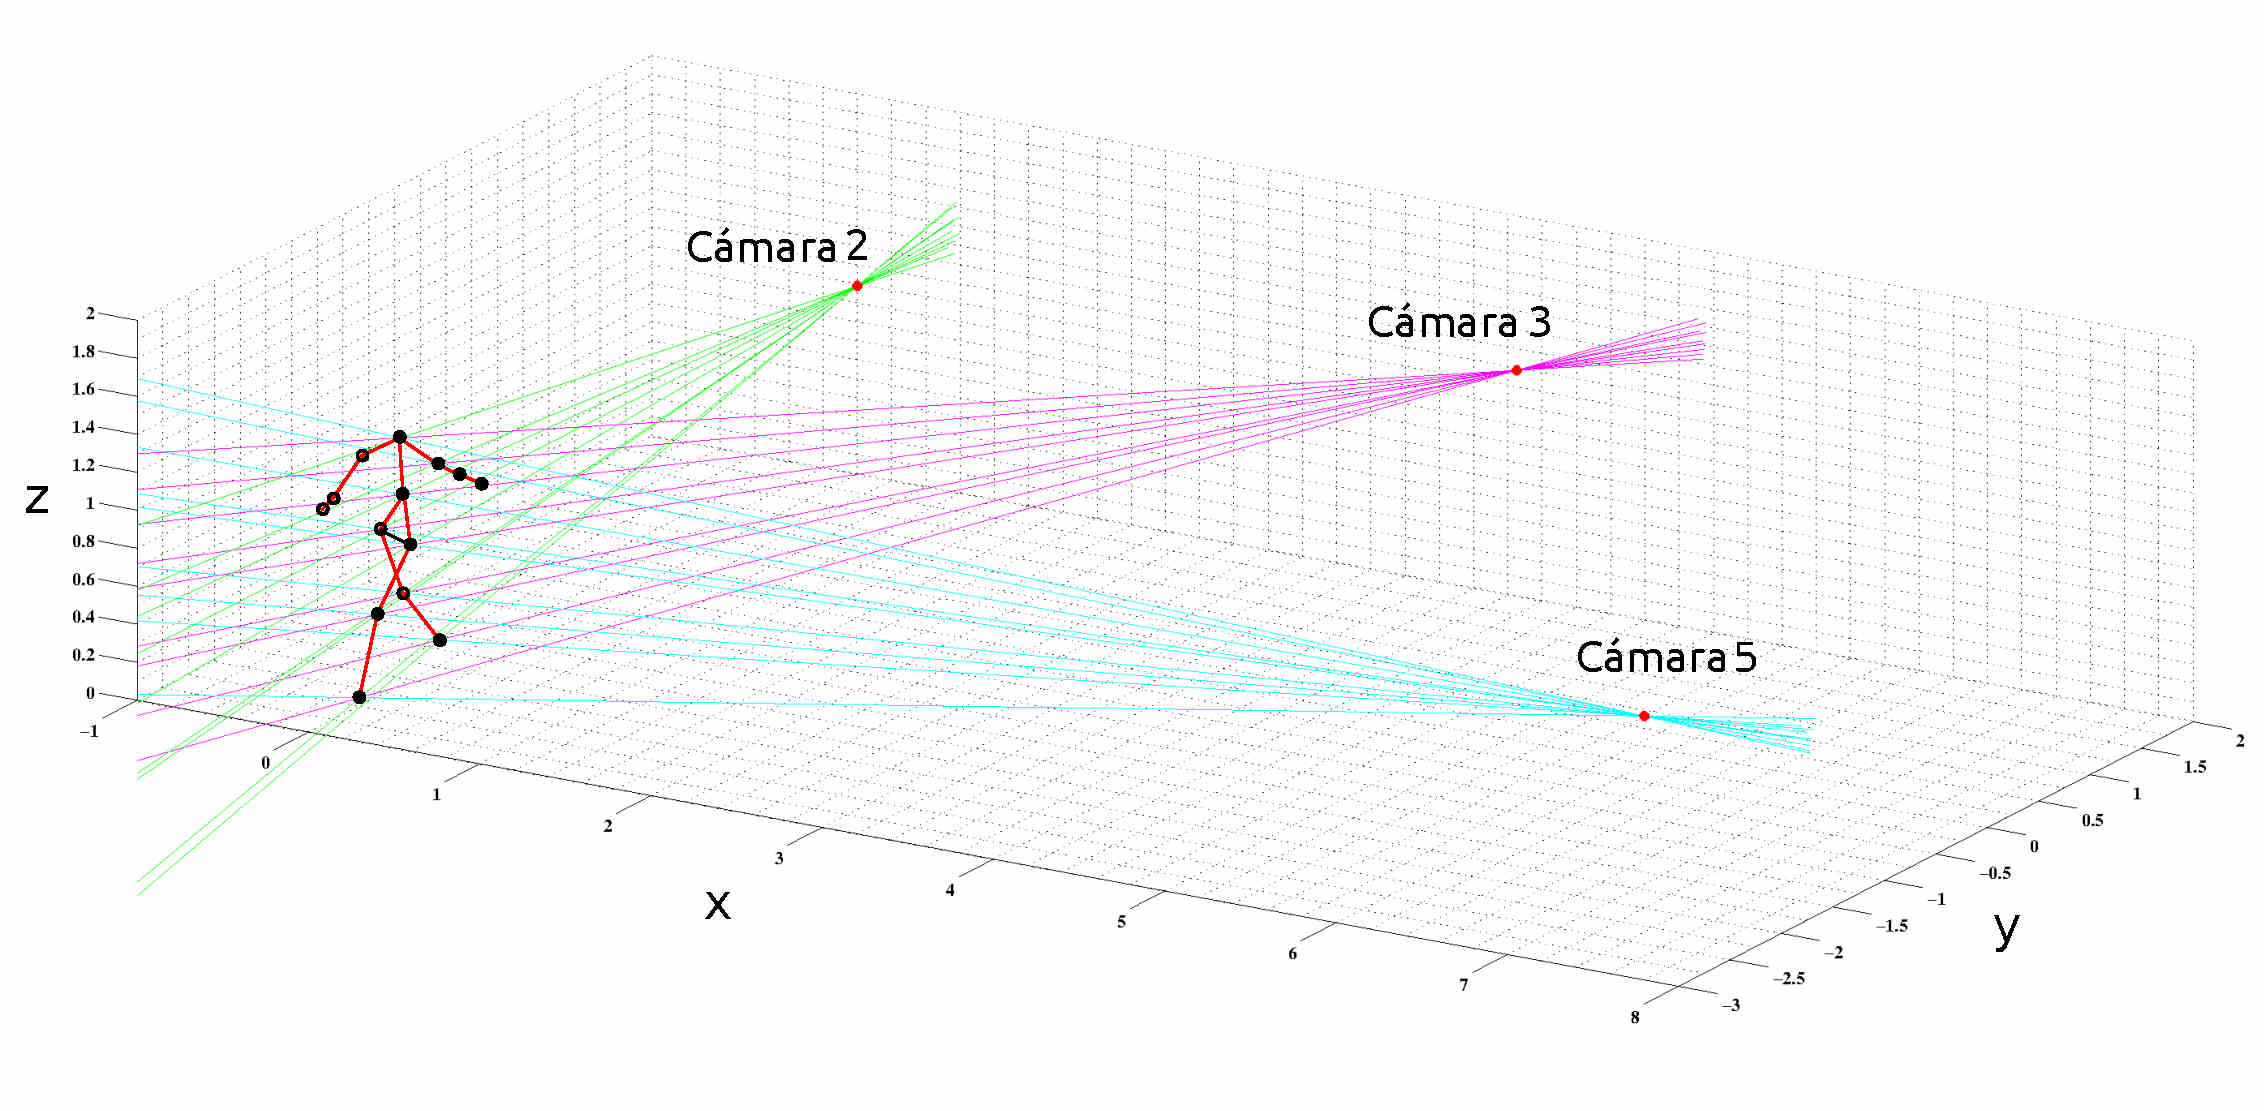
\includegraphics[scale=0.5]{img/Reconstruccion/Reconstruccion_3_camaras2.jpg}
\caption{Ejemplo del proceso de reconstrucción. Los marcadores totalmente negros son los que se pudieron reconstruir utilizando información de las cámaras 2, 3 y 5.}
\end{figure}


Como se menciona previamente se han realizado dos implementaciones distintas del bloque  \emph{Asociar puntos 2D} (Sección \ref{seccion_asociar2D_uno}), que se diferencian en el criterio para seleccionar los pares de cámaras:
\begin{itemize}
\item La primera implementación  considera las asociaciones de marcadores posibles entre pares de cámaras, evaluando cada una de las cámaras respecto a todas las restantes. 
\item La segunda implementación toma en cuenta  la configuración circular de las cámaras en el espacio y se evalúa cada cámara con la que se encuentra inmediatamente más cerca,  recorriendo las cámaras en algún sentido.
\end{itemize}
  

\begin{table}[ht!]
\hspace{-1cm}
\resizebox{15cm}{!} {
\begin{tabular}{cc|c|c|c|c|}
\cline{3-6}
                                                                              &                                                       & \multicolumn{2}{l|}{\textbf{Primera implementación}}                                                                                             & \multicolumn{2}{l|}{\textbf{Segunda implementación}}                                                                                            \\ \hline
\multicolumn{1}{|l|}{\begin{tabular}[c]{@{}l@{}}\textbf{Marker}\\ \textbf{Ground}\end{tabular}} & \begin{tabular}[c]{@{}l@{}}\textbf{Name}\\ \textbf{Ground}\end{tabular} & \begin{tabular}[c]{@{}l@{}}\textbf{Error} \\ \textbf{Promedio}\\ \textbf{(cm)}\end{tabular} & \begin{tabular}[c]{@{}l@{}}\textbf{Percentil}\\ \textbf{99\% (cm)}\end{tabular} & \begin{tabular}[c]{@{}l@{}}\textbf{Error}\\ \textbf{Promedio}\\ \textbf{(cm)}\end{tabular} & \begin{tabular}[c]{@{}l@{}}\textbf{Percentil}\\ \textbf{99\% (cm)}\end{tabular} \\ \hline
\multicolumn{1}{|l|}{1}                                                       & LeftUpLeg                                             & 0.4182                                                           & \textbf{3.7197}                                                        & 0.3671                                                          & 0.5158                                                        \\ \hline
\multicolumn{1}{|l|}{2}                                                       & LeftLeg                                               & 0.3586                                                           & 0.5449                                                        & 0.3670                                                          & 0.5411                                                        \\ \hline
\multicolumn{1}{|l|}{3}                                                       & LeftFoot                                              & 0.3862                                                           & 1.0379                                                        & 0.3720                                                          & 0.5580                                                        \\ \hline
\multicolumn{1}{|l|}{4}                                                       & RightUpLeg                                            & 0.3963                                                           & 1.7542                                                        & 0.3714                                                          & 0.5879                                                        \\ \hline
\multicolumn{1}{|l|}{5}                                                       & RightLeg                                              & 0.3830                                                           & 0.9840                                                        & 0.3780                                                          & 0.5860                                                        \\ \hline
\multicolumn{1}{|l|}{6}                                                       & RightFoot                                             & 0.4192                                                           & 1.5364                                                        & \textbf{0.4212}                                                          & \textbf{1.8483}                                                        \\ \hline
\multicolumn{1}{|l|}{7}                                                       & Spine                                                 & 0.4075                                                           & 0.9092                                                        & 0.4040                                                          & 0.6043                                                        \\ \hline
\multicolumn{1}{|l|}{8}                                                       & Head                                                  & 0.4130                                                           & 1.2853                                                        & 0.3867                                                          & 0.9063                                                        \\ \hline
\multicolumn{1}{|l|}{9}                                                       & LeftArm                                               & 0.3626                                                           & 0.6394                                                        & 0.3666                                                          & 0.7997                                                        \\ \hline
\multicolumn{1}{|l|}{10}                                                      & LeftForeArm                                           & \textbf{0.4774}                                                           & 2.8511                                                        & 0.3873                                                          & 0.9056                                                        \\ \hline
\multicolumn{1}{|l|}{11}                                                      & LeftHand                                              & 0.4217                                                           & 2.0700                                                        & 0.4007                                                          & 1.1722                                                        \\ \hline
\multicolumn{1}{|l|}{12}                                                      & RightArm                                              & 0.4756                                                           & 2.4363                                                        & 0.4025                                                          & 1.4771                                                        \\ \hline
\multicolumn{1}{|l|}{13}                                                      & RightForeArm                                          & 0.4590                                                           & 3.1711                                                        & 0.3844                                                          & 0.7810                                                        \\ \hline
\multicolumn{1}{|l|}{14}                                                      & RightHand                                             & 0.4545                                                           & 2.4782                                                        & 0.3816                                                          & 0.7728                                                        \\ \hline
\multicolumn{1}{l|}{}                                                         & \textbf{Secuencia }                                            & \textbf{0.38556 }                                                         & \textbf{1.7907    }                                                    & \textbf{0.35686}                                                         &\textbf{ 0.81266}                                                       \\ \cline{2-6} 
\end{tabular}
}
\caption{Performance de los algoritmos implementados en reconstrucción. }
\label{table_performance_reconstruccion}
\end{table}

En la Tabla \ref{table_performance_reconstruccion} se muestra una comparación de resultados. En la misma se observa que en la segunda  implementación el error promedio mejora ligeramente respecto a la primera implementación. Se observa también el error considerando el 99\% de los marcadores, donde la mejora de la segunda implementación es más significativa. Por esta razón se ha elegido la segunda de las implementaciones.


Una de las razones por las cuales puede suceder esto, es que en el primer algoritmo se realizan búsquedas de asociaciones entre marcadores detectados, en pares de cámaras donde la probabilidad de que un mismo marcador sea visto por ambas puede ser muy baja. El ejemplo más representativo es cuando se consideran cámaras que están  ubicadas en posiciones diametralmente opuestas. En este caso las asociaciones que se encuentren tienen mayores posibilidades de ser asociaciones incorrectas, influyendo negativamente sobre el desempeño global del algoritmo. 



\section{Resultados de reconstrucción sobre secuencias reales}

Para probar la reconstrucción con secuencias reales se realizó la calibración según lo explicado en la Sección \ref{seccion_calibracion_secuencias_reales}, por otra parte fue necesario robustecer el algoritmo de detección de marcadores como se explica en la Sección \ref{resultadosyanalisissegmentacion}. Las pruebas del algoritmo presentado anteriormente realizadas sobre esta secuencia no han dado resultados aceptables, en este caso la mayoría de los marcadores se reconstruyen erróneamente. 


Con el fin de encontrar donde falla el sistema se genera una secuencia sintética donde se utilizan tres cámaras para la captura. Dichas cámaras están ubicadas en posiciones relativas que simulan el caso real, de esta manera se procede a probar el sistema con dichas secuencias.  En este caso los resultados tampoco han sido aceptables. Tras varias pruebas se llega  a la conclusión de que la deficiencia del sistema es que el algoritmo de reconstrucción, no es lo suficientemente robusto para el caso en que se utilizan pocas cámaras.\\
% % % % % % % % % % % % % % % % % % % % % % % % % % % %
% % % % % %Poner UNA FIGURA DEL RESULTADO MOSTRANDO QUE TAN MALO ES.
% % % % % % % % % % % % % % % % % % % % % % % % % % % % %
Esta situación ha motivado el desarrollo de mejoras sobre este algoritmo. Los cambios se realizan sobre la implementación disponible del sistema, con el fin de lograr un desempeño aceptable sin modificar la estructura global del sistema.

\section{Mejoras del algoritmo de reconstrucción}


Se hicieron pruebas sobre la base sintética, nuevamente simulando la situación del caso real, con el fin de aislar los errores provenientes de la calibración y de la detección de marcadores.
El algoritmo que se implementa en este caso, con el fin de solventar dichos errores, tiene una estructura similar al considerado anteriormente (ver Figura \ref{fig: diagrama algoritmo}), aunque algunos bloques modifican su funcionamiento, fundamentalmente el primero (\emph{Asociar puntos 2D}).

\subsection{Asociar punto 2D}

En esta versión modificada, el resultado de \emph{Asociar puntos 2D} continúa siendo una lista ordenada de asociaciones entre puntos de distintas cámaras, pero el procedimiento para generar dicha lista es diferente. \\  

Para cada punto de una retina se genera una lista ordenada que asocia dicho punto con los puntos de las restantes retinas. El orden de la lista se establece según la distancia euclídea entre los rayos de proyección de los puntos a asociar.\\

De esta forma se obtiene una matriz de distancias entre rayos de proyección 3D. Cada columna de esta matriz es una combinación posible de dos rayos de proyección. Cada fila se compone de la siguiente manera:
\begin{itemize}
\item Número de cámara $\alpha$.
\item Índice del punto 2D cámara $\alpha$.
\item Número de cámara $\beta$.
\item Índice del punto 2D cámara $\beta$.
\item Distancia entre los rayos de proyección de los puntos considerados.
\end{itemize}



\begin{figure}[ht!]
\centering
\captionsetup{justification=centering,margin=2.8cm}
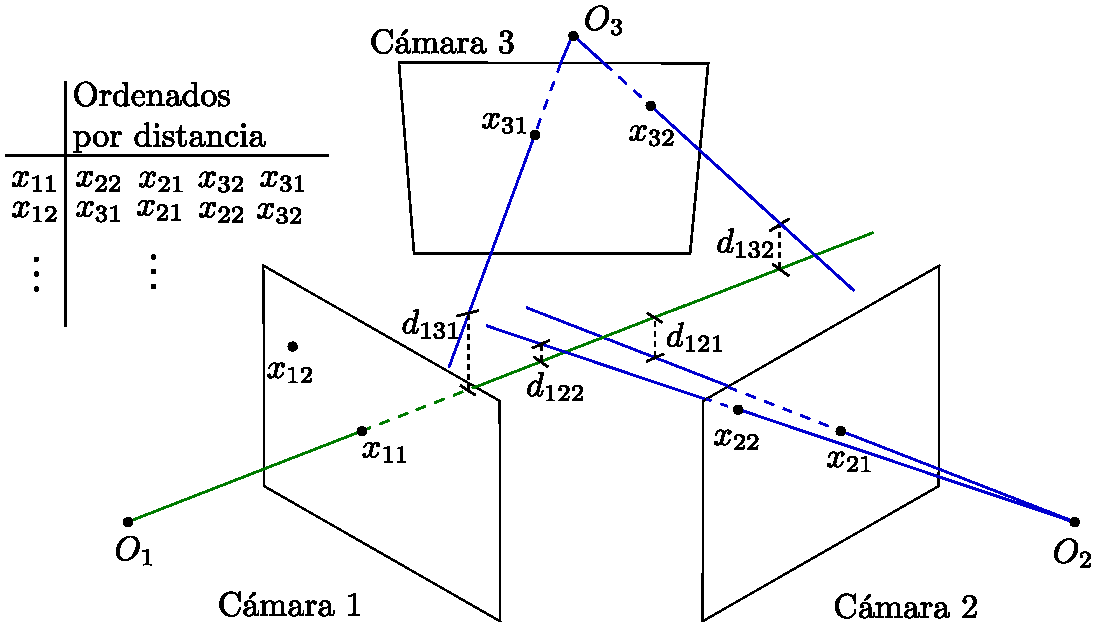
\includegraphics[scale=0.7]{img/Reconstruccion/Asociar_puntos_2}
\caption{Nueva asociación de puntos entre pares de cámaras.}
\end{figure}
 
\subsection{Mejor asociación}


Este bloque mantiene su funcionalidad, encontrar la pareja de puntos entre dos vistas, con mayor probabilidad de corresponder a la proyección de un punto 3D.
La diferencia fundamental con su implementación anterior es la gestión de las matrices de entrada, pues el ordenamiento por distancia de dichas matrices es diferente. 


En la primera implementación las distancias que producen el ordenamiento son generadas entre rectas epipolares y puntos, o sea distancias sobre un plano, mientras que en esta implementación las distancias son entre rayos en el espacio 3D.


Manteniendo el criterio original para implementar este bloque, el cual consiste en tomar la pareja de puntos que genere rayos de proyección con la menor distancia entre sí. 
La nueva entrada proporcionada por \emph{Asociar puntos 2D} simplifica la implementación a desarrollar.


Una vez que se tiene la matriz de distancias con todas las asociaciones de puntos entre los pares de cámaras considerados, este bloque simplemente toma de entre todas las asociaciones disponibles de puntos válidos, aquel par de puntos que posea menor distancia asociada.
Recordar que un punto se considera válido si en iteraciones anteriores no se ha podido asociar a ningún punto 3D reconstruido.

\subsection{Resto de los bloques}

Los bloques de \emph{Reconstrucción 3D y Validación}, y el de \emph{Actualizar Asociaciones} realizan el mismo funcionamiento y tiene igual implementación que los utilizados en el algoritmo anterior (ver Secciones \ref{seccion_reconstruccion3D_validacion} y \ref{actualizar_asociaciones}).

  Asimismo la condición que debe cumplirse para detener el proceso iterativo es la misma.

  
  
\section{Resultados del nuevo algoritmo}  


\begin{figure}[ht!]
   \centering 
    \subfloat[Vista derecha.]{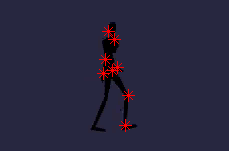
\includegraphics[scale=1.70]{img/Reconstruccion/50_derecha_sintetica.png}}\hspace{0.2cm}
    \subfloat[Vista  izquierda.]{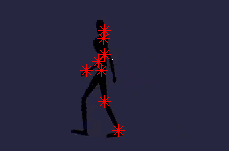
\includegraphics[scale=1.70]{img/Reconstruccion/50_izquierda_sintetica.png}}\hspace{2cm}
    \subfloat[Vista de atras.]{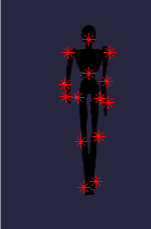
\includegraphics[scale=0.90]{img/Reconstruccion/50_atras_sintetica2.png}} \hspace{1.9cm}
    \subfloat[Resultado de la reconstrucción.]{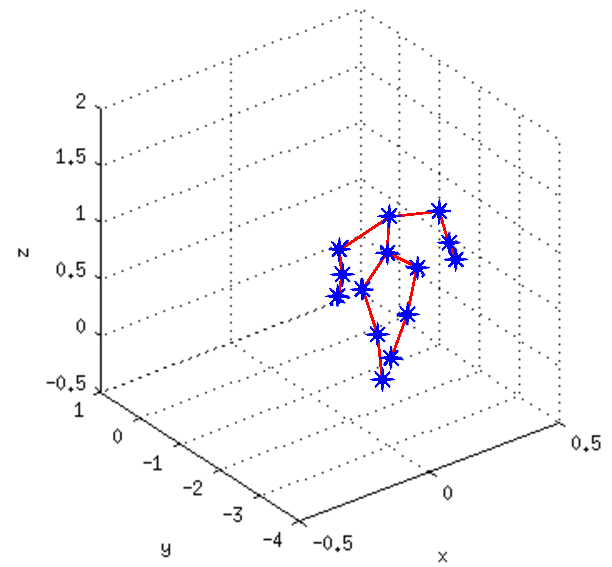
\includegraphics[scale=0.7]{img/Reconstruccion/50_matlab_sintetica.pdf}}    
   \caption{Reconstrucción de una secuencia sintética. Los asteriscos rojos indican los marcadores detectados.} 
   \label{img_reconstruccion_sintetica}    
\end{figure} 

 
Se prueba el nuevo algoritmo para una secuencia sintética de tres cámaras en las que se intenta simular el caso real. En este caso el sujeto cuenta con catorce marcadores. 
Los resultados muestran una mejora significativa respecto al algoritmo original
aunque no se llega a tener un desempeño ideal. 
De 20 cuadros relevados, en 11 de ellos se logra reconstruir de manera aceptable los 14 marcadores, en seis de los cuadros se tiene un marcador incorrectamente reconstruido y en los tres restantes se tiene dos marcadores incorrectamente reconstruidos.
En la Figura \ref{img_reconstruccion_sintetica} se muestra el resultado de la reconstrucción para un cuadro  determinado de la secuencia sintética.

\begin{figure}[ht!]
   \hspace{-1cm}
    \subfloat[Vista derecha.]{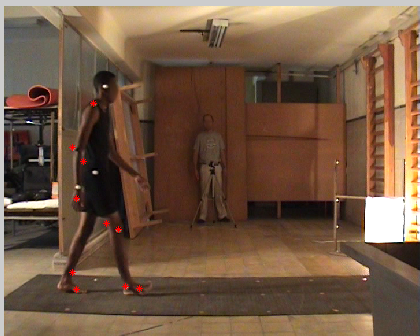
\includegraphics[scale=0.47]{img/Reconstruccion/22_derecha.png}}\hspace{0.3cm}
    \subfloat[Vista de atrás.]{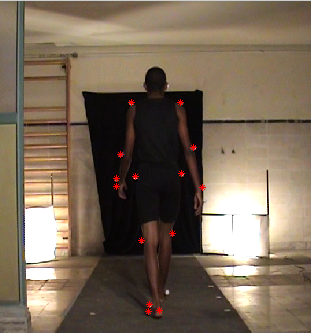
\includegraphics[scale=0.47]{img/Reconstruccion/22_atras.png}}\hspace{2cm}
    \subfloat[Vista izquierda.]{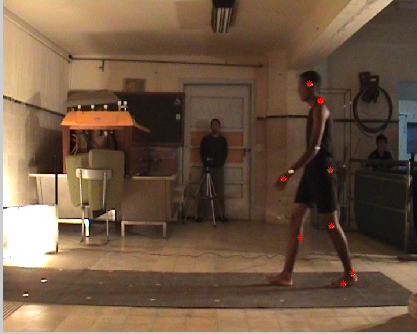
\includegraphics[scale=0.47]{img/Reconstruccion/22_izquierda.png}}\hspace{0.5cm}
    \subfloat[Resultado de la reconstrucción.]{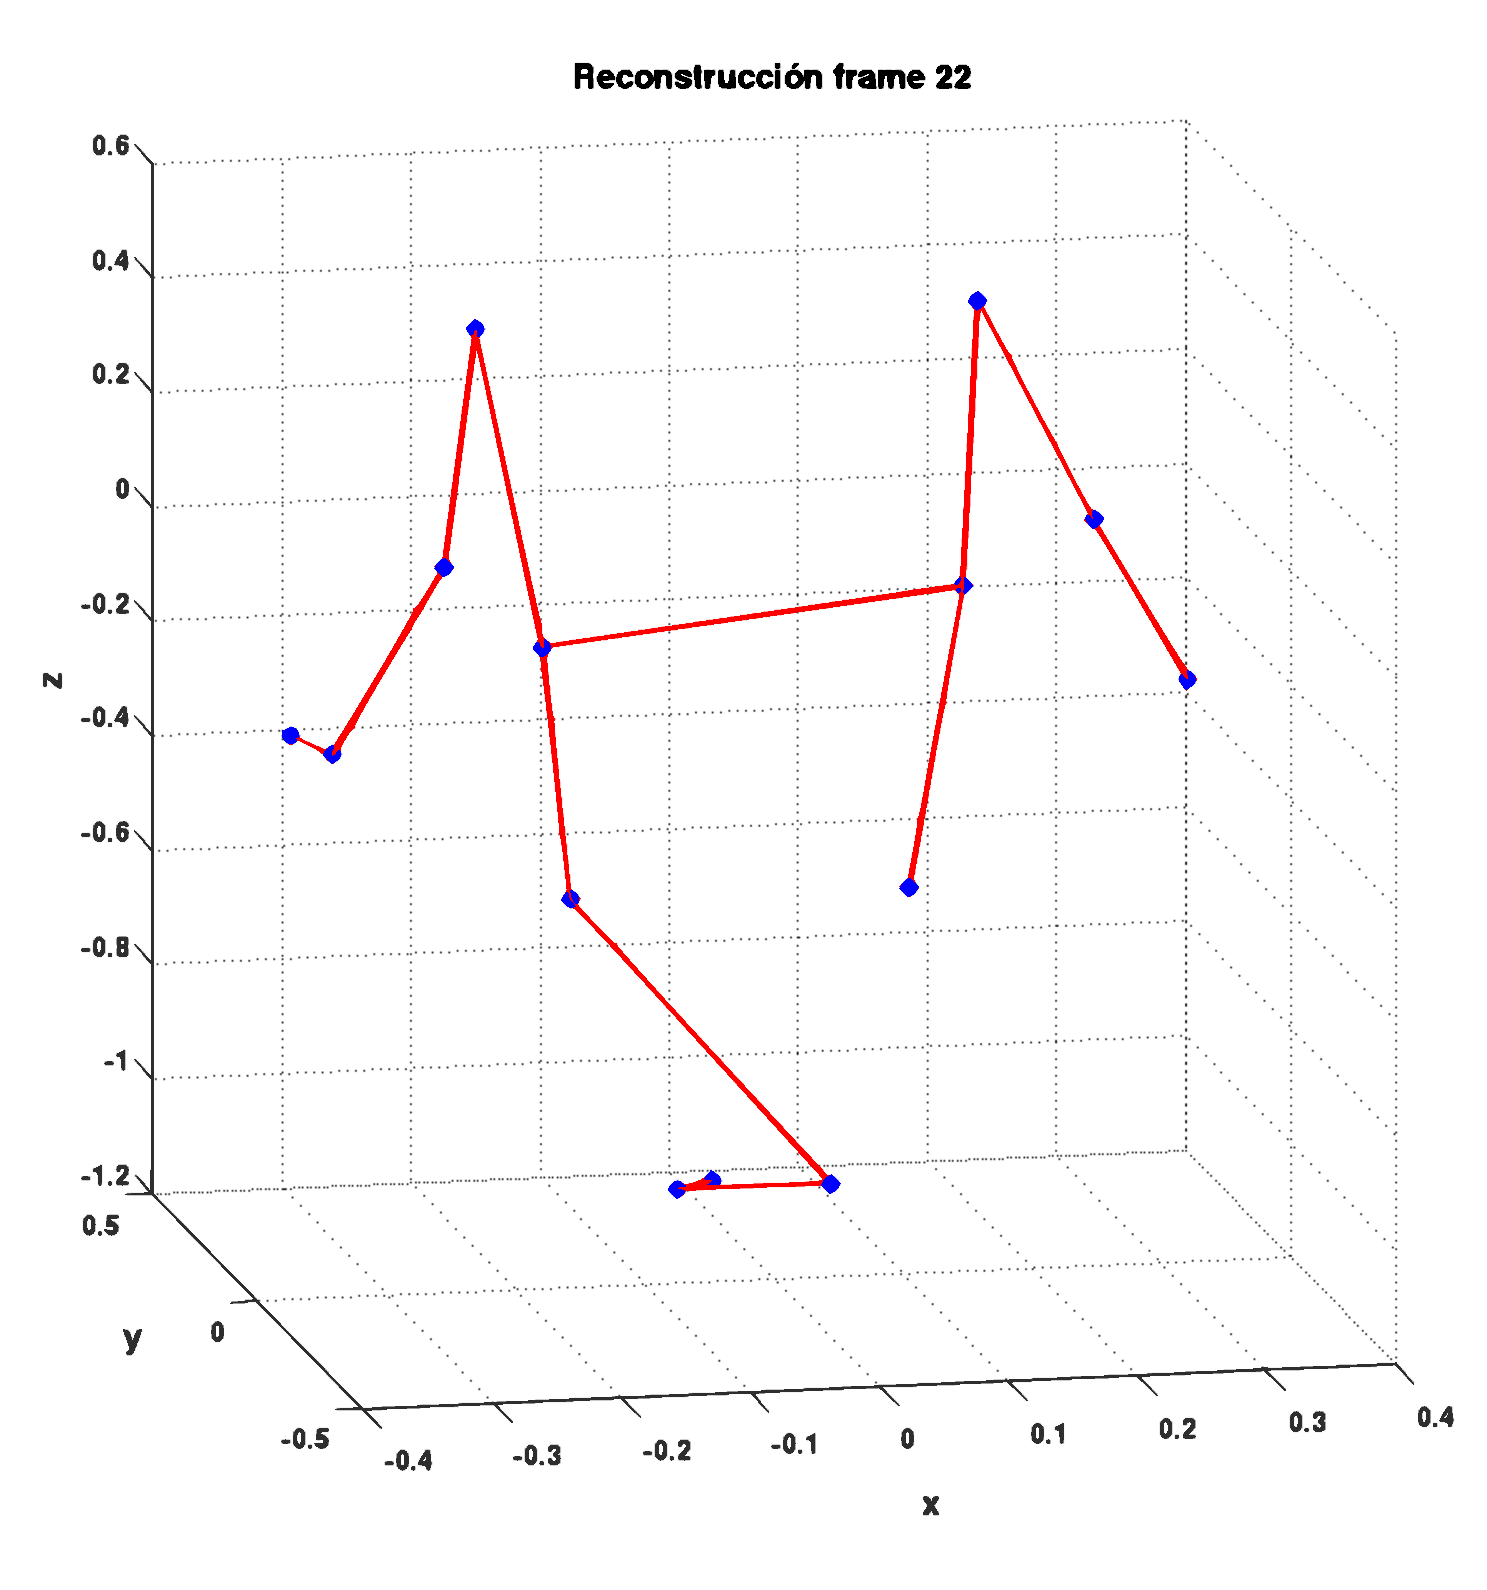
\includegraphics[scale=0.20]{img/Reconstruccion/frame22_esqueleto_armado.pdf}}
   \caption{Reconstrucción de una secuencia real. Los asteriscos rojos indican los marcadores detectados.} 
   \label{img_reconstruccion_real2}    
\end{figure} 

Por último el nuevo algoritmo fue probado con secuencias reales. Si bien se reconstruyen varios marcadores mejorando la performance que se tenía con el algoritmo de reconstrucción inicial, los resultados no son tan alentadores como los obtenidos para las secuencias sintéticas. En cierta manera es esperable dado que en este caso se adicionan errores provenientes de las etapas de detección de marcadores y de calibración. En la Figura \ref{img_reconstruccion_real2} se muestra el resultado obtenido para un cuadro de la secuencia real. 




\section{Conclusión} 

Tomando como punto de partida las ideas propuestas por Herda, referentes a la reconstrucción de puntos 3D a partir de múltiples imágenes de puntos sobre distintas cámaras,  se han diseñado e implementado dos variantes de algoritmo principal para la etapa de reconstrucción. Logrando probar dichos algoritmos sobre secuencias tanto sintéticas como reales se hace un análisis cualitativo de los resultados.\\


Inicialmente se genera un algoritmo con etapas bien definidas (ver Figura \ref{fig: diagrama algoritmo}), que obtiene resultados aceptables para secuencias sintéticas y configuraciones de más de seis cámaras. Como es de esperar la configuración espacial de las cámaras influye en el desempeño del algoritmo, por lo que la afirmación anterior es válida asumiendo una distribución de cámaras uniforme alrededor del espacio de captura.\\


Las pruebas realizadas sobre secuencias reales dejan presente el problema de desempeño que tiene el algoritmo cuando se utilizan pocas cámaras, produciendo resultados poco satisfactorios. 
En este caso, las secuencias reales obtenidas manejan tan solo tres cámaras y las condiciones de laboratorio no son las más favorables para efectuar un proceso de detección adecuado. Se ha visto que es necesario robustecer las etapas tanto de detección de marcadores  como de calibración, pues las incertidumbres producidas en dichas etapas tienen un efecto crítico sobre el desempeño de la reconstrucción. Con las secuencias reales disponibles, la falta de marcadores sobre las cámaras en la etapa de detección, es la mayor dificultad a enfrentar en el proceso de reconstrucción. \\



Con el fin de independizar la reconstrucción de los efectos de etapas anteriores, se introduce una secuencia sintética que simula el caso real, tanto en la calidad del movimiento como en el número y disposición de cámaras, donde los errores de calibración y detección de marcadores no son significativos.


Utilizando esta secuencia se implementa un nuevo algoritmo que mejora el desempeño en secuencias con pocas cámaras. Este nuevo algoritmo modifica parcialmente algunas etapas del algoritmo inicial, sobre todo la etapa de \emph{Asociar puntos 2D}, logrando obtener resultados significativamente mejores al tratar con pocas cámaras sobre el caso sintético.
Utilizando las secuencias reales, se obtiene mejoras cualitativas sobre el primer algoritmo, si bien el desempeño es inferior al caso sintético y la reconstrucción es apenas aceptable.  \\ 


De lo expuesto se desprenden fundamentalmente dos cosas:
\begin{itemize}
\item Las dificultades que ofrece el caso real, básicamente en la detección de marcadores, y cómo influye significativamente en la etapa de reconstrucción perjudicando el resultado final del sistema. Con lo cual se desprende que mejoras en la detección deberían tener un gran impacto en la reconstrucción.
\item El número de cámaras cambia significativamente el problema:
\vspace{-0.3cm}
\begin{itemize}
\item Por un lado se genera un algoritmo que gestiona de manera aceptable la redundancia de información que existe cuando se utiliza un número de cámaras superior al necesario para cubrir cierto espacio de captura (dadas las características de los movimientos tratados en este proyecto, básicamente de marcha rectilínea, el límite inferior para una reconstrucción aceptable son seis cámaras). Cabe recordar en este punto que los sistemas comerciales poseen generalmente como mínimo 8 cámaras e intentan trabajar con redundancia de información.
\item Por otro lado efectuando modificaciones al algoritmo anterior se genera un nuevo algoritmo, que permite trabajar con pocas cámaras pero no gestiona adecuadamente la redundancia de información.
\end{itemize}  
\end{itemize} 

El análisis en biomecánica exige restricciones sobre precisión espacial en los resultados de la reconstrucción, por lo que resulta necesario optimizar esta etapa. 

De lo visto en la bibliografía existente podría proponerse el uso de la información de esqueleto, teniendo presente que esto último, impone restricciones sobre las posiciones de los marcadores y particulariza los casos de uso del sistema. Si bien este tipo de análisis se menciona en el algoritmo propuesto por Herda, se decide en este trabajo generar un algoritmo en principio más general, con entradas y salidas bien determinadas y no se incorpora la información de esqueleto. \\
%VER CON GUILLERMO QUE QUISO PONER EN UNOS COMENTARIOS QUE ME PASO
 
 
 
%
%
%->Reconstrucción con base de datos sintética
%\\
%HABLAR Y MOSTRAR RESULTADOS DE La performance DE LA BASE DE DATOS AL UTILIZAR LAS DOS RAMIFICACIONES\\
%PROCEDIMIENTO DE ASOCIACIONES DEL TIPO TODO CONTRA TODO, Y ASOCIACIONES CON CÁMARAS CONSECUTIVAS.\\
%JUSTIFICAR POR LO TANTO QUE OFICIALMENTE NOS QUEDAMOS CON EL CASO DE ASOCIACIONES ENTRE CÁMARAS CONSECUTIVAS
%\\
%-----\\
%->CASO REAL
%\\
%\begin{itemize}
%\item introducción: SE PRUEBA SOBRE LO QUE SE TIENE DEL SISTEMA Y NO ANDA POR TAL Y TAL MOTIVO. pUES LA CALIBRACIÓN ES DIFERENTE NO SE OBTIENE RESULTADOS ACEPTABLES.
%
%\item EXPLICAR AJUSTE REALIZADOS, GENERACIÓN DE MINI-SISTEMA DONDE CORREN SECUENCIAS REALES.AQUÍ DEBE ESTAR EL NUEVO ALGORITMO DE RECONSTRUCCIÓN
%\begin{itemize}
%\item para todos los puntos contenidos en las retinas se trazan las correspondientes rectas de proyección 3D
%\item BLOQUE ASOCIACIÓN 3D: se asocian las rectas utilizando una métrica de distancia euclídea Las rectas de proyección que se encuentran a menor distancia entre si quedan asociadas.
%\item BLOQUE MEJOR ASOCIACIÓN: se elijen las n mejores asociaciones entre rectas 3D
%\item BLOQUE RECONSTRUCCIÓN: se reconstruyen los puntos 3D provenientes de las asociaciones anteriores 
%\end{itemize}
%
%\item EN DICHO MINI-SISTEMA SE SIMULA EN BLENDER EL CASO REAL Y SE INTENTA TENER ALGO MODERADAMENTE FUNCIONAL
%
%\item RESULTADOS -->ALGORITMO DE RECONSTRUCCIÓN OFICIAL(CASO ASOCIACIÓN ENTRE CÁMARAS CONSECUTIVAS) -->NO TUVO BUENOS RESULTADOS 
%\item CONSECUENCIA SE GENERA NUEVO ALGORITMO DE RECONSTRUCCIÓN QUE HACE TAL Y TAL COSA.
%\item CON ESTE NUEVO ALGORITMO SE OBTIENEN RESULTADOS ACEPTABLES SOBRE LAS SIMULACIONES DEL CASO REAL
%SE PRUEBA DICHO ALGORITMO SOBRE LOS DATOS REALES Y SE OBTIENEN RESULTADOS ACEPTABLES.
%\item JUSTIFICAR QUE LAS DIFERENCIAS SON DEBIDAS A CALIBRACIÓN (REAL VS SINTÉTICA) Y LA SEGMENTACIÓN (REAL VS SINTÉTICA).
%\item ¿CUALITATIVAMENTE SE PUEDE DECIR CUAL ES EL FACTOR QUE PERJUDICA EN MAYOR MEDIDA LOS RESULTADOS en la secuencia real RESPECTO AL CASO DE SIMULACIÓN SINTÉTICA?. Si la segmentación es lo que perjudica más, por tal y tal motivo.
%\end{itemize}
%
%\textbf{HABLAR DE LA INTEGRACIÓN DE ESTE NUEVO ALGORITMO EN EL SISTEMA COMPLETO.\\}
%\begin{itemize}
%\item para muchas cámaras (mas de 5 o 6, ver las pruebas de gonzalo) el sistema funciona razonablemente con la reconstrucción ``original''. Principalmente debido a que se cuenta con información redundante de los marcadores.
%\item para pocas cámaras se utiliza el nuevo algoritmo de reconstrucción, permite trabajar con la secuencia real disponible. con muchas cámaras el algoritmo puede ser computacionalmente complejo.
%\item explicar bien cual es la frontera entre uno y otro caso (5 o 6 cámaras?)
%\end{itemize}




\section{Seguimiento}

\subsection{Introducción}

La salida del bloque de reconstrucción, son los puntos 3D generados a partir de los múltiples vídeos de cada vista, presentados en el orden que fueron validados en cada frame (figura \ref{reconstr_00}). A su vez, los marcadores fueron reconstruidos tomando como entrada los puntos obtenidos en las imágenes de la segmentación, no teniendo estos información alguna sobre el cuerpo, mas que el orden en el que son generados al segmentar.

Son presentados sin orden definido para cada cuadro de la secuencia, y el objetivo del tracking o seguimiento, es identificarlos temporalmente, asignándoles una etiqueta constante a lo largo de la secuencia para cada marcador y obtener las trayectorias 3D.

\begin{figure}[hbt]
\begin{center}
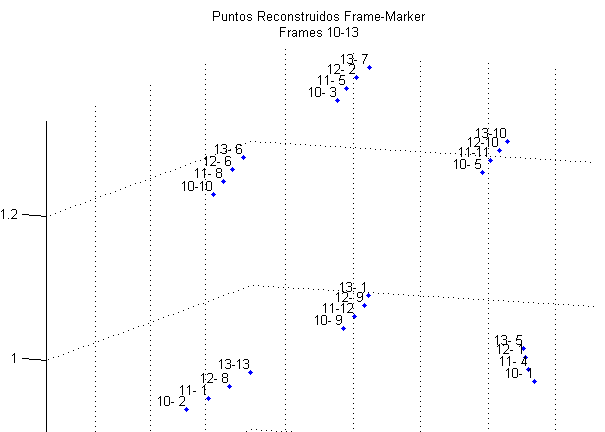
\includegraphics[scale=0.8]{img/Tracking/00_Salida_Reconstruccion.png}
\end{center}
\caption{Salida de Reconstrucción para 4 frames. La etiqueta para cada marcador es el frame y el indice en la reconstrucción}
\label{reconstr_00}
% Figura tomada de la reconstruccion 8_07_100_200
\end{figure}

\subsection{Estado del Arte}

El problema del seguimiento de marcadores espaciales a lo largo del tiempo es un tema de estudio habitual con distintos enfoques, entre ellos:

\begin{itemize}

\item Aplicación de restricciones al movimiento, teniendo información previa de los marcadores a estudiar, como se mueven, y como se relacionan entre ellos. 

\item Predictores Lineales o Estadísticos, teniendo información previa de una trayectoria para estimar el próximo elemento y confirmar o corregir la continuación de la secuencia.

\end{itemize}

Estos enfoques no son mutuamente excluyentes, pudiendo ser ambos complementarios para robustecer la generación de las trayectorias. Si se tiene acceso durante la adquisición de los datos, es posible relevar las distancias entre marcadores que se colocan en miembros que se mueven solidariamente  o dependen directamente uno del otro, por ejemplo al colocar marcadores en articulaciones de los brazos hay elementos sobre los huesos que siempre tendrán la misma distancia entre ellos (salvo una tolerancia, recordando que los marcadores no se encuentran en la articulación misma, sino sobre un lugar representativo sobre el cuerpo como se observa en el ajuste presentado en la figura \ref{skeleton_fitting_herda} , del ajuste planteado en el trabajo \cite{herda}. ). Con estas distancias relevadas y definidas las relaciones entre marcadores, es posible definir el esqueleto como una serie de restricciones que se mantienen a lo largo del tiempo (distancias entre marcadores solidarios) o varían de forma continua (angulo de huesos), donde la identificación es realizada inicialmente mediante un ajuste de los datos relevados en el mundo físico a los puntos obtenidos en la reconstrucción. 

\begin{figure}[hbt]
\begin{center}
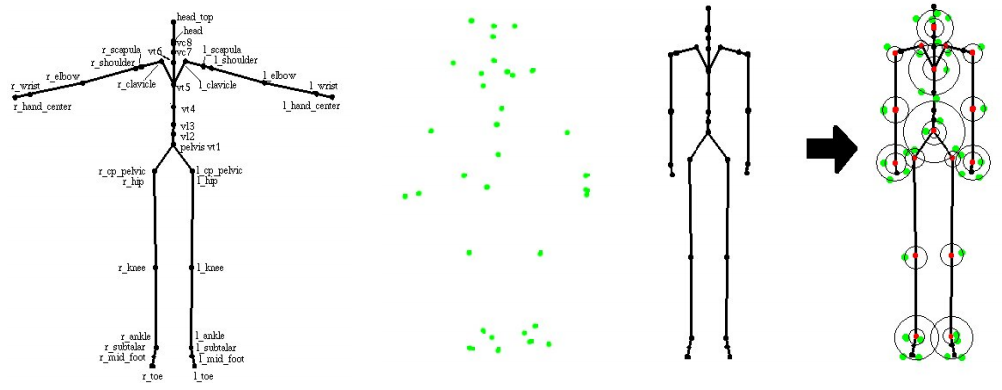
\includegraphics[scale=0.5]{img/Tracking/01_skeleton_fitting_Herda.png}
\end{center}
\caption{Inicializacion de esqueleto, y ajuste a los marcadores encontrados. Cada marcador representa una articulación y se ajusta en una esfera de cercanía centrada en la articulación del esqueleto}
\label{skeleton_fitting_herda}
\end{figure}.

Uno de los algoritmos mas simples \cite{survey_tracking}, es continuar una secuencia buscando el marcador mas cercano al ultimo punto conocido imponiendo la restricción que el traslado es mínimo ("greedy matching"), pero es susceptible a errores para casos muy simples, como se observa en el ejemplo de la figura \ref{greedy_matching} .

\begin{figure}[hbt]
\begin{center}
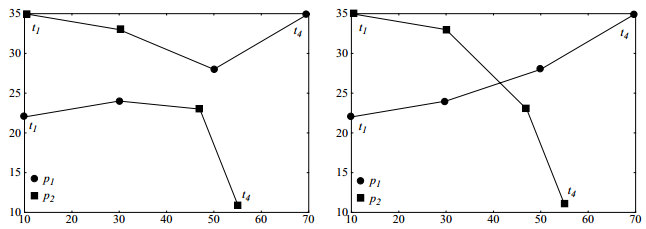
\includegraphics[scale=0.8]{img/Tracking/01_Greedy_Matching.png}
\end{center}
\caption{Dos marcadores moviéndose en cuatro frames, Izquierda corresponde al resultado de aplicar enlazado por elemento mas próximo \cite{survey_tracking} , Derecha al elegir el camino con variación mas suave}
\label{greedy_matching}
\end{figure}.

Para el caso de algoritmos de predicción, algunas soluciones implementadas para el tracking de marcadores son el filtro de Kalman \cite{kalman}, y sus variantes los cuales requieren inicializar y ajustar parámetros internos. Estos fueron implementados en las primeras instancias del estudio del problema, pero se decidió implementar otro procedimiento que sepa corregir los errores del método mas simple, no requerir estudio de parámetros internos para el filtrado, e ingrese alguna restricción a las trayectorias enlazadas.

El procedimiento elegido es el presentado por Lorna Herda\cite{herda} , y consiste en aplicar el tracking de partículas esbozado por Malik,Dracos,Papantoniou \cite{griegos} al seguimiento de marcadores. Este consiste en buscar el desplazamiento de un marcador desde el cuadro [f] al cuadro siguiente [f+1], sobre una ventana de cuatro cuadros.

La hipótesis principal de este algoritmo, es que el muestreo del movimiento capturado es suficiente para que el desplazamiento entre cuadros sea mínimo en distancia, y la idea para predecir y buscar el desplazamiento entre [f] y [f+1], es utilizar la información que se tiene de la secuencia entre [f-1] y [f], y utilizar una segunda proyección entre [f+1] y [f+2] para confirmar el enlace encontrado en el caso que exista mas de una posibilidad (figura \ref{herda_00}).

Para poder confirmar una trayectoria de 4 puntos, se debe cumplir que la misma presenta la menor variación de aceleración para la opción elegida entre todas las posibles, calculada como:

\begin{equation}
\begin{split}
\Delta{a}&= \left| \boldsymbol{\overrightarrow{a}}_{[f][f+1][f+2]}-\boldsymbol{\overrightarrow{a}}_{[f-1][f][f+1]} \right| \\
&= \left| \left(\boldsymbol{\overrightarrow{v}}_{[f+1][f+2]}-\boldsymbol{\overrightarrow{v}}_{[f][f+1]}\right).\Delta{t}-\left(\boldsymbol{\overrightarrow{v}}_{[f][f+1]}-\boldsymbol{\overrightarrow{v}}_{[f-1][f]}\right).\Delta{t} \right| \\
&= \left|\left( x_{[f+2]} - 3.x_{[f+1]} + 3.x_{[f]} - x_{[f-1]} \right).\Delta{t}^2\right|\\
\end{split}
\label{track_var_acc}
\end{equation}

, donde $x_{[f+1]}$ a su vez, es aquel punto de [f+1] que mejor se aproxima al desplazamiento en frames anteriores, minimizando la ecuación \ref{track_acc} 

\begin{equation}
\begin{split}
\boldsymbol{\overrightarrow{v}}_{[f][f+1]}& = \boldsymbol{\overrightarrow{v}}_{[f-1][f]} \\
x_{[f+1]}-x_{[f]}& = x_{[f]}-x_{[f-1]} \\
\end{split}
\label{track_acc}
\end{equation}

\begin{figure}[hbt]
\begin{center}
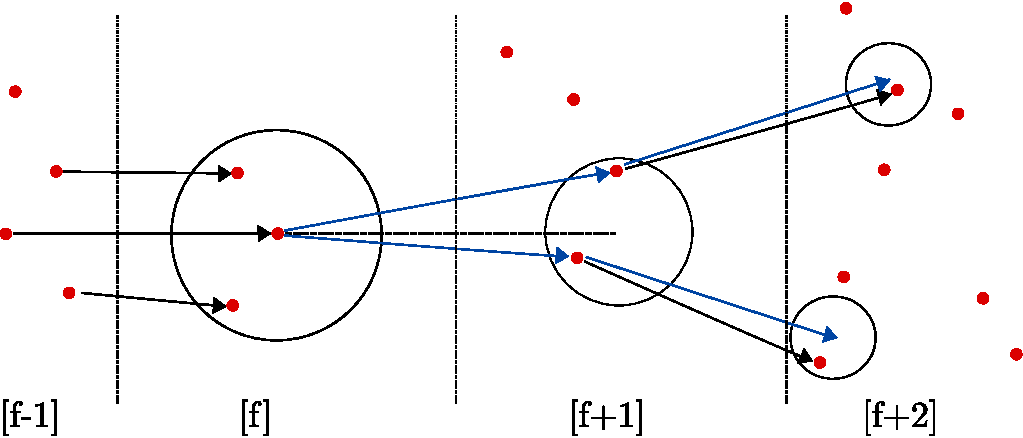
\includegraphics[scale=0.8]{img/Tracking/tracking-eps-converted-to.pdf}
\end{center}
\caption{Seguimiento en 4 frames, siendo [f] el frame actual que queremos seguir en [f+1]. La linea punteada es la traslación del movimiento previo, las lineas azules son las obtenidas buscando la mínima variación de aceleración para el punto elegido en [f+1]. De las dos posibles trayectorias, se elige aquella con menor variación de aceleración}
\label{herda_00}
\end{figure}

En su trabajo\cite{herda}, Lorna Herda propone que realizar el seguimiento sobre la reconstrucción 3D presenta menos continuidad en las trayectorias , con respecto al seguimiento realizado sobre el conjunto de segmentación sumada a la proyección de los puntos reconstruidos 3D en cada vista 2D. Sin embargo, en nuestras pruebas, nos pareció mas coherente trabajar con el seguimiento en los puntos reconstruidos en 3D, ya que en caso de trayectorias que se cruzan en una vista 2D, son fácilmente separadas en 3D debido a la geometría.

Adicionalmente, la reconstrucción fue implementada de forma distinta a la propuesta por Herda, si bien es posible obtener los puntos proyectados en cada vista, no cumplen el mismo rol. Sin implementar la re-proyección, en el tracking sobre una vista individual se pierden trayectorias cuando se pierden de vista como se observa en la figura \ref{tracking_2D_cam_07} .

\begin{figure}[hbt]
\begin{center}
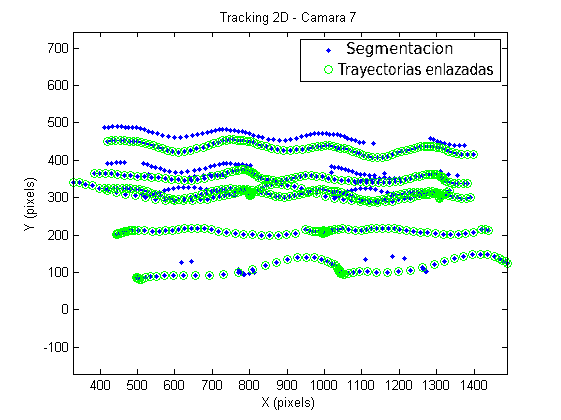
\includegraphics[scale=0.7]{img/Tracking/011_tracking_2D_camara_07.png}
\end{center}
\caption{Resultado de Aplicar el Seguimiento de marcadores a una vista 2D sin reproyección de puntos reconstruidos. Verde, las trayectorias que se enlazaron completamente, Azul los puntos segmentados en la vista 2D de la cámara 07 de la captura sintética}
\label{tracking_2D_cam_07}
\end{figure}

Finalmente, asumiendo que los puntos obtenidos directamente de las animaciones ,proyectados en cada cámara, son el mejor caso de puntos 2D, no presentaban grandes ventajas de trabajar el enlace en cada una de estas vistas 2D, sobre trabajar en 3D posteriormente a la reconstrucción, y no volver hacia atrás ya que la geometría entre vistas cumplió su cometido. Esto ultimo no se cumple para el caso que se evalúen medidas adicionales para robustecer la salida del tracking (por ejemplo, validación por visibilidad, un punto observado en la segmentación de una vista es descartado en caso de no ser físicamente posible ver ese punto entre el cuerpo y la cámara).

\subsection{Implementación}

Para un frame [f] y un marcador $m_{i}^{[f]}$, se desea encontrar en el frame [f+1] el marcador $m_{j}^{[f+1]}$ que continúe la trayectoria que se tiene hasta el momento, cumpliendo las ecuaciones de continuidad \ref{track_acc} y \ref{track_var_acc}. El elemento que traslada la información de un frame al siguiente y desde el anterior, es la matriz de enlaces, donde cada linea es un enlace, y cada enlace tiene los siguientes elementos:
\begin{equation}
\begin{bmatrix}
  m_{h}^{[f-1]} ,\quad m_{i}^{[f]} ,\quad m_{j}^{[f+1]} ,\quad m_{k}^{[f+2]} ,\quad \left|\boldsymbol{\overrightarrow{a}}_{[f-1][f][f+1]}\right| ,\quad \left|\boldsymbol{\overrightarrow{v}}_{[f][f+1]}\right|
\end{bmatrix}
\end{equation}

Para el ejemplo presentado en la figura \ref{reconstr_00} , en frame $f=11$ el marcador $m=8$ presenta el siguiente enlace hacia $(f+1)=12$, 

\begin{equation}
\begin{bmatrix}
  m_{3}^{[10]} ,\quad m_{8}^{[11]} ,\quad m_{3}^{[12]} ,\quad N/A ,\quad \left|\boldsymbol{\overrightarrow{a}}_{[10][11][12]}\right| ,\quad \left|\boldsymbol{\overrightarrow{v}}_{[1][12]}\right|
\end{bmatrix}
\end{equation}

, donde el indice en [13] no aplica debido a que no fue necesario para establecer en enlace entre [11][12].

Al final de cada iteración, la matriz de enlaces es consolidada para asignarle a cada nuevo marcador en [f+1] la etiqueta definida en el primer cuadro del enlazado, la cual puede ser inicializada como texto, si se le presenta la opción al usuario (en caso contrario, se utiliza el orden de los marcadores en el primer frame). Esta asignación será la que se utilice a lo largo de todo el seguimiento, por lo que todo marcador que no sea reconstruido en los primero frames, salvo de tomen medidas adicionales, no aparecerán en las trayectorias finales.

\subsubsection{Enlazado en régimen, inicial y final}

Dado un frame [f], se cargan todos los marcadores de los frames [f-1],[f],[f+1],[f+2], los cuales son puntos en coordenadas cartesianas $X,Y,Z$ (si el seguimiento desea hacerse para una vista 2D, se establece la tercer coordenada de todos los puntos en 1) en unidades correspondiente al plano donde se trabaja (pixeles para vistas 2D, metros para espacio 3D). Dentro de cada frame, los marcadores son identificados según su indice en la reconstrucción, y los enlaces de cada marcador [f-1][f], son cargados a partir de la matriz de enlace del frame anterior (la segunda y tercer columna de la matriz de enlace de [f-1], presenta los mismos datos que la primer y segunda columna de la matriz de enlace en [f], salvo el orden en que es presentada que es asociado al frame en curso).

Para el $i$-esimo marcador en [f], se relevan los indices que componen el enlace [f-1][f] para obtener el traslado previo, y aplicarlo para obtener el centro de búsqueda para el marcador en [f], cumpliendo la ecuación \ref{track_acc} .

\begin{equation}
\begin{split}
\boldsymbol{\overrightarrow{v}}_{[f][f+1]}^{i} = \boldsymbol{\overrightarrow{v}}_{[f-1][f]}^{i} \Rightarrow C_{[f+1]}^{i} &= x_{[f]}^{i} + \boldsymbol{\overrightarrow{v}}_{[f-1][f]}^{i}.\Delta{t} \\
&= 2.x_{[f]}^{i} -x_{[f-1]}^{i} 
\end{split}
\label{centro_busqueda_f1}
\end{equation}

La norma de este traslado es utilizada para evaluar los puntos cercanos al centro de búsqueda, donde pueden surgir tres casos:

\begin{itemize}
\item Se encuentra un solo punto dentro del radio de búsqueda , se agrega el indice del punto encontrado en [f+1] a los que se utilizaron de [f-1] y [f], calculando la aceleración y velocidad resultante para establecer el enlace. En este caso, el cuarto elemento de la linea de la matriz de enlace, no fue necesario 
\item Se encuentra mas de un punto, por lo cual se tiene que usar algún criterio para elegir entre todas la posibilidades encontradas. Para cada punto encontrado dentro del radio de búsqueda, se calcula un segundo centro de búsqueda para [f+2], esta vez minimizando la ecuación \ref{track_var_acc} :
\begin{equation}
\begin{split}
\boldsymbol{\overrightarrow{a}}_{[f][f+1][f+2]}=\boldsymbol{\overrightarrow{a}}_{[f-1][f][f+1]} \Rightarrow C_{[f+2]}^{i} &= x_{[f+1]}^{i} + \boldsymbol{\overrightarrow{v}}_{[f][f+1]}^{i}.\Delta{t} + \boldsymbol{\overrightarrow{a}}_{[f-1][f][f+1]}^{i}.\Delta{t}^2\\
&= 3.x_{[f+1]}^{i} - 3.x_{[f]}^{i} + x_{[f-1]}^{i}\end{split}
\label{centro_busqueda_f2}
\end{equation}
, siendo el radio de búsqueda en [f+2], la distancia [f][f+1]. Con los puntos encontrados en cada búsqueda de todas las posibilidades, se evalúa la variación de aceleración para los puntos [f-1][f][f+1][f+2], y elige la menor de todas, estableciendo el enlace de 4 puntos. Finalmente, se calcula la aceleración y velocidad del enlace [f-1][f][f+2], y se guardan los indices que permitieron la decisión, esta vez con cuatro elementos para indicar que se procedió con la segunda búsqueda.
\item No se encuentra ningún punto, tanto para la búsqueda en [f+1] como en [f+2]. En este caso, se presentan múltiples alternativas, en distintas etapas. La mas inmediata durante el enlazado frame a frame, es aumentar el radio de búsqueda (por ejemplo puede suceder con un punto acelerando y fuera del radio de búsqueda). Este aumento puede ser limitado, o indefinido hasta encontrar un punto aunque en una distancia mucho mayor a la esperada, por lo que deben ser validados posteriormente. Si el enlace pasa la validación dentro del frame, puede no pasar una validación posterior de trayectoria lo que se verá mas adelante
\end{itemize}

El enlazado final es similar a los presentado para régimen, pero en caso de múltiples marcadores candidatos en el frame final [f+1], no se puede extender el movimiento, por lo que se elige mediante menor aceleración en los últimos tres frames con una sola búsqueda desde [f] a [f+1], pero otra alternativa igualmente valida hubiera sido buscar sobre los últimos cuatro frames. Se eligió la primer opción debido a  ser un caso simplificado del enlazado en régimen ya implementada. 

Sin embargo, el enlazado inicial presenta una situación diferente, no se tiene información previa, y deben establecerse las bases para el inicio del enlazado. Para ello se cargan todos los marcadores en los primeros 3 frames, se calculan todas las posibles combinaciones de trayectorias entre elementos. En caso de existir combinaciones forzadas invalidas, las mismas presentan una aceleración resultante notoriamente mayor a la de enlaces, pero si corresponden a algún punto erróneo este se perderá naturalmente durante el enlazado,

Una vez enlazado el ultimo frame de las secuencia, se procede a limpiar aquellas trayectorias que perdieron marcadores en el camino estableciendo un umbral de perdida aceptables sobre el largo de las secuencias obtenidas. Adicionalmente, se descartan todos los puntos reconstruidos que no fueron asignados a ninguna trayectoria 


\subsubsection{Validación e Inventario de trayectorias}

Antes de consolidar la matriz de enlaces y proceder a que los marcadores en [f+1] hereden las etiquetas de las trayectorias a las que pertenecen, los enlaces deben ser validados en múltiples instancias:

\begin{itemize}
\item \textbf{Validación dentro del frame}: verificar que los indices de la matriz de enlaces en [f+1] son únicos, asociados a una sola trayectoria. Si dos o mas trayectorias se enlazaron a un mismo punto en [f+1], se comparará la aceleración con la que fueron enlazadas, validando aquella con menor aceleración, y descartando las otras. En este punto , existe la posibilidad de haber agregado todas las trayectorias involucradas en la decisión en vez de una sola trayectoria por marcador en [f+1], que mejor cumplía las condiciones para ese marcador. De haber elegido esta opción, el descartar una trayectoria que podría haber sido elegida por menor variación , daría paso a la siguiente mejor. Este caso sucedía mas en los casos que se aplico el seguimiento para trayectorias 2D, no tanto en 3D, por lo cual se terminó procediendo con solo una trayectoria por marcador, la cual en caso de ser invalida debe ser evaluada en la etapa de inventario de trayectorias  
\item \textbf{Validación en trayectoria}: pueden existir puntos que fueron reconstruidos con leves errores que deben detectarse, corregirse y estimar un reemplazo. Estos puntos son detectados como enlazados correctamente, pero con posición, velocidad, o aceleración que presenta una discontinuidad notoria, como puede observarse en el ejemplo de la figura \ref{discontinuidad_tracking} ,

\begin{figure}[H]
 \centering
  \subfloat[Trayectoria]{
   \label{track_m13}
    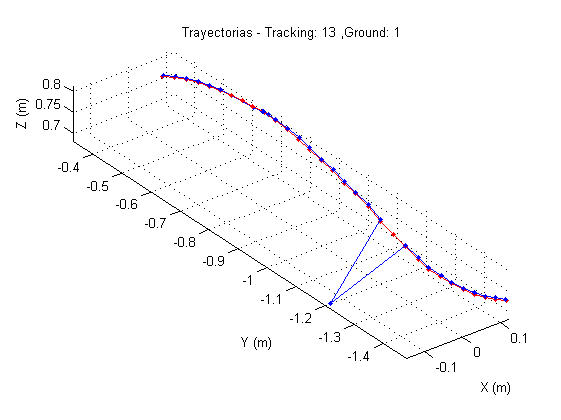
\includegraphics[width=0.5\textwidth]{img/Tracking/025_Salida_Tracking_Marker_13_8_07_100_200.png}}
  \subfloat[Velocidad,Aceleración,Variación Ac.]{
   \label{vel_acc_vacc_m13}
    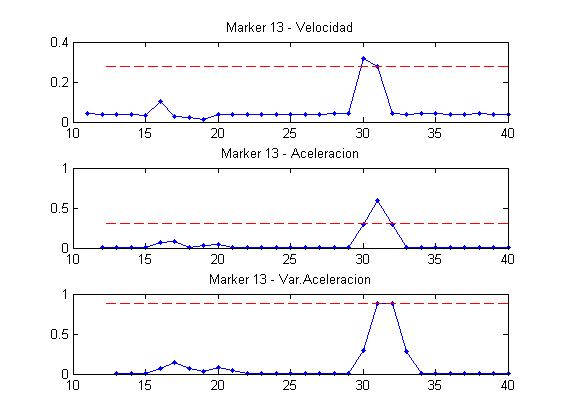
\includegraphics[width=0.5\textwidth]{img/Tracking/020_Salida_Tracking_Marker_13_8_07_100_200.png}}
 \caption{Ejemplo de discontinuidad en un marcador, por punto mal reconstruido. La figura \ref{track_m13} presenta en azul la trayectoria reconstruida, en rojo el ground truth}
 \label{discontinuidad_tracking}
\end{figure}

Se establece un umbral a partir del estudio de la distribución de la aceleración de cada marcador (figura \ref{distribucion_aceleracion} ) para encontrar la aceleración que presenta un salto abrupto, y detectar los frames donde se supera dicho umbral para corregir el marcador. El procedimiento para estimar los marcadores en estos casos, es el mismo que se verá al momento de inventario de trayectorias. 

Como opción mas global, se implementó una alternativa que en vez de calcular un umbral para cada trayectoria, establece un umbral global, el cual es útil para detectar aceleraciones notoriamente altas sin tener que estudiar cada trayectoria. Esta opción se implementó mediante una ejecución en dos instancias del seguimiento, una primera instancia sin limites globales de aceleración en en enlazado, y una segunda con un limite establecido a un porcentaje de la distribución de la aceleración, asumiendo un nivel a priori para perdidas (en nuestras pruebas, se estableció que filtrar al nivel que cumplan el 99\% de las aceleraciones de todos los marcadores enlazados arroja buenos resultados). Si durante la segunda instancia, un enlace global supera este umbral, se descarta y se procede con la recuperación de trayectoria.

\begin{figure}[H]
 \centering
  \subfloat[Función de distribución de la Aceleración]{
	\label{distribucion_aceleracion}
	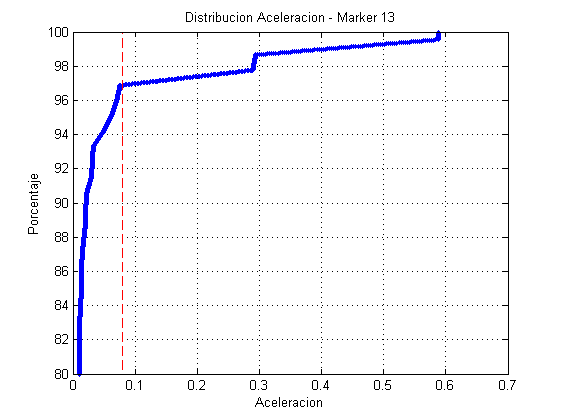
\includegraphics[width=0.5\textwidth]{img/Tracking/03_Distribucion_Aceleracion_Marker_13_8_07_100_200.png}}
  \subfloat[]{
   \label{track_m13_fix}
    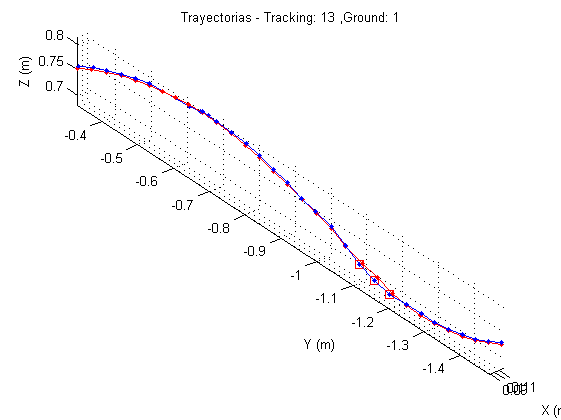
\includegraphics[width=0.5\textwidth]{img/Tracking/026_Salida_Tracking_Marker_13_8_07_100_200.png}}
 \caption{Ejemplo Resultado de Umbral y Corrección En Trayectoria}
% Figura tomada de la reconstruccion 8_07_100_200
\label{distro_acc_track_m13_fix}
\end{figure}
\item \textbf{Inventario de Trayectorias}: Durante el enlazado en un frame, se tienen marcadores en [f] que no lograron enlazarse en [f+1], pero cuya trayectoria podría estar enlazada hasta este frame.
Estos puntos deben ser identificados, mediante la comparación de la segunda columna de la matriz de enlaces [f][f+1] (actual) y la tercer columna de la matriz de enlaces [f-1][f] (anterior), ya que ambas tienen información de los marcadores en el mismo frame, pero enlazan hacia atrás y adelante.
Los elementos que se encuentren en la matriz [f-1][f] , pero no hayan sido enlazados en [f][f+1], son agregados a una lista que  contiene hasta que momento el frame mantenía el enlace (ultima vez que se tuvo información de la trayectoria a la cual pertenece), y que indice de marcador tenia en ese momento (pasar de indice en un frame, a trayectoria a la cual pertenece es trivial consultando las etiquetas de marcador que se van heredando de frame a frame).

Una vez actualizada la lista de las trayectorias perdidas en [f][f+1], se deben tratar de enlazar los puntos de [f+1] que no entraron en el enlazado regular, con las trayectorias perdidas hasta [f-1]. Todos los puntos que sobraron en el enlazado regular, son evaluados contra la lista de trayectorias perdidas, y se revisan dos condiciones:

\begin{enumerate}
  \item \textbf{Distancia con respecto a una estimación lineal}, prolongando el movimiento tomando el ultimo punto como inicio, y los últimos frames de la trayectoria conocida como desplazamiento. El desplazamiento es repetido tantas veces como tiempo perdido tiene el marcador: si una trayectoria estaba definida hasta [f-1] y se buscan enlaces con elementos de [f+1], el desplazamiento es repetido dos veces, como puede observarse en el ejemplo de la figure \ref{track_m8_recover}. 
 
\begin{figure}[H]
 \centering
  \subfloat[Salida de Código durante perdida y recuperación de trayectoria]{
	\label{track_m8_recover_code}
	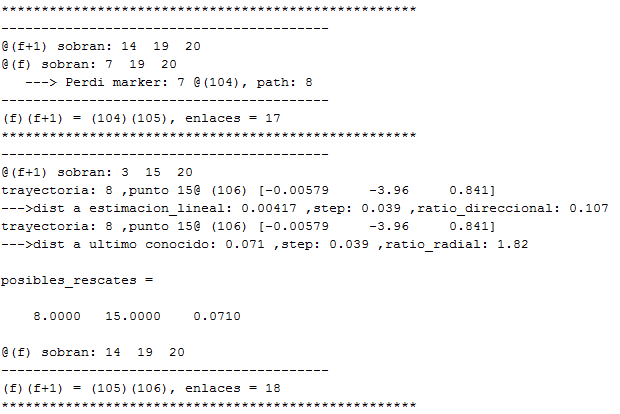
\includegraphics[scale=0.7]{img/Tracking/035_Salida_Codigo_Recuperacion.png}}\hspace{3 mm}
	
  \subfloat[Trayectoria]{
   \label{track_m8_recover}
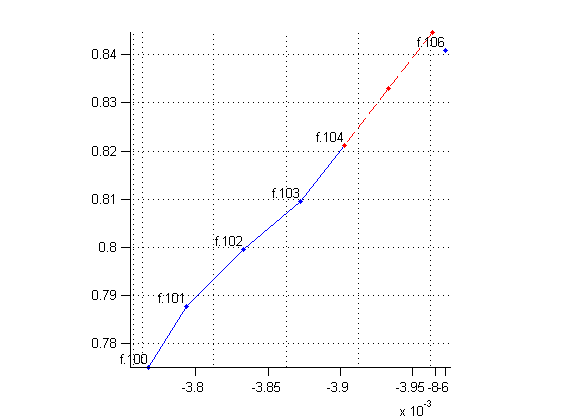
\includegraphics[scale=0.7]{img/Tracking/030_Inventario_trayectoria_direccional.png}}
\caption{Trayectoria perdida en frame 104, con posible candidato de recuperación en frame 106 por cercanía con la estimación por desplazamiento}
% Figura tomada de la reconstruccion 8_07_100_200
\label{inventario_trayectoria_direccional}
\end{figure} 
  
  \item \textbf{Distancia radial con respecto al ultimo punto conocido}. En algunos casos, la perdida del enlazado puede suceder cuando la trayectoria está en reposo (por ejemplo, un pie apoyado antes de volver a despegarse del suelo), o en transición (en el medio de una curva), por lo cual la estimación lineal anterior es invalida. Para ello, es útil relevar la distancia entre el ultimo punto conocido de una trayectoria trunca, y los puntos que no se enlazaron en [f+1]. Esta distancia, en caso de una posible recuperación, deberá ser proporcional al ultimo traslado conocido, por la diferencia temporal de frames entre el ultimo punto, y el posible candidato.
 
El procedimiento de validación indica que marcadores son inválidos, tanto usando el umbral global, como el individual, pero esta validación puede truncar una trayectoria durante el enlazado que luego debe ser estimada en caso de recuperación, o debe ser filtrado para el caso de post-procesamiento. Se debe establecer un procedimiento para tratar de recuperar estos marcadores, tratando de cumplir con las restricciones impuestas.
 
  
\end{enumerate} 

\end{itemize}

\subsubsection{Estimación de Marcadores Perdidos Durante Enlazado}

Si se encuentra algún punto que cumpla alguna de las condiciones de recuperación de trayectorias, es considerado para continuar la trayectoria, y deben estimarse los puntos intermedios para completar la trayectoria.

Esta estimación es realizada mediante mínimos cuadrados, donde las condiciones iniciales dependen de cuantos puntos de la trayectoria se tenían hasta el momento, la condición final es el punto encontrado en [f+1], las incógnitas son los puntos intermedios que se quieren encontrar, y las múltiples ecuaciones a cumplir son las planteadas en (\ref{track_var_acc}) y (\ref{track_acc}).

Sea $X_{[f+1]}$ un punto candidato por las condiciones anteriores, y el ultimo punto conocido en [f-1] de un trayectoria que pretende continuar, verifica [f-1]$\geq$3, entonces las ecuaciones que el punto a estimar $\boldsymbol{\tilde{X}_{[f]}}$ deberá cumplir, (observar que las ecuaciones de variación de aceleración son combinación lineal de las ecuaciones de aceleración)

\begin{equation}
\left\{
\begin{matrix}
X_{[f-3]} &-3.X_{[f-2]} &+3.X_{[f-1]} &-\boldsymbol{\tilde{X}_{[f]}} & &=0 \\
 &X_{[f-2]} &-3.X_{[f-1]} &+3.\boldsymbol{\boldsymbol{\tilde{X}_{[f]}}} &-X_{[f+1]} &=0 \\
 &X_{[f-2]} &-2.X_{[f-1]} &+\boldsymbol{\boldsymbol{\tilde{X}_{[f]}}} & &=0 \\
 & &X_{[f-1]} &-2.\boldsymbol{\boldsymbol{\tilde{X}_{[f]}}} &+X_{[f+1]} &=0 \\
\end{matrix}
\right.
\label{ecuaciones_estimacion_01}
\end{equation}

, escribiendo de forma matricial, separando los datos en incógnitas y condiciones,

\begin{equation}
\begin{split}
&\begin{pmatrix}
1 &-3 &3 &-1&0\\
0 &1 &-3 &3 &-1\\
0 &1 &-2 &1 &0\\
0 &0 &1 &-2 &1\\
\end{pmatrix}
\begin{pmatrix}
X_{[f-3]}\\
X_{[f-2]}\\
X_{[f-1]}\\
\boldsymbol{\tilde{X}_{[f]}}\\
X_{[f+1]}\\
\end{pmatrix} =
\begin{pmatrix}
1 &-3 &3\\
0 &1 &-3\\
0 &1 &-2\\
0 &0 &1\\
\end{pmatrix}
\begin{pmatrix}
X_{[f-3]}\\
X_{[f-2]}\\
X_{[f-1]}\\
\end{pmatrix}+
\begin{pmatrix}
-1\\
3\\
1\\
-2\\
\end{pmatrix}
\boldsymbol{\tilde{X}_{[f]}}+
\begin{pmatrix}
0\\
-1\\
0\\
1\\
\end{pmatrix}
X_{[f+1]} = 
\begin{pmatrix}
0\\
0\\
0\\
0\\
\end{pmatrix} \\
&\Rightarrow
\underbrace{
\begin{pmatrix}
-1\\
3\\
1\\
-2\\
\end{pmatrix}
}_{A_{[f]}}\boldsymbol{\tilde{X}_{[f]}} = \underbrace{- \begin{pmatrix}
1 &-3 &3\\
0 &1 &-3\\
0 &1 &-2\\
0 &0 &1\\
\end{pmatrix}
\begin{pmatrix}
X_{[f-3]}\\
X_{[f-2]}\\
X_{[f-1]}\\
\end{pmatrix} - \begin{pmatrix}
0\\
-1\\
0\\
1\\
\end{pmatrix}
X_{[f+1]}}_{B_{[f]}} \\
&\Rightarrow \boldsymbol{\tilde{X}_{[f]}} = \left( A_{[f]}^{t}.A_{[f]}\right)^{-1}.A_{[f]}^{t}.B_{[f]}
\end{split}
\label{matrices_estimacion_01}
\end{equation}

El procedimiento presentado para aproximación de puntos es análogo para el caso de tener $n$ frames a estimar entre el ultimo momento $f_{i}$ de una trayectoria, y su posible continuación en $f_{j}$, con $n+1=f_{j}-f_{i}$. Si $f_{i} \geq 3$ , se plantearán $n+1$ ecuaciones para variación de aceleración, y $n+1$ ecuaciones para variación de velocidad (aceleración), las cuales se resuelven de la misma forma. 

\begin{equation}
\left\{
\begin{matrix}
X_{[f_{i}-2]} &-3.X_{[f_{i}-1]} &+3.X_{[f_{i}]} &-\boldsymbol{\tilde{X}_{[f_{i}+1]}} & & & &=0 \\
& X_{[f_{i}-1]} &-3.X_{[f_{i}]} &+3.\boldsymbol{\tilde{X}_{[f_{i}+1]}} &-\boldsymbol{\tilde{X}_{[f_{i}+2]}} & & &=0 \\
& & X_{[f_{i}]} &-3.\boldsymbol{\tilde{X}_{[f_{i}+1]}} &+3.\boldsymbol{\tilde{X}_{[f_{i}+2]}} &-\boldsymbol{\tilde{X}_{[f_{i}+3]}}& &=0 \\
& & & \ddots & \ddots & \ddots & \ddots & \\
& & & \boldsymbol{\tilde{X}_{[f_{j}-3]}} &-3.\boldsymbol{\tilde{X}_{[f_{i}-j]}} &+3.\boldsymbol{\tilde{X}_{[f_{j}-1]}} &-X_{[f_{j}]} &=0 \\
\end{matrix}
\right.
\label{ecuaciones_estimacion_n}
\end{equation}

En caso que la información previa a la perdida es menor, con $f_{i} \geq 2$, se plantea una ecuación menos, aquella que plantea la variación de aceleración de aceleración con el primer elemento incógnita que es la única que precisaría tres elementos previos, las otras ecuaciones no tienen problemas para plantearse.

Esta metodología de estimación de puntos intermedios es retomada para la validación en trayectoria, donde las incógnitas pasan a ser lo puntos que deben ser regularizados debido a presentar aceleración excesiva y discontinua para el marcador ( como fue establecido al principio de esta sección).




\subsection{Resultados y Análisis}

El objetivo del bloque de seguimiento es identificar los puntos reconstruidos, presentarlos como trayectorias, y corregirlos si es necesario. Por esta razón, es esperable que para una misma secuencia, los resultados sean similares a la reconstrucción, siendo las únicas leves diferencias las correcciones realizadas sobre trayectorias particulares, y la posibilidad de medir el error por marcador individual ya que a esta altura del algoritmo ya están identificados las distintas trayectorias. Los siguientes resultados fueron probados sobre una captura sintética de 113 frames, 14 marcadores, a lo largo de 17 cámaras.

\begin{figure}[hbt]
\begin{center}
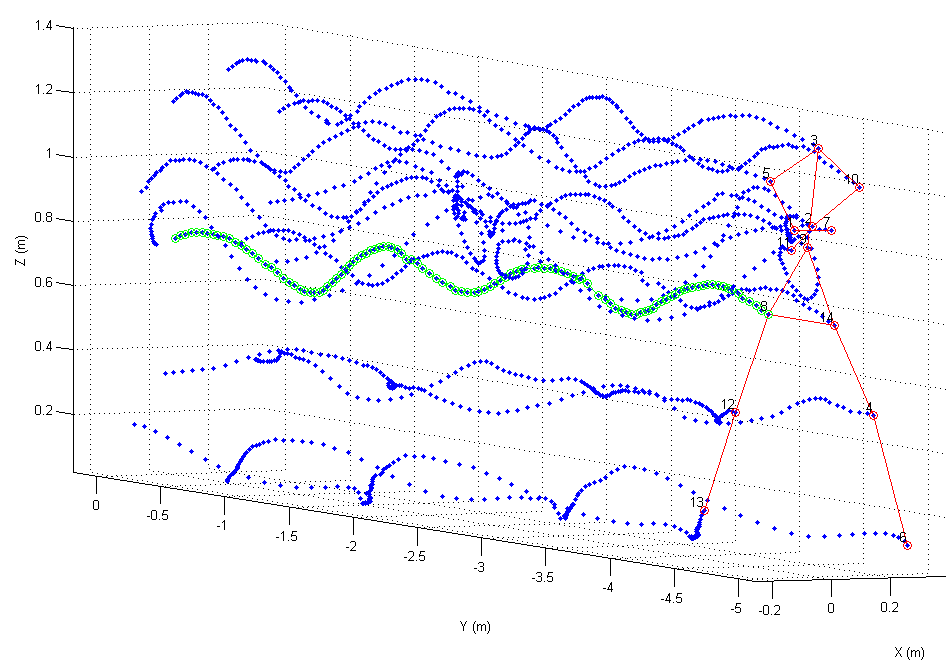
\includegraphics[width=\linewidth]{img/Tracking/040_Salida_Tracking_Esqueleto_Trayectoria.png}
\end{center}
\caption{Tracking sobre captura sintética, 113 frames, 17 cámaras, 14 marcadores}
\label{Tracking_Esqueleto_Trayectoria}
\end{figure}

El filtrado y validación por trayectorias, permite reducir el error máximo y mejorar el promedio de trayectorias especificas (marcador 8 en figura), pero al aplicar global mente puede perjudicar a aquellas trayectorias que tengan naturalmente discontinuidades en aceleración debido a variaciones abruptas de movimiento (Tabla \ref{tablaerrortrack}). Para todos los marcadores, el error promedio se encuentra por debajo de 0.5 cm para la reconstrucción sobre vídeos sintéticos de la secuencia CMU-8-07-100-200 con 17 cámaras, y con el filtrado por aceleración individual de marcadores. En otras capturas, los comportamientos son similares con promedios inferiores a 0.5 cm, y errores máximos por debajo de 3 cm, para el caso de reconstrucción con 17 cámaras.Mas adelante se estudiará el impacto de cambiar los conjunto de cámaras en marcadores   

\begin{table}[h]
\begin{tabular}{|c|c|c|c|c|c|c|}
\hline
\begin{tabular}[c]{@{}c@{}}Marker\\ Track\end{tabular} & \begin{tabular}[c]{@{}c@{}}Marker\\ Ground\end{tabular} & \begin{tabular}[c]{@{}c@{}}Name\\ Ground\end{tabular}       & \begin{tabular}[c]{@{}c@{}}Error\\ Promedio(cm)\end{tabular} & \begin{tabular}[c]{@{}c@{}}Percentil\\ 99\%(cm)\end{tabular} & \begin{tabular}[c]{@{}c@{}}Error Promedio\\ (filtrado)(cm)\end{tabular} & \begin{tabular}[c]{@{}c@{}}Percentil 99\%\\ (filtrado)(cm)\end{tabular} \\ \hline
12       & 1         & LeftUpLeg          & 0,3671                                                       & 0,5158                                                       & 0,4042                                                                  & 2,0371                                                                  \\ \hline
3        & 2         & LeftLeg            & 0,367                                                        & 0,5411                                                       & 0,5456                                                                  & 2,7576                                                                  \\ \hline
2        & 3         & LeftFoot           & 0,372                                                        & 0,558                                                        & 0,377                                                                   & 0,7558                                                                  \\ \hline
6        & 4         & RightUpLeg         & 0,3714                                                       & 0,5879                                                       & 0,4033                                                                  & 1,6849                                                                  \\ \hline
4        & 5         & RightLeg           & 0,378                                                        & 0,586                                                        & 0,446                                                                   & 2,1396                                                                  \\ \hline
14       & 6         & RightFoot          & 0,4212                                                       & 1,8483                                                       & 0,4447                                                                  & 1,8483                                                                  \\ \hline
9        & 7         & Spine              & 0,404                                                        & 0,6043                                                       & 0,4103                                                                  & 0,7652                                                                  \\ \hline
7        & 8         & Head               & 0,3867                                                       & 0,9063                                                       & 0,3923                                                                  & 1,2422                                                                  \\ \hline
8        & 9         & LeftArm            & 0,3666                                                       & 0,7997                                                       & 0,3617                                                                  & 0,594                                                                   \\ \hline
13       & 10        & LeftForeArm        & 0,3873                                                       & 0,9056                                                       & 0,3961                                                                  & 1,1897                                                                  \\ \hline
10       & 11        & LeftHand           & 0,4007                                                       & 1,1722                                                       & 0,4128                                                                  & 1,4842                                                                  \\ \hline
1        & 12        & RightArm           & 0,4025                                                       & 1,4771                                                       & 0,3866                                                                  & 0,944                                                                   \\ \hline
11       & 13        & RightForeArm       & 0,3844                                                       & 0,781                                                        & 0,3945                                                                  & 0,8591                                                                  \\ \hline
5        & 14        & RightHand          & 0,3816                                                       & 0,7728                                                       & 0,411                                                                   & 1,1087                                                                  \\ \hline
         &           & \textbf{Secuencia} & \textbf{0,35686}                                             & \textbf{0,81266}                                             & \textbf{0,38305}                                                        & \textbf{1,6747}                                                         \\ \hline
\end{tabular}
\caption{Medida de error de tracking en captura de la base de datos sintética.}
\label{tablaerrortrack}
\end{table}

\begin{figure}[H]
 \centering
  \subfloat[Trayectoria sin Corregir Por Aceleración]{
	\label{Salida_Tracking_Original}
	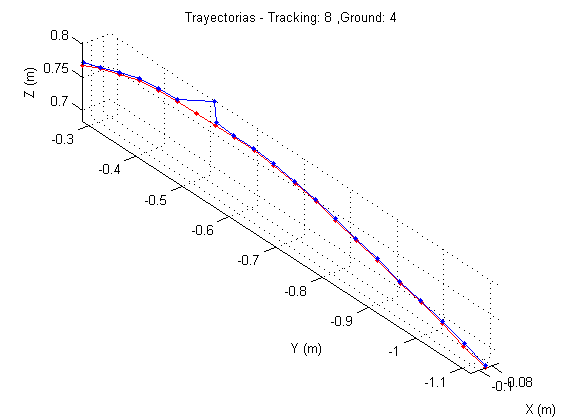
\includegraphics[scale=0.5]{img/Tracking/036_Salida_Tracking_Original.png}}
  \subfloat[Trayectoria Corregida Por Aceleración]{
   \label{Salida_Tracking_Filtrado}
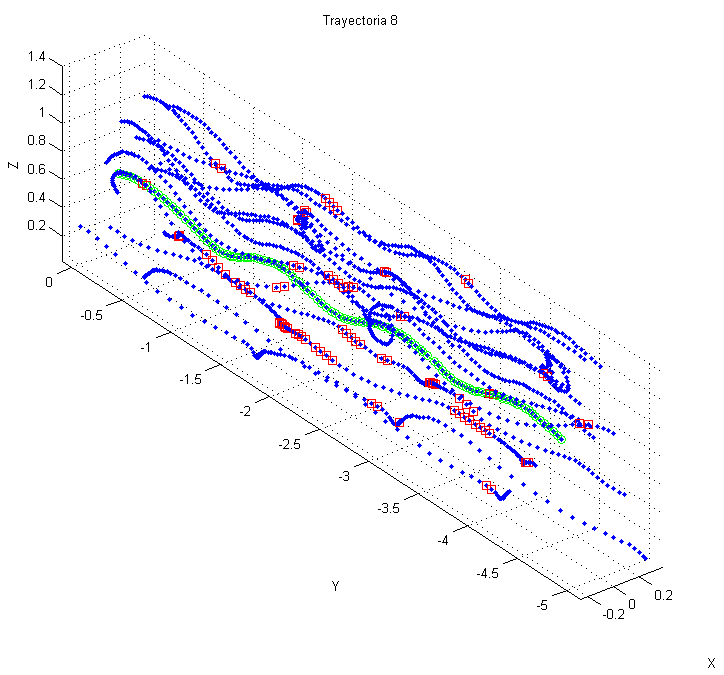
\includegraphics[scale=0.5]{img/Tracking/037_Salida_Tracking_Filtrado.png}}
\hspace{3 mm}
  \subfloat[Error de Marcador, sin Corregir]{
	\label{Salida_Tracking_Original}
	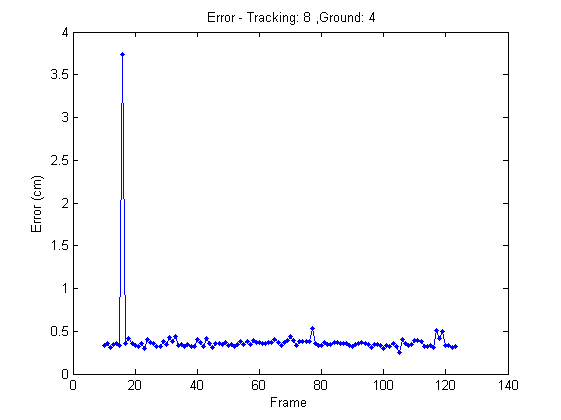
\includegraphics[scale=0.5]{img/Tracking/038_Salida_Tracking_Error_Marker_8_original.png}}
  \subfloat[Error de Marcador, Corregido]{
   \label{Salida_Tracking_Filtrado}
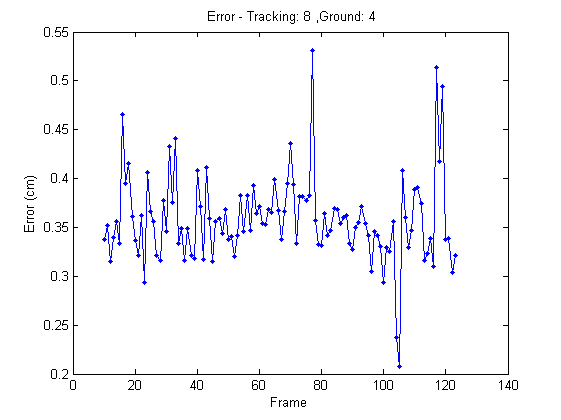
\includegraphics[scale=0.5]{img/Tracking/039_Salida_Tracking_Error_Marker_8_filtrado.png}}
\caption{Corrección por variación de aceleración, medidas de error antes y después de corregir}
% Figura tomada de la reconstruccion 8_07_100_200
\label{Tracking_Original_Filtrado_Errores}
\end{figure}


Al tener las etiquetas constantes para las trayectorias, es posible visualizar la relación entre marcadores, quedando pendientes medidas adicionales para robustecer el sistema, como imponer restricciones al movimiento entre marcadores en un mismo miembro, por imponer no solo continuidad en aceleración de marcadores sino ángulos de articulaciones y huesos. Esta continuidad debe tener cierta tolerancia debido a que los marcadores son representativos de articulaciones, y no se mueven completamente solidarios por lo que existen leves variaciones en las distancias entre marcadores, como se observa en la figura \ref{distancia_angulo_marcadores_piernas}, correspondiente a los marcadores asociados a la pierna en la captura 8\_03\_100\_100. En este caso se observa la continuidad y periodicidad de el angulo entre marcadores así como la constancia de la distancia, salvo momentos ocasionales, asociados a momentos específicos de la captura (cuando el pie rompe el reposo por ejemplo, antes de dar otro paso) ,sin ser mayor a los pocos centímetros en momentos puntuales y recuperables en régimen.

\begin{figure}[H]
 \centering
  \subfloat[Trayectorias de marcadores de pierna]{\includegraphics[scale=0.45]{img/Tracking/050_Salida_Tracking_13_14_10.png} %\label{trayectorias_marcadores_piernas}
   }	
  \subfloat[Distancia y Angulo entre marcadores de la pierna]{\includegraphics[scale=0.45]{img/Tracking/051_Salida_Angulo_Distancia_13_14_10.png}\label{distancia_angulo_marcadores_piernas}}
\caption{Ejemplos de Posibles restricciones en angulo y distancia, para el caso de la pierna en marcha}
\label{restricciones_tracking}
\end{figure}


\section{Discusión y análisis de resultados}


\section{Conclusiones}
%conclusiones, pendientes, etc

En esta sección se evaluarán las conclusiones obtenidas a partir de lo realizado en el proyecto. Las mismas se pueden separar en conclusiones generales, y en particulares de los capítulos vistos anteriormente.

Como conclusiones generales se presentan las siguientes:
\begin{itemize}
\item Se cumplió el objetivo principal: se logró obtener un sistema completo que a partir de las capturas de video de una persona en un ambiente de laboratorio con las condiciones adecuadas, obtiene la posición 3D de  los marcadores presentes en el cuerpo de dicha persona, logrando representar su movimiento con una presición del orden del centímetro.
\item Se logró relevar la literatura existente, y se realizó una clasificación de los documentos de acuerdo a la relevancia que prestan para construir un sistema de estas características. 
\item Se relevó el software existente, y se buscaron implementaciones en matlab, C/C++ y otros lenguajes, pero no se encontró un software Open Source que se adaptara a las características necesarias para utilizar de base en este proyecto. Debido a esto, se decidió implementar los bloques por cuenta propia, utilizando algunos algoritmos básicos de procesamiento de imagenes ya implementados o realizados especificamente para este proyecto. Esta etapa por momentos tuvo un carácter más de investigación científica que de proyecto ingenieril.
\item Se identificaron los distintos casos de uso, y se decidió implementar el sistema en base al caso de uso de marcha.
\item Se lograron implementar los 4 grupos de algoritmos principales que componen la aplicación: calibración, detección de marcadores, estimación de pose (o reconstrucción) y seguimiento.
\item Se generó un sistema que integra los 4 bloques nombrados en el punto anterior, y que dada la entrada definida obtiene la salida esperada.
\item Se elaboró una interfaz gráfica de usuario (GUI) básica para que el sistema pueda ser utilizado de una forma más práctica y amigable por el usuario.
\item Se buscaron bases de datos que se encuentren dentro de las hipótesis del problema, de forma tal de probar el mismo para diferentes casos y evaluar su rendiemiento. Debido a que no se encontró ninguna base de datos disponible que cumpla con las características deseadas, se elaboró una en base a secuencias sintéticas generadas en Blender.
\item Se generó un conjunto de benchmarks\footnote{Herramientas de evaluación de performance.}, capaces de obtener una buena medida del rendimiento del sistema. 
\end{itemize}

A continuación, se plantean las conclusiones específicas de las etapas principales del proyecto:
\begin{itemize}
	\item Relevamiento bibliográfico
	\begin{itemize}
		\item No se encontraron implementaciones de sistemas de captura de movimiento Open Source con las características del sistema de este proyecto. 
	\end{itemize}
	\item Base de datos
	\item Calibración
	\item Detección de marcadores
	\begin{itemize}
		\item Se logró implementar un conjunto de algoritmos capaces de detectar la posición 2D de los marcadores en el cuerpo del paciente para todo instante de tiempo y exponer los resultados en un archivo XML. 
		\item Los resultados correspondientes a las pruebas con secuencias cintéticas fueron muy buenos, logrando un error que en la mayoría de los casos se ubicó por debajo de los 4 píxeles.
		\item Por el lado del procesamiento de secuencias reales, no se consiguieron secuencias que estén exactamente en las hipótesis del probelma. Aún asi, se realizaron pruebas con secuencias que se asemejaban a las condiciones necesarias obteniendo buenos resultados al extraer el fondo de la captura.
		\item Se observó que para ambientes donde las condiciones se mantienen constantes a lo largo del tiempo (como por ejemplo en un laboratorio), el umbral no cambia significativamente su valor, pudiendose utilzar un valor constante en el para toda una secuencia. Esto permite ahorrar tiempo de procesamiento y reduce el costo computacional de la detección.
		\item Se observó que se puede mejorar la detección, ajustando los valores de las constantes $A$ y $B$ del filtro circular (ver seccióm \ref{implementSegment}) de forma tal de hacer el filtro más selectivo o menos.
	\end{itemize}
	\item Reconstrucción
	\item Segumiento
	\item Medida de performance
	\begin{itemize}
		\item Se obtuvo una precisión en la detección de los marcadores, del orden del centímetro.
		\item El máximo error no superó los 5 cm.
		\item Se obtuvieron muy buenos resultados, logrando reconstruir todos los marcadores en toda la secuencia hasta con un mínimo de 6 cámaras. Con menos cámaras se pierden marcadores ocasionalmente.
		\item Para el caso de 6 cámaras, la correcta detección del movimiento depende de la posición que tengan estas en el espacio.
	\end{itemize}
\end{itemize}

Cabe destacar que por temas de cronograma y de presupuesto, en muchos aspectos no se utilizó la tecnología más moderna (por ejemplo sensores infrarrojos, cámaras de mejor calidad, etc.) que de haberlas utilizado se hubiesen logrado mejores resultados. Si bien esta primera versión del sistema no está a la altura de los sistemas comerciales vistos en este documento, se logró dar el primer paso y se dejaron todas las condiciones necesarias para poder continuar con el proyecto y llevar el mismo al nivel de las otras herramientas.

Quedan como tareas pendientes para etapas futuras:
\begin{itemize}
	\item Probar el sistema en un laboratorio con las características definidas en este proyecto y con más de 6 cámaras previamente calibradas.
	\item Adaptar el sistema para otros casos de uso además de la marcha.
	\item Robustecer la segmentación, ya sea agregando algoritmos que complementen la umbralización de Otsu\cite{otsu} o cambiando la umbralización por un algoritmo más complejo.
	\item Mejorar la interfáz gráfica de usuario, haciéndola más amigable e intuitiva, de forma tal que el especialista pueda utilizarla como una aplicación de usuario.
	\item Realizar un manual de usuario.
\end{itemize}

\begin{thebibliography}{1}
\label{Referencias}

\bibitem{herda} Herda L., Fua P., Plankers R., Boulic R. Using skeleton-based tracking to increase the reliability of optical motion capture.Human movement science, 20(3), 313-341, 2001.
\bibitem{griegos} Malik N., Dracos T. \& Papantoniou D. (1993). Particle tracking in three-dimensional turbulent flows - Part II: Particle tracking, Experiments in Fluids, 15:279–294.
\bibitem{faugueras} Faugeras o., Robert L. What can two images tell us about a third one. International Journal of Computer vision, 18(1), 485-492,1996.
\bibitem{colombianos} C.A.Diaz, M.L.Toro, J.C.Forero, A.Torres Detección, rastreo y reconstrucción tridimensional de marcadores pasivos para análisis de movimiento humano. Cinemed iii
Revista ingeniería Biomédica issn 1909-9762, volumen 3, número 6, julio-diciembre 2009, págs. 56-67 Escuela de Ingeniería de Antioquia-Universidad ces, Medellín, Colombia
\bibitem{surveyThreshold} M.Sezgin,B.Sankur, “Survey over image thresholding techniques and quantitative performance evaluation”, Journal of Electronic Imaging 13(1), 146–165 (January 2004).
\bibitem{histImgRef} http://deploy.virtual$\-$labs.ac.in/labs/cse19/theory.php?exp=segment
\bibitem{Gonzalez} Digital Image Processing. Rafael Gonzalez  \& Richard Woods.
\bibitem{smooth} pág. 174, sección 3.5 Digital Image Processing. Rafael Gonzalez  \& Richard Woods.
\bibitem{tophat} pág. 692, sección 9.6.3 Digital Image Processing. Rafael Gonzalez  \& Richard Woods.
\bibitem{segment} pág. 760, sección 10.3 Digital Image Processing. Rafael Gonzalez  \& Richard Woods.
\bibitem{otsu} Nobuyuki Otsu (1979). "A threshold selection method from gray-level histograms". IEEE Trans. Sys., Man., Cyber.
\bibitem{implementacionOtsu} Matías Tailanian, Juan Cardelino. https://github.com/martin-etchart/kde 24/11/2014.
\bibitem{bayes} pág. 894, sección 12.2.2 Digital Image Processing. Rafael Gonzalez  \& Richard Woods.
\bibitem{procImg} D. Phillips; “Image Processing in C: Analyzing and Enhancing Digital Images”, RandD Publications, 1994
\bibitem{opencv} http://opencv.org/
\bibitem{cvblob} https://code.google.com/p/cvblob/
\bibitem{betweenvarianze} sección 4.4.4, http://homepages.inf.ed.ac.uk/rbf/CVonline/LOCAL{\_}COPIES/MORSE/threshold.pdf
\bibitem{kinect} http://www.xbox.com/es-ES/Kinect
\bibitem{xml} http://es.wikipedia.org/wiki/Extensible{\_}Markup{\_}Language
\bibitem{HSV} Shamik Sural, Gang Qian and Sakti Pramanik (2002). "Segmentation And Histogram Generation Using The HSV Color Space For Image Retrieval". Michigan State University, USA.
\bibitem{defBlob} http://en.wikipedia.org/wiki/Binary{\_}large{\_}object

\end{thebibliography}

\end{document}